%\title{Honors Thesis Presentation}
\documentclass[10pt]{beamer}

\usetheme[progressbar=frametitle]{metropolis}
\usepackage{appendixnumberbeamer}

\usepackage[compatibility=false]{caption}
\usepackage{subcaption}
\usepackage{csquotes}
\usepackage{booktabs}
\usepackage{hyperref}
\usepackage[scale=2]{ccicons}
\usepackage{tikz}
\usetikzlibrary{positioning}
\usetikzlibrary{3d}

\usepackage{multimedia}
\usepackage{media9}

\usepackage{pgfplots}
\usepgfplotslibrary{dateplot}

\usepackage{xspace}
\newcommand{\themename}{\textbf{\textsc{metropolis}}\xspace}

\title{Evolvability: What is It \newline and How Do We Get It?}
\subtitle{Coolidge Otis Chapman Honors Program}
\date{March 22nd, 2017}
\author{\texorpdfstring{Matthew Moreno \newline\url{mamoreno@pugetsound.edu}}{Matthew Moreno}}
\titlegraphic{\hfill
\includegraphics[height=2cm]{img/UofPS_stacked_maroonRGB_PNG.png}}

%cyan 36a8b8
%blue b2d4ef
%purple c677dd
%overleaf green 4F9C45
%green 7b9e62
%red 1 cb4752
%red 2 be5046
%orange 1 d19a66
%orange 2 e5c07b

\definecolor{h1}{HTML}{d19a66}
\definecolor{h2}{HTML}{36a8b8}

\begin{document}

\maketitle

% \begin{frame}{Table of contents}
%   \setbeamertemplate{section in toc}[sections numbered]
%   \tableofcontents[hideallsubsections]
% \end{frame}

\section{Evolutionary Algorithm}

\begin{frame}{Search}
  \begin{columns}
  \column{0.5\textwidth}
  \centering
   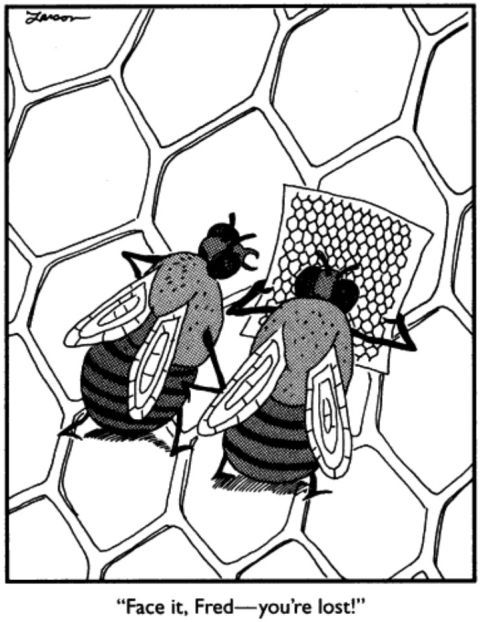
\includegraphics[height=\textwidth]{img/farside}
   \column{0.5\textwidth}
   \begin{itemize}
      \item \alert{common scenario:} you can recognize a good solution, but you don't know how to find one
      \item encountered by computer scientists (and everyone else, too)
      \item \alert{common approach:} try different options, evaluate outcomes to help choose next options to try
       \item this is called \alert{search}    
       \end{itemize}
   \end{columns}
\end{frame}

\begin{frame}{Evolutionary Algorithm}

\begin{columns}
\begin{column}{0.25\textwidth}
\begin{itemize}
  \item individual
  \item population
  \item fitness function
  \item selection
  \item mutation
  \item genotype
  \item phenotype
\end{itemize}
\end{column}
\begin{column}{0.75\textwidth}
\begin{figure}
  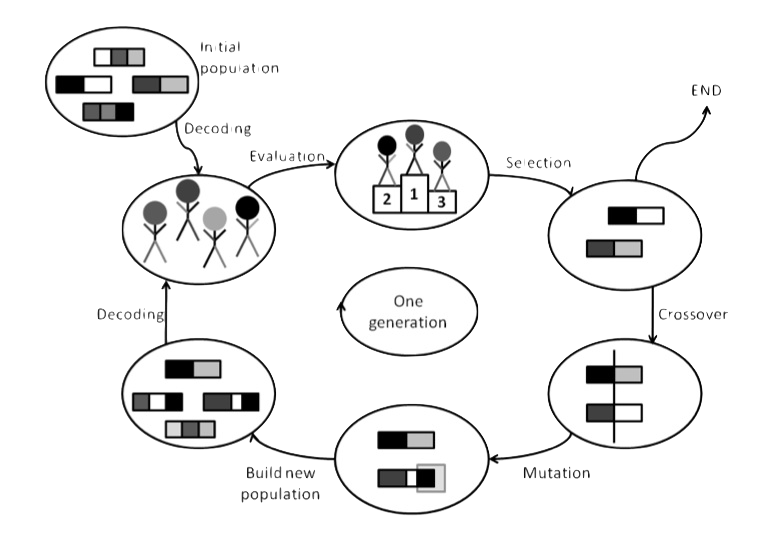
\includegraphics[width=\textwidth]{img/working_principle_of_EA.png}
  \captionsetup{singlelinecheck=off,justification=raggedright}
  \caption{A schematic illustration of the evolutionary algorithm \cite[Figure 1]{Prothmann2009EvolutionaryOptimisation}.}
\end{figure}
\end{column}
\end{columns}
    
\end{frame}


\begin{frame}{Evolutionary Algorithm}
\begin{figure}
  \includemedia[width=\linewidth,height=0.6\textwidth, flashvars={scaleMode=zoom}]{}{http://www.youtube.com/v/z9ptOeByLA4?t=1m08s&amp;rel=0&amp;showinfo=0}
  \captionsetup{singlelinecheck=off,justification=raggedright}
\href{https://youtu.be/z9ptOeByLA4?t=1m08s}{\caption{Evolution in Action \cite{Cheney2013UnshacklingEncoding}}}
\end{figure}
\end{frame}

\begin{frame}{Evolutionary Algorithm: Problem Statement}
  What makes an evolutionary algorithm work?
\end{frame}

\section{Defining Evolvability}

\begin{frame}{Defining Evolvability}
consensus: the amount of \textcolor{h2}{useful} \textcolor{h1}{variation} generated by the evolutionary process
\begin{itemize}
  \item evolvability as the amount of \textcolor{h1}{\textbf{novel variation}} generated
  \item evolvability the proportion of variation that is \textcolor{h2}{\textbf{useful}}
\end{itemize}
\end{frame}

% \begin{frame}{The Evolvability Conundrum}
% How can natural selection ``favor properties hat may prove useful to a given lineage in the future, but have no present adaptive function''? \cite{Pigliucci2008IsEvolvable}
% \end{frame}


\subsection{Evolvability as Novel Variation}

\begin{frame}{Evolvability as Novel Variation}
	\begin{figure}
 \centering
    \begin{subfigure}[b]{0.5\textwidth}
        \centering
    	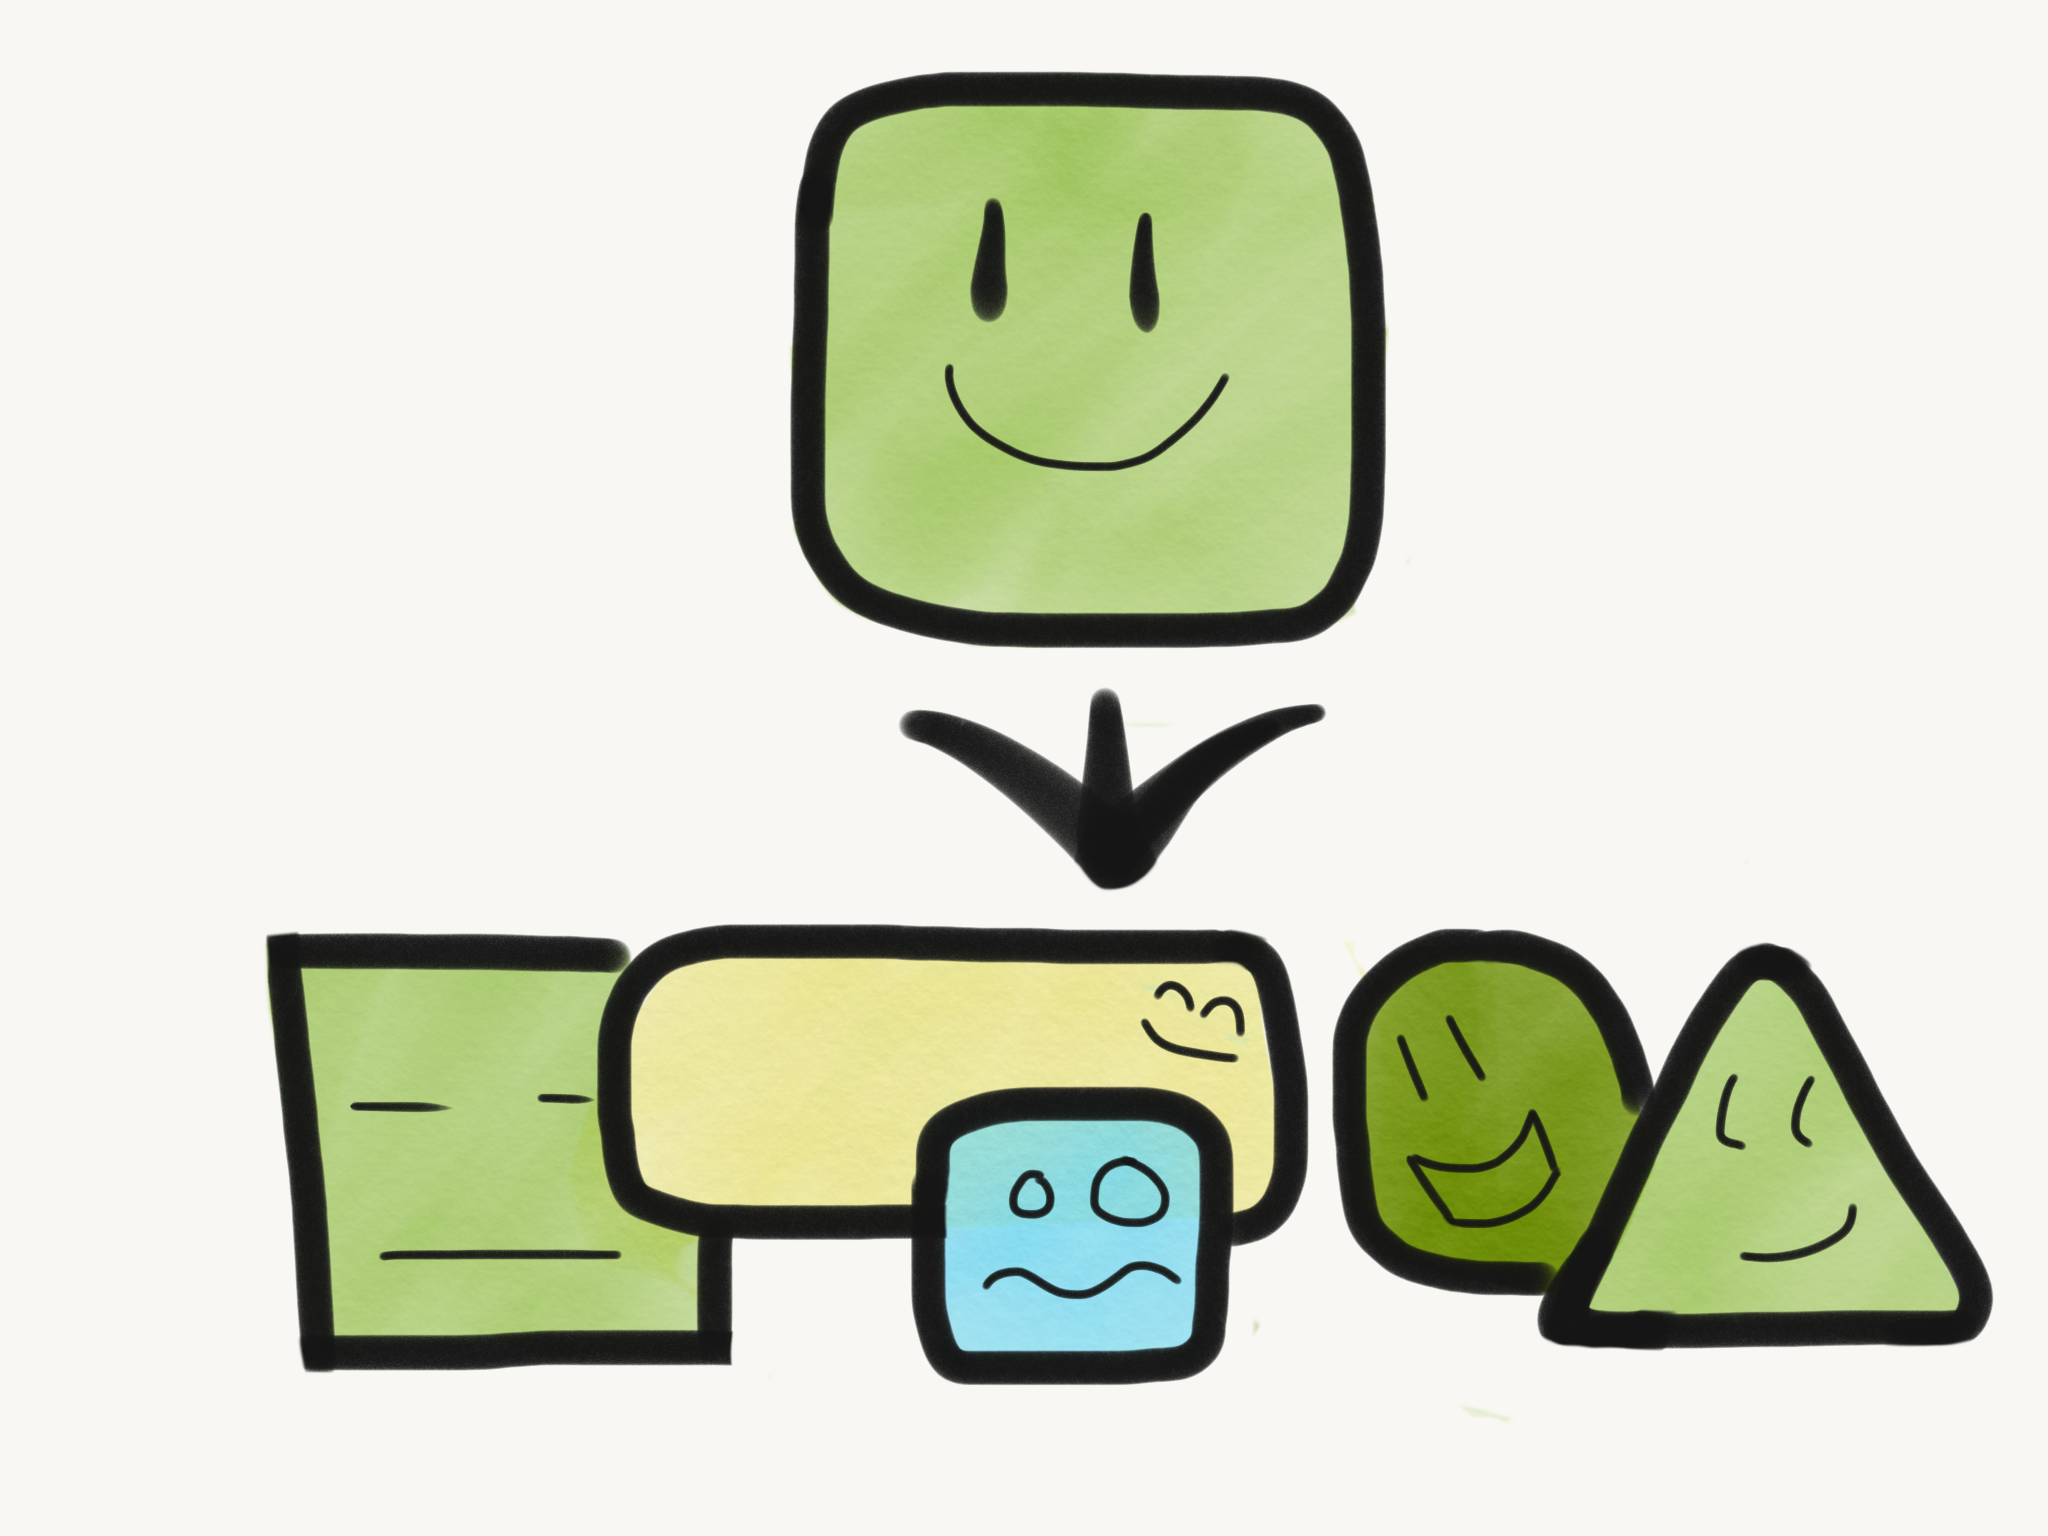
\includegraphics[width=\textwidth]{img/individual_evolvability.png}
        \caption{high individual evolvability}
        \label{subfig:canalization}
    \end{subfigure}%
    \hfill
    \begin{subfigure}[b]{0.5\textwidth}
        \centering
        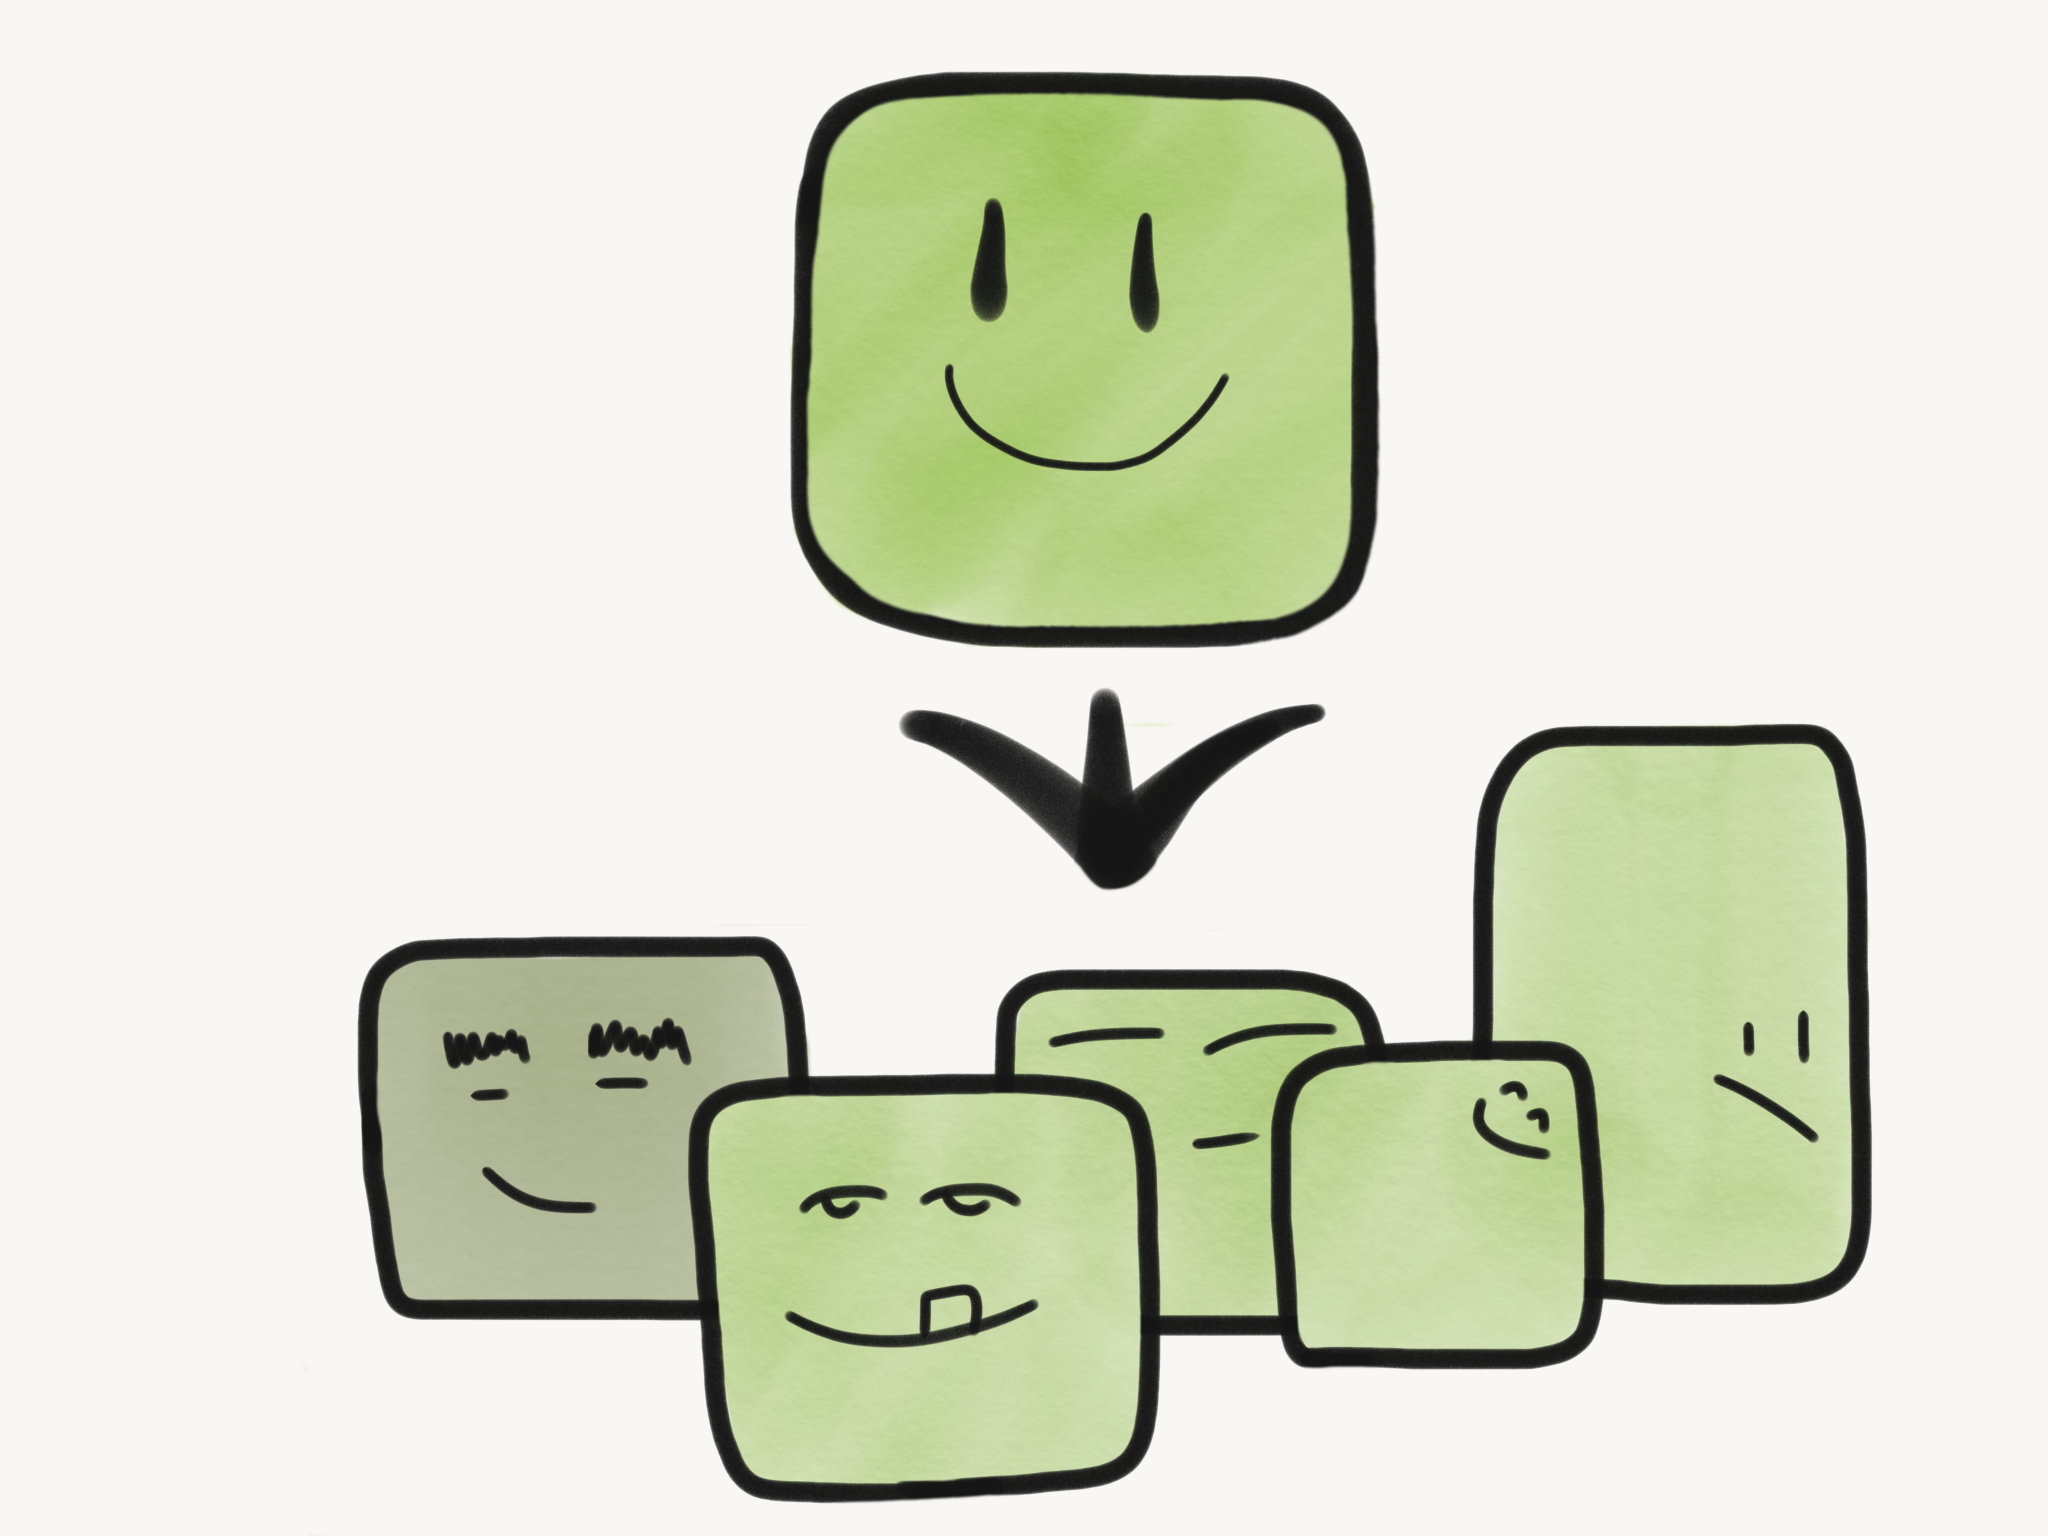
\includegraphics[width=\textwidth]{img/low_individual_evolvability.png}
        \caption{low individual evolvability}
        \label{subfig:no_canalization}
    \end{subfigure}
 	\captionsetup{singlelinecheck=off,justification=raggedright}
    \vspace{-4ex}
  \captionsetup{singlelinecheck=off,justification=raggedright}
  \caption{An illustration of individual evolvability, considering evolvability as heritable variation \cite{Wilder2015ReconcilingEvolvability}.}
  \label{fig:high_vs_low_individual_evolvability}
\end{figure}
\end{frame}

\subsection{Evolvability as Bias towards Useful Variation}

\begin{frame}{Evolvability as Bias towards Useful Variation}
  \begin{figure}
    \centering
    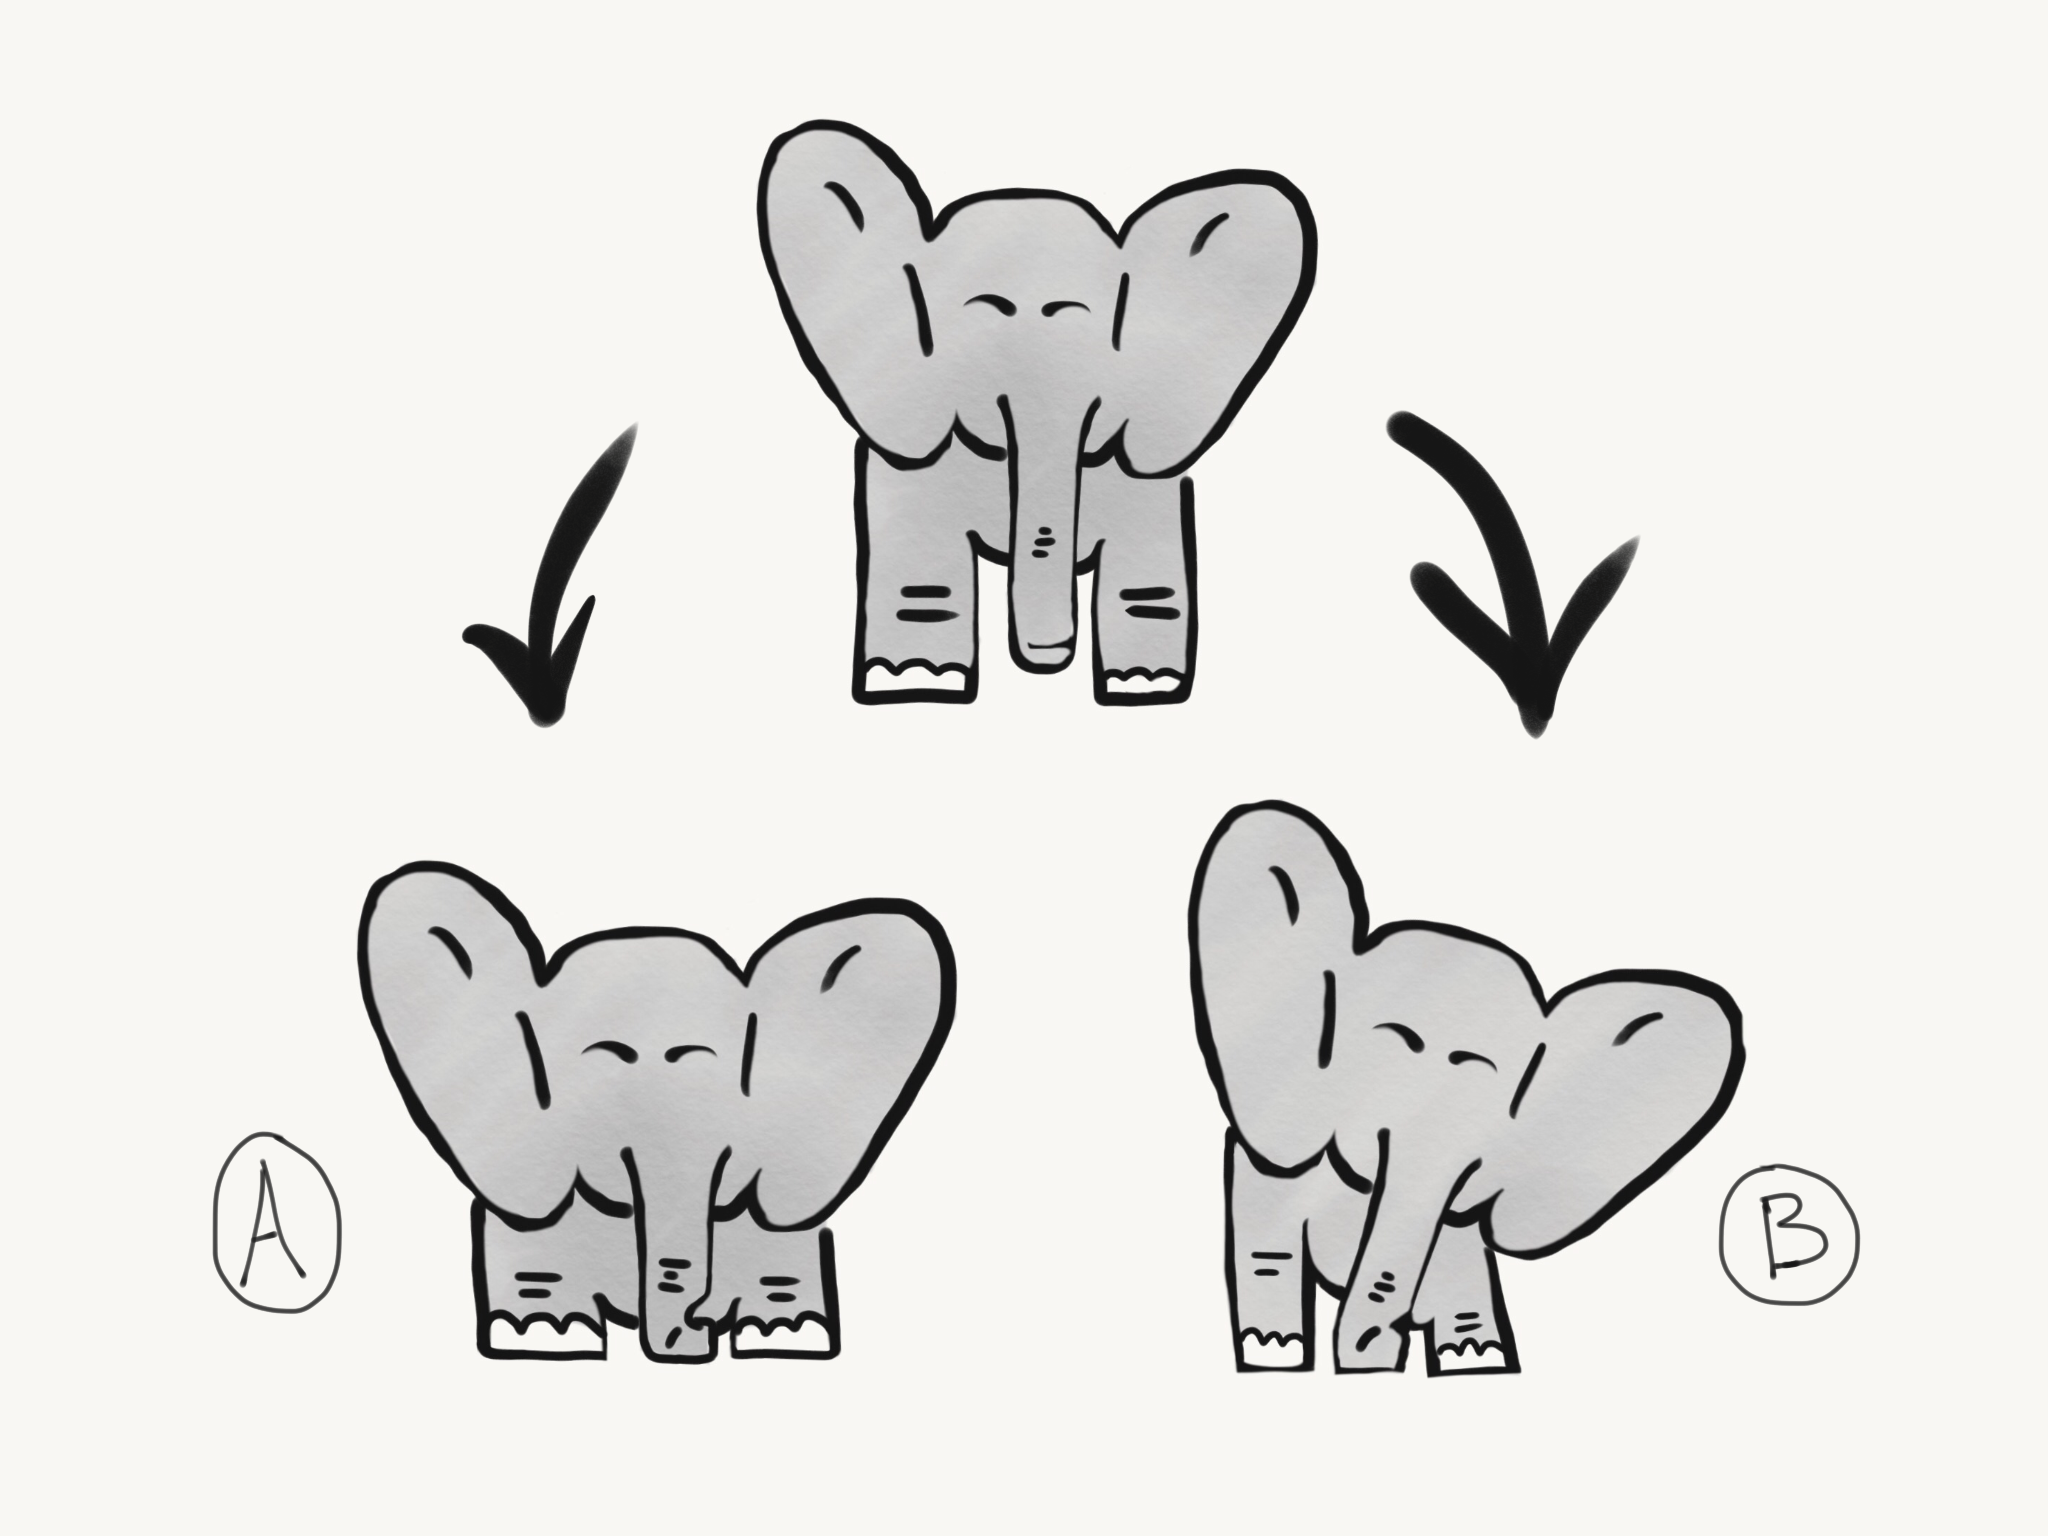
\includegraphics[width=0.8\textwidth]{img/developmental_constraint}
 	\captionsetup{singlelinecheck=off,justification=raggedright}
  	\caption{Illustration of developmental constraint; high evolvability left and low evolvability right \cite{Smith1985DevelopmentalBiology,Tuinstra1990LackDevelopment}.}
    \label{fig:developmental_constraint}
\end{figure}
\end{frame}

\begin{frame}{Evolvability as Bias towards Useful Variation}
  \begin{figure}
    \centering
    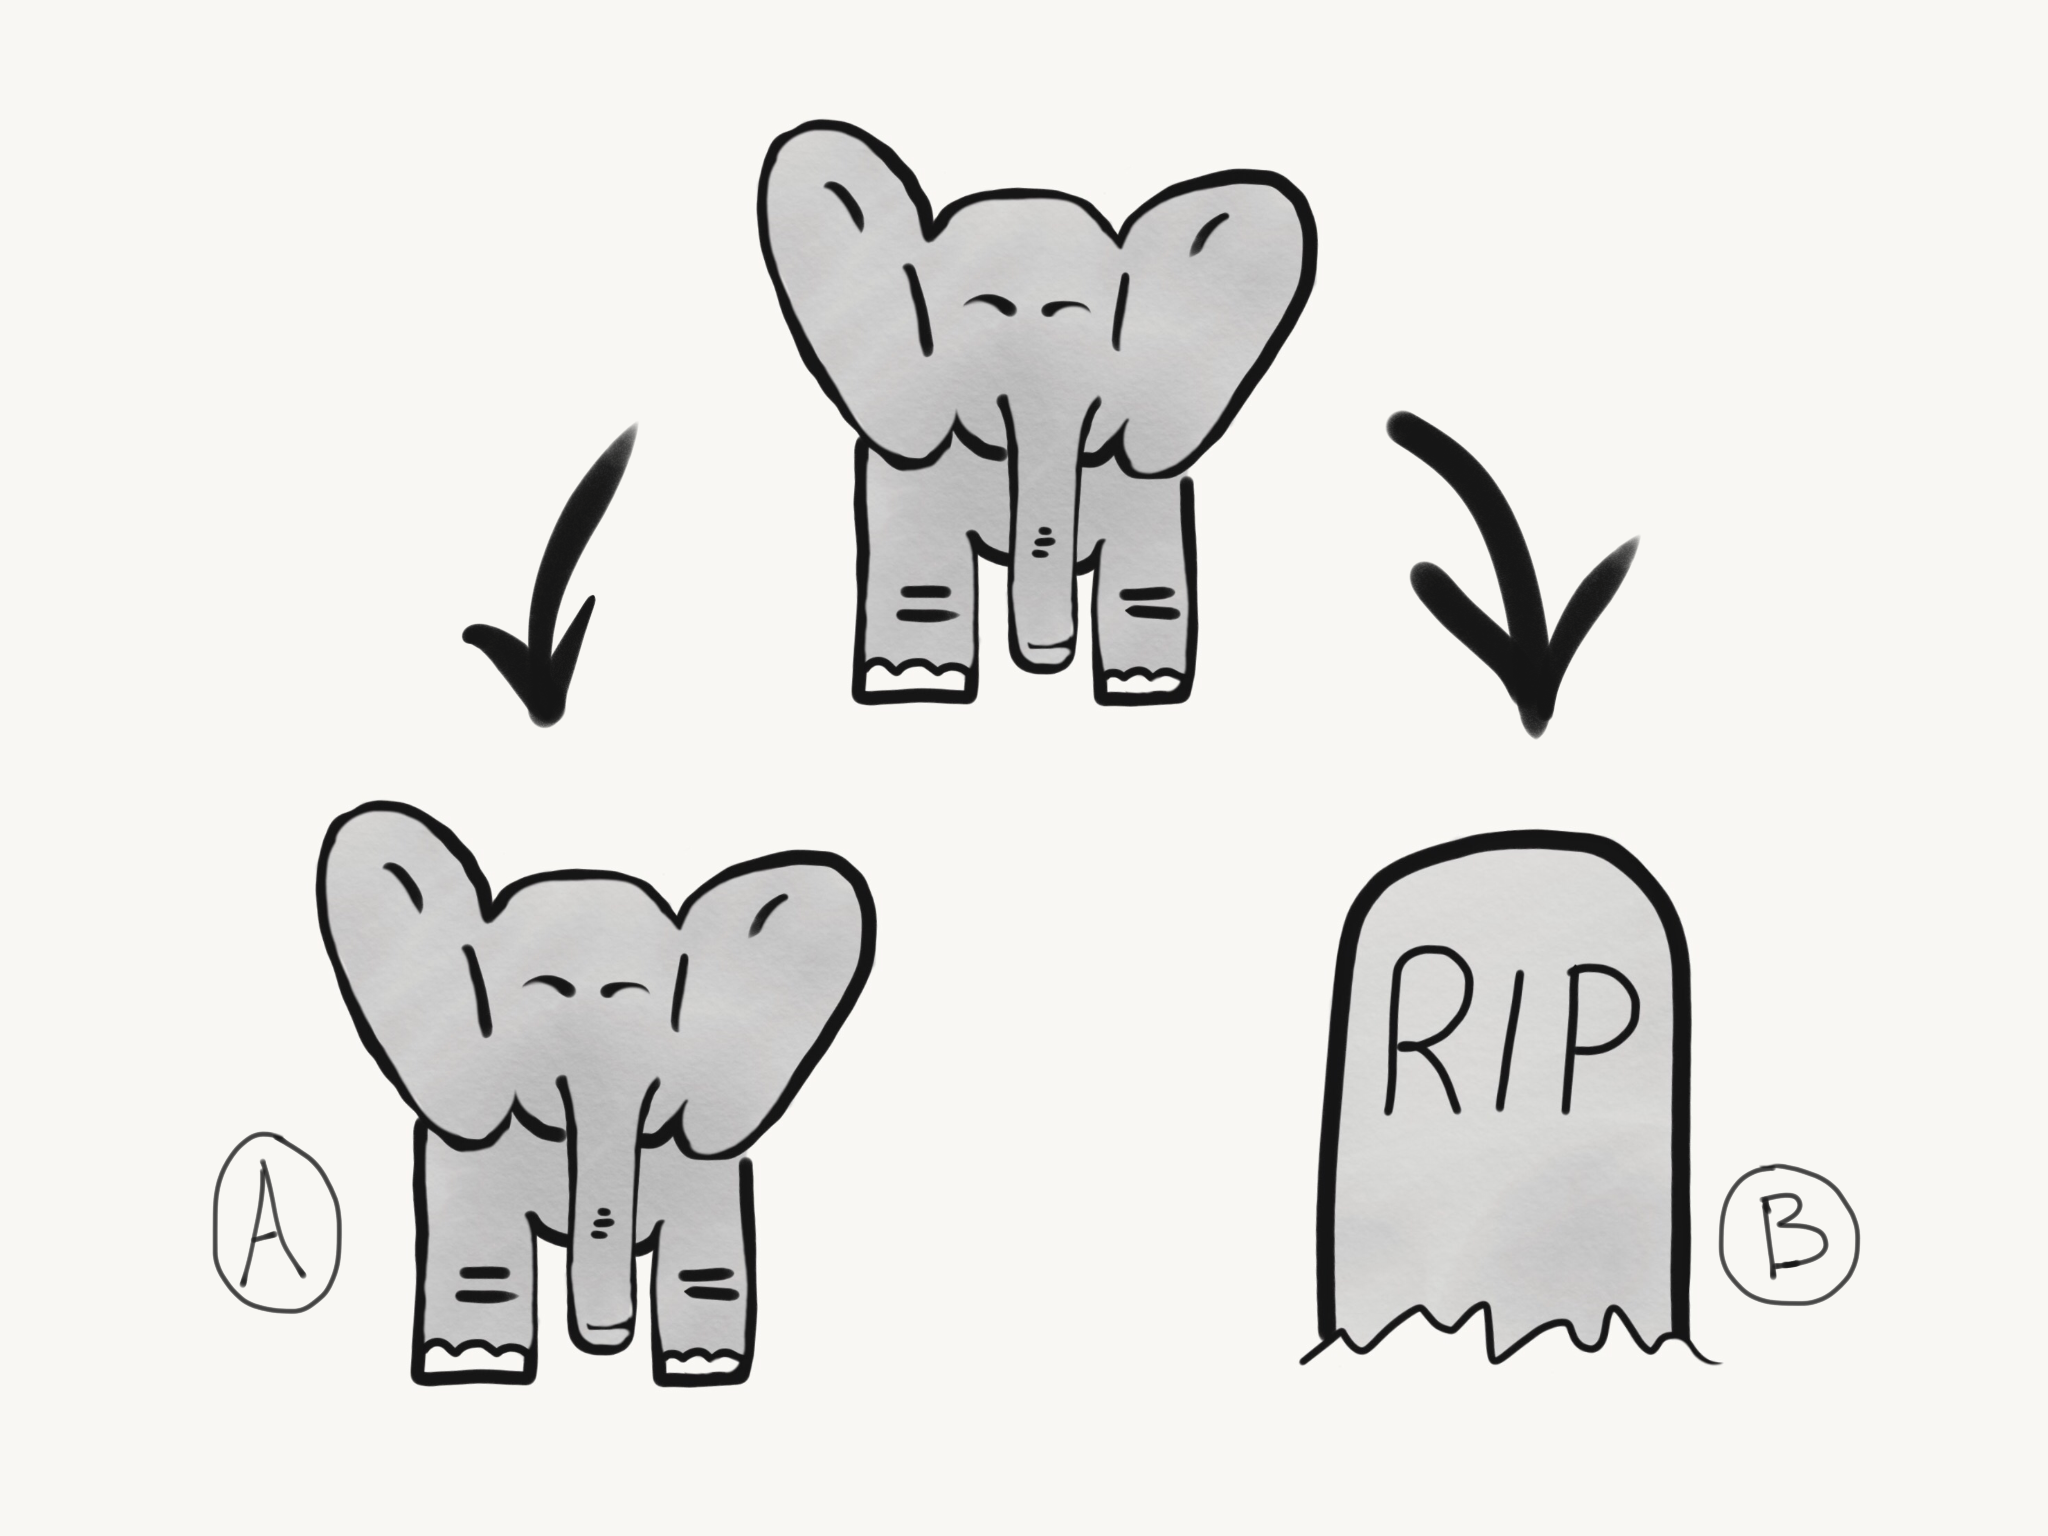
\includegraphics[width=0.8\textwidth]{img/robustness}
 	\captionsetup{singlelinecheck=off,justification=raggedright}
  	\caption{Illustration of robustness; high evolvability left and low evolvability right \cite{Downing2015IntelligenceSystems}.}
    \label{fig:robustness}
\end{figure}
\end{frame}


\section{Organizing and Analyzing Factors that Promote Evolvability}

\begin{frame}{Proximate/Ultimate Thinking}
  \begin{figure}
    \centering
    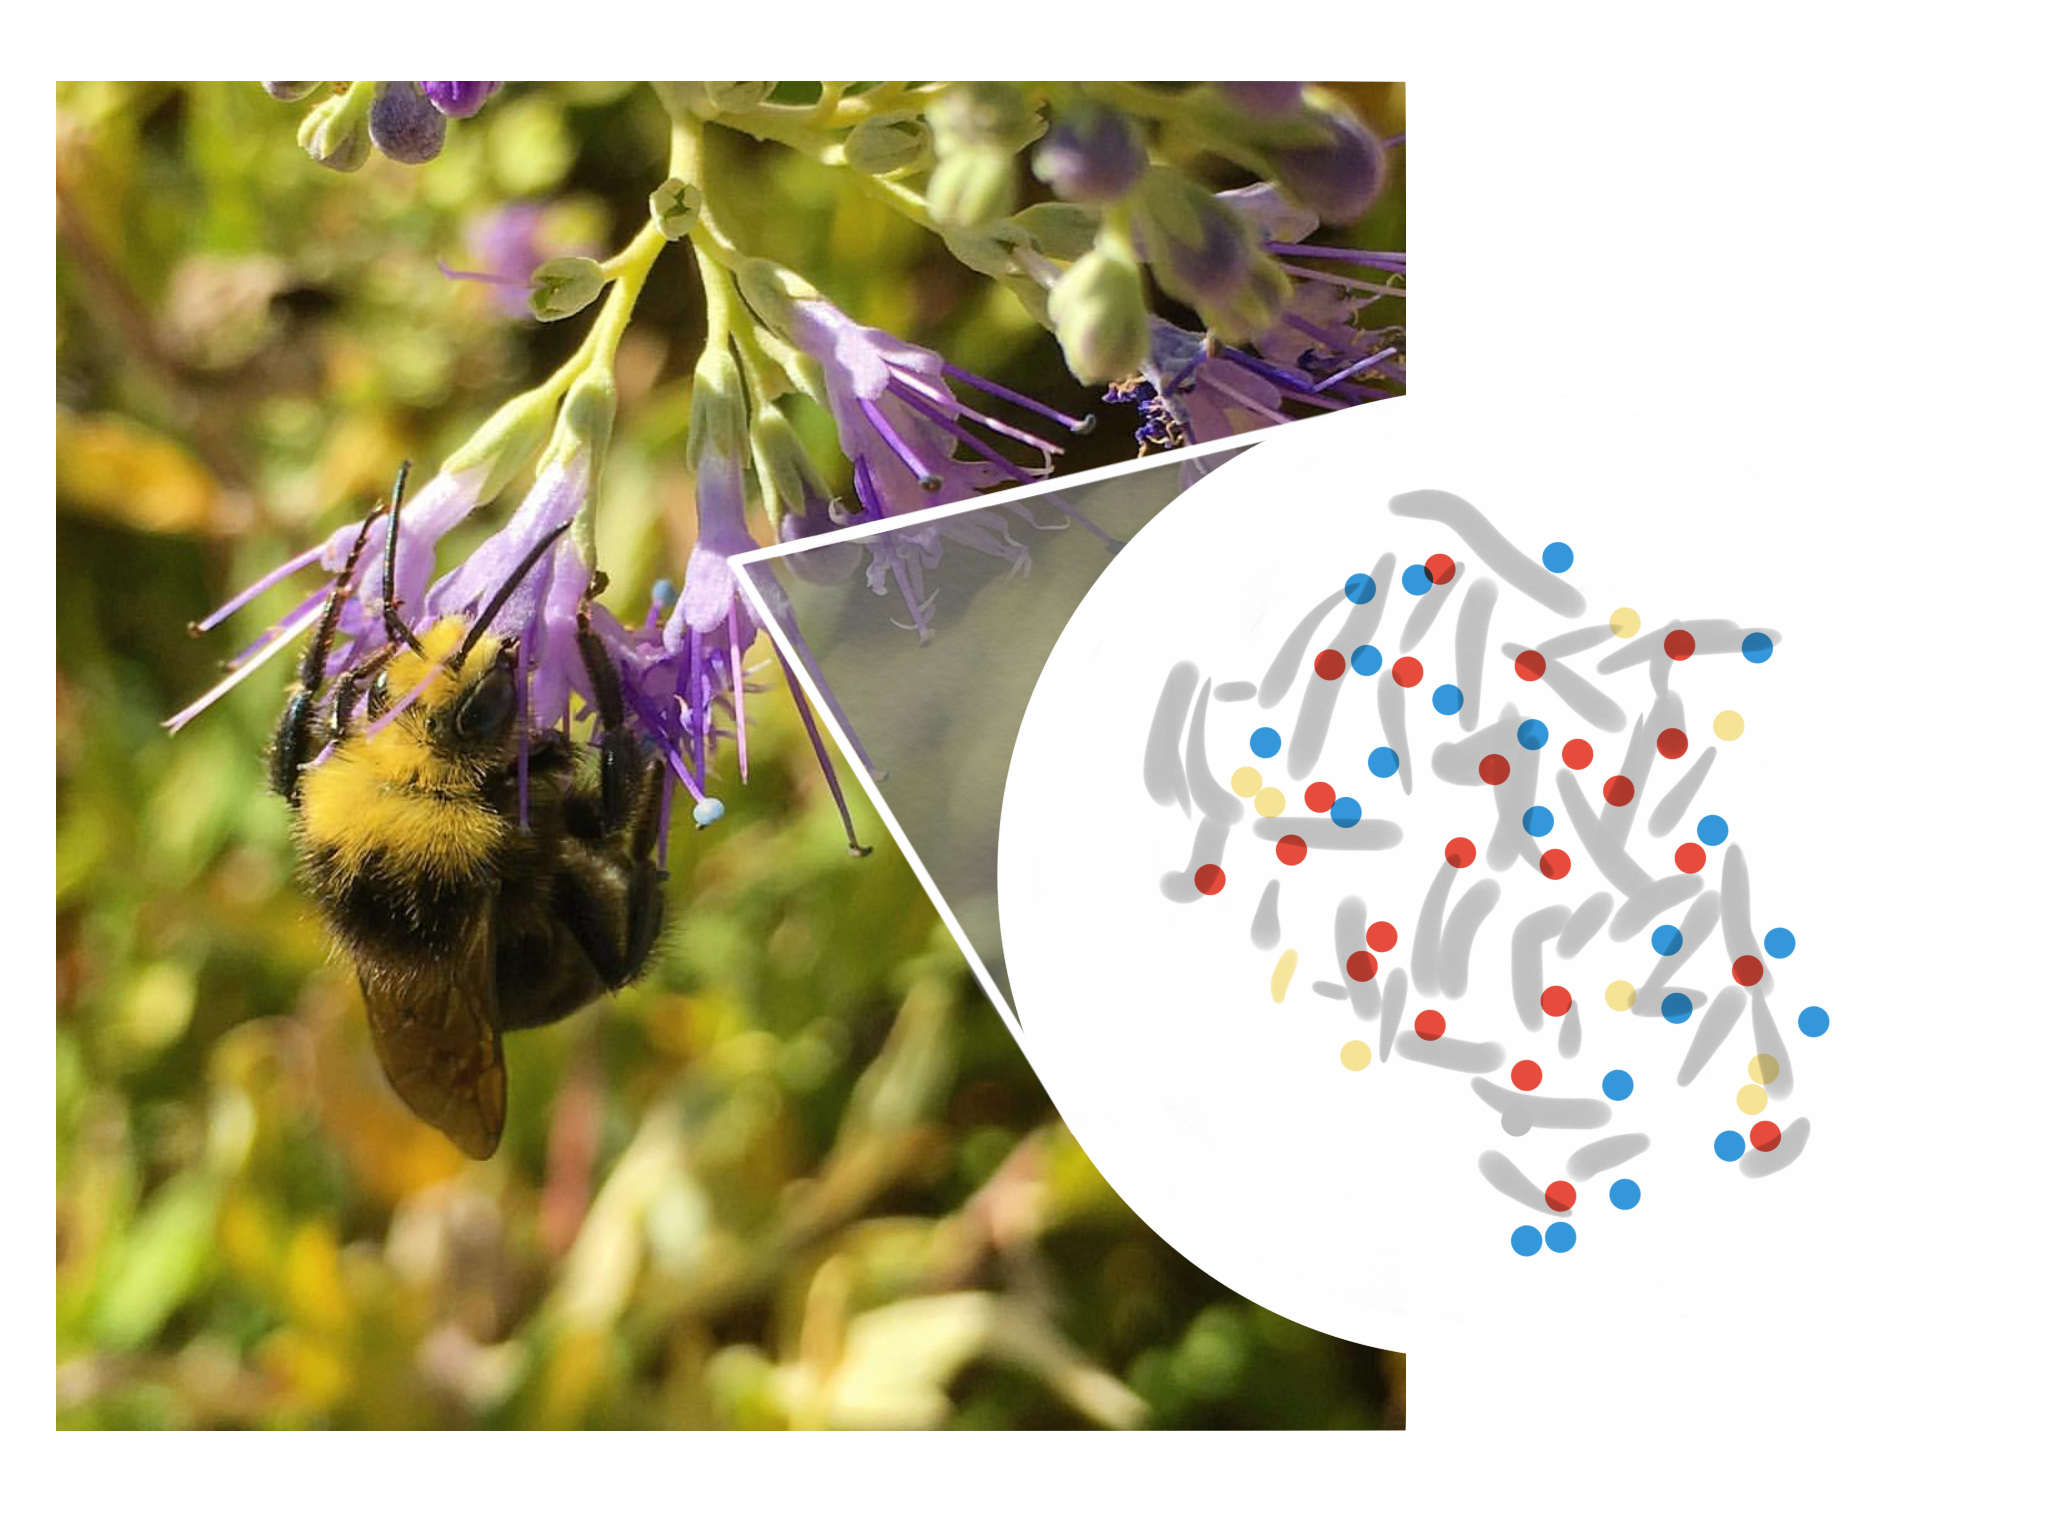
\includegraphics[width=0.8\textwidth]{img/proximate_ultimate}
 	\captionsetup{singlelinecheck=off,justification=raggedright}
  	\caption{Why is the flower purple? Proximate and ultimate explanations differ \cite{Wilson2007EvolutionLives}.}
    \label{fig:proximate_ultimate}
\end{figure}
\end{frame}

\begin{frame}{Proximate/Intermediate/Ultimate Organization}
\textbf{Proximate Causality}
\begin{itemize}
  \item describes specific organismal processes or structures 
\end{itemize}
\textbf{Intermediate Causality}
\begin{itemize}
  \item describes characteristics of an organism as a whole
\end{itemize}
\textbf{Ultimate Causality}
\begin{itemize}
  \item describes the relation between the individual and its environment
\end{itemize}
\end{frame}

\begin{frame}{Proximate/Intermediate/Ultimate Organization}
\begin{columns}[T,onlytextwidth]
\column{0.33\textwidth}
\textbf{Proximate Causality}
\begin{itemize}
  \item duplication and divergence
  \item developmental constraint
  \item hidden genetic variation
  \item exploratory growth
  \item weak linkage
  \item indirect encodings
\end{itemize}
\column{0.33\textwidth}
\textbf{Intermediate Causality}
\begin{itemize}
  \item modularity
  \item robustness
  \item canalization
  \item plasticity
  \item intraindividual degeneracy
  \item interindividual degeneracy
  \item regularity
\end{itemize}
\column{0.33\textwidth}
\textbf{Ultimate Causality}
\begin{itemize}
  \item temporally varying goals
  \item environmental influence on phenotype
  \item fitness degeneracy
\end{itemize}

\end{columns}
\end{frame}

\begin{frame}{Proximal Causality: Developmental Constraint}
  idea: the phenotype results from development, so developmental processes influence the phenotypic outcomes of mutation
    \begin{figure}
\begin{columns}
\begin{column}{0.7\textwidth}
  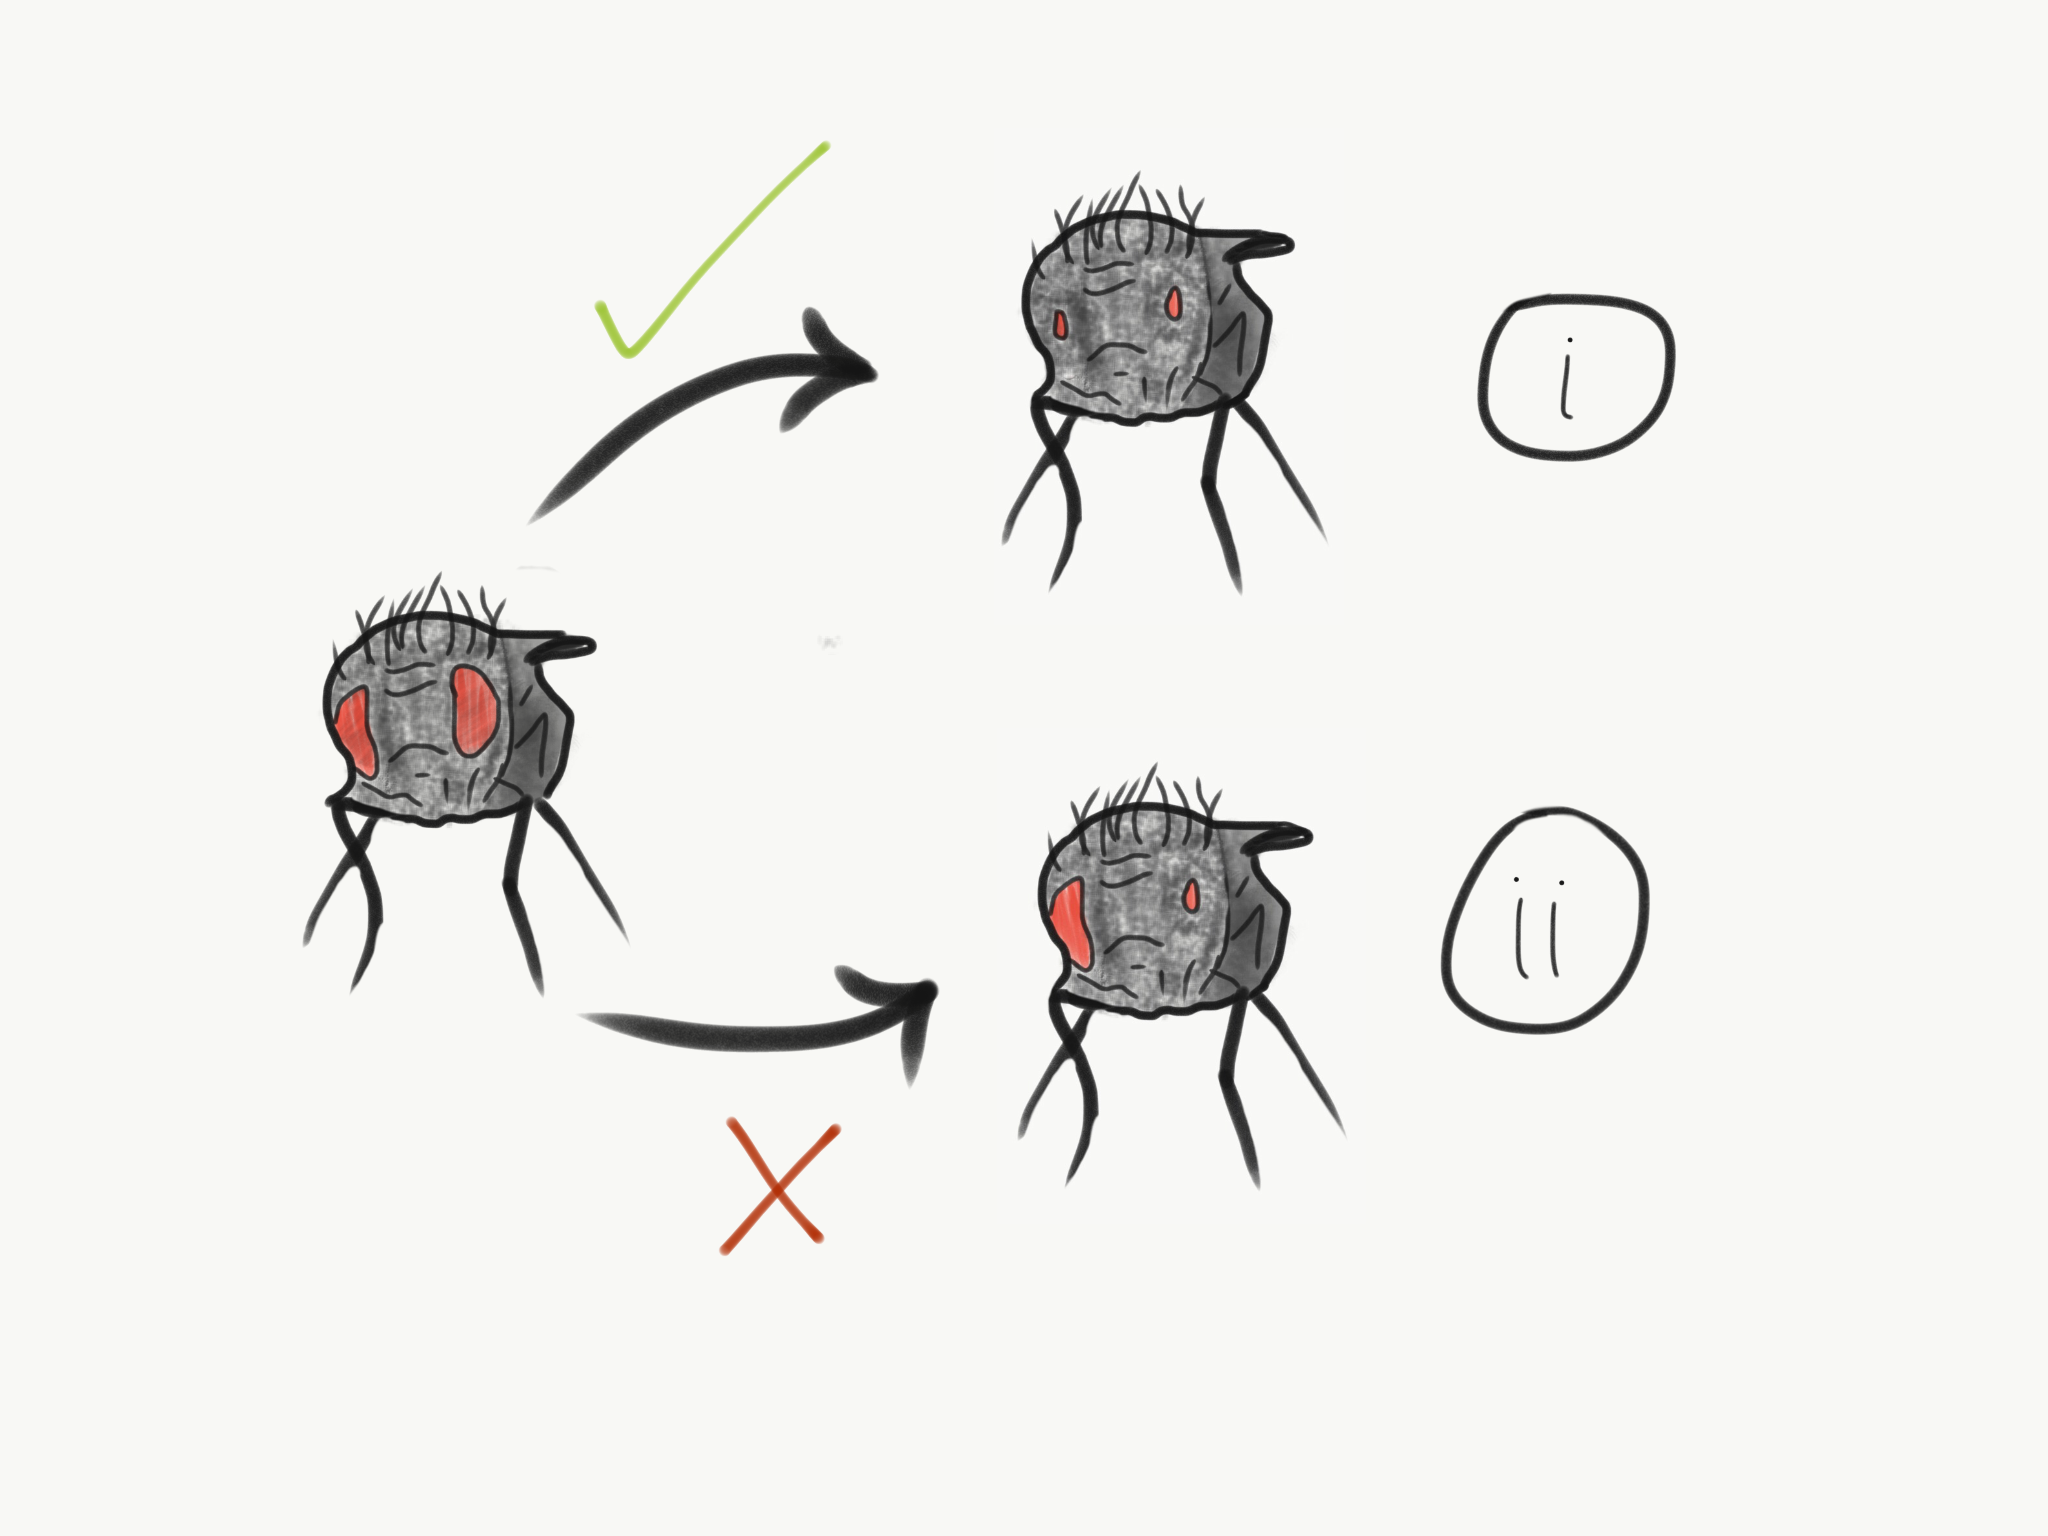
\includegraphics[width=\textwidth]{img/fly_canalization}
 \end{column}
 \begin{column}{0.3\textwidth}
  \caption{Illustration of Canalization Against Bilateral Asymmetry in \textit{Drosophilia melangoster} \cite{Tuinstra1990LackDevelopment}.}
  \label{fig:fly_canalization}
  \end{column}
  \end{columns}
\end{figure}
\end{frame}

\begin{frame}{Intermediate Causality: Intraindividual Degeneracy}
  idea: employing a diverse collection substructures that provide identical or near-identical functionality promote robustness through redundancy while providing many jumping off points for variation through repurposing or elaboration
  \begin{figure}
 \begin{columns}
 \begin{column}{0.6\textwidth}
 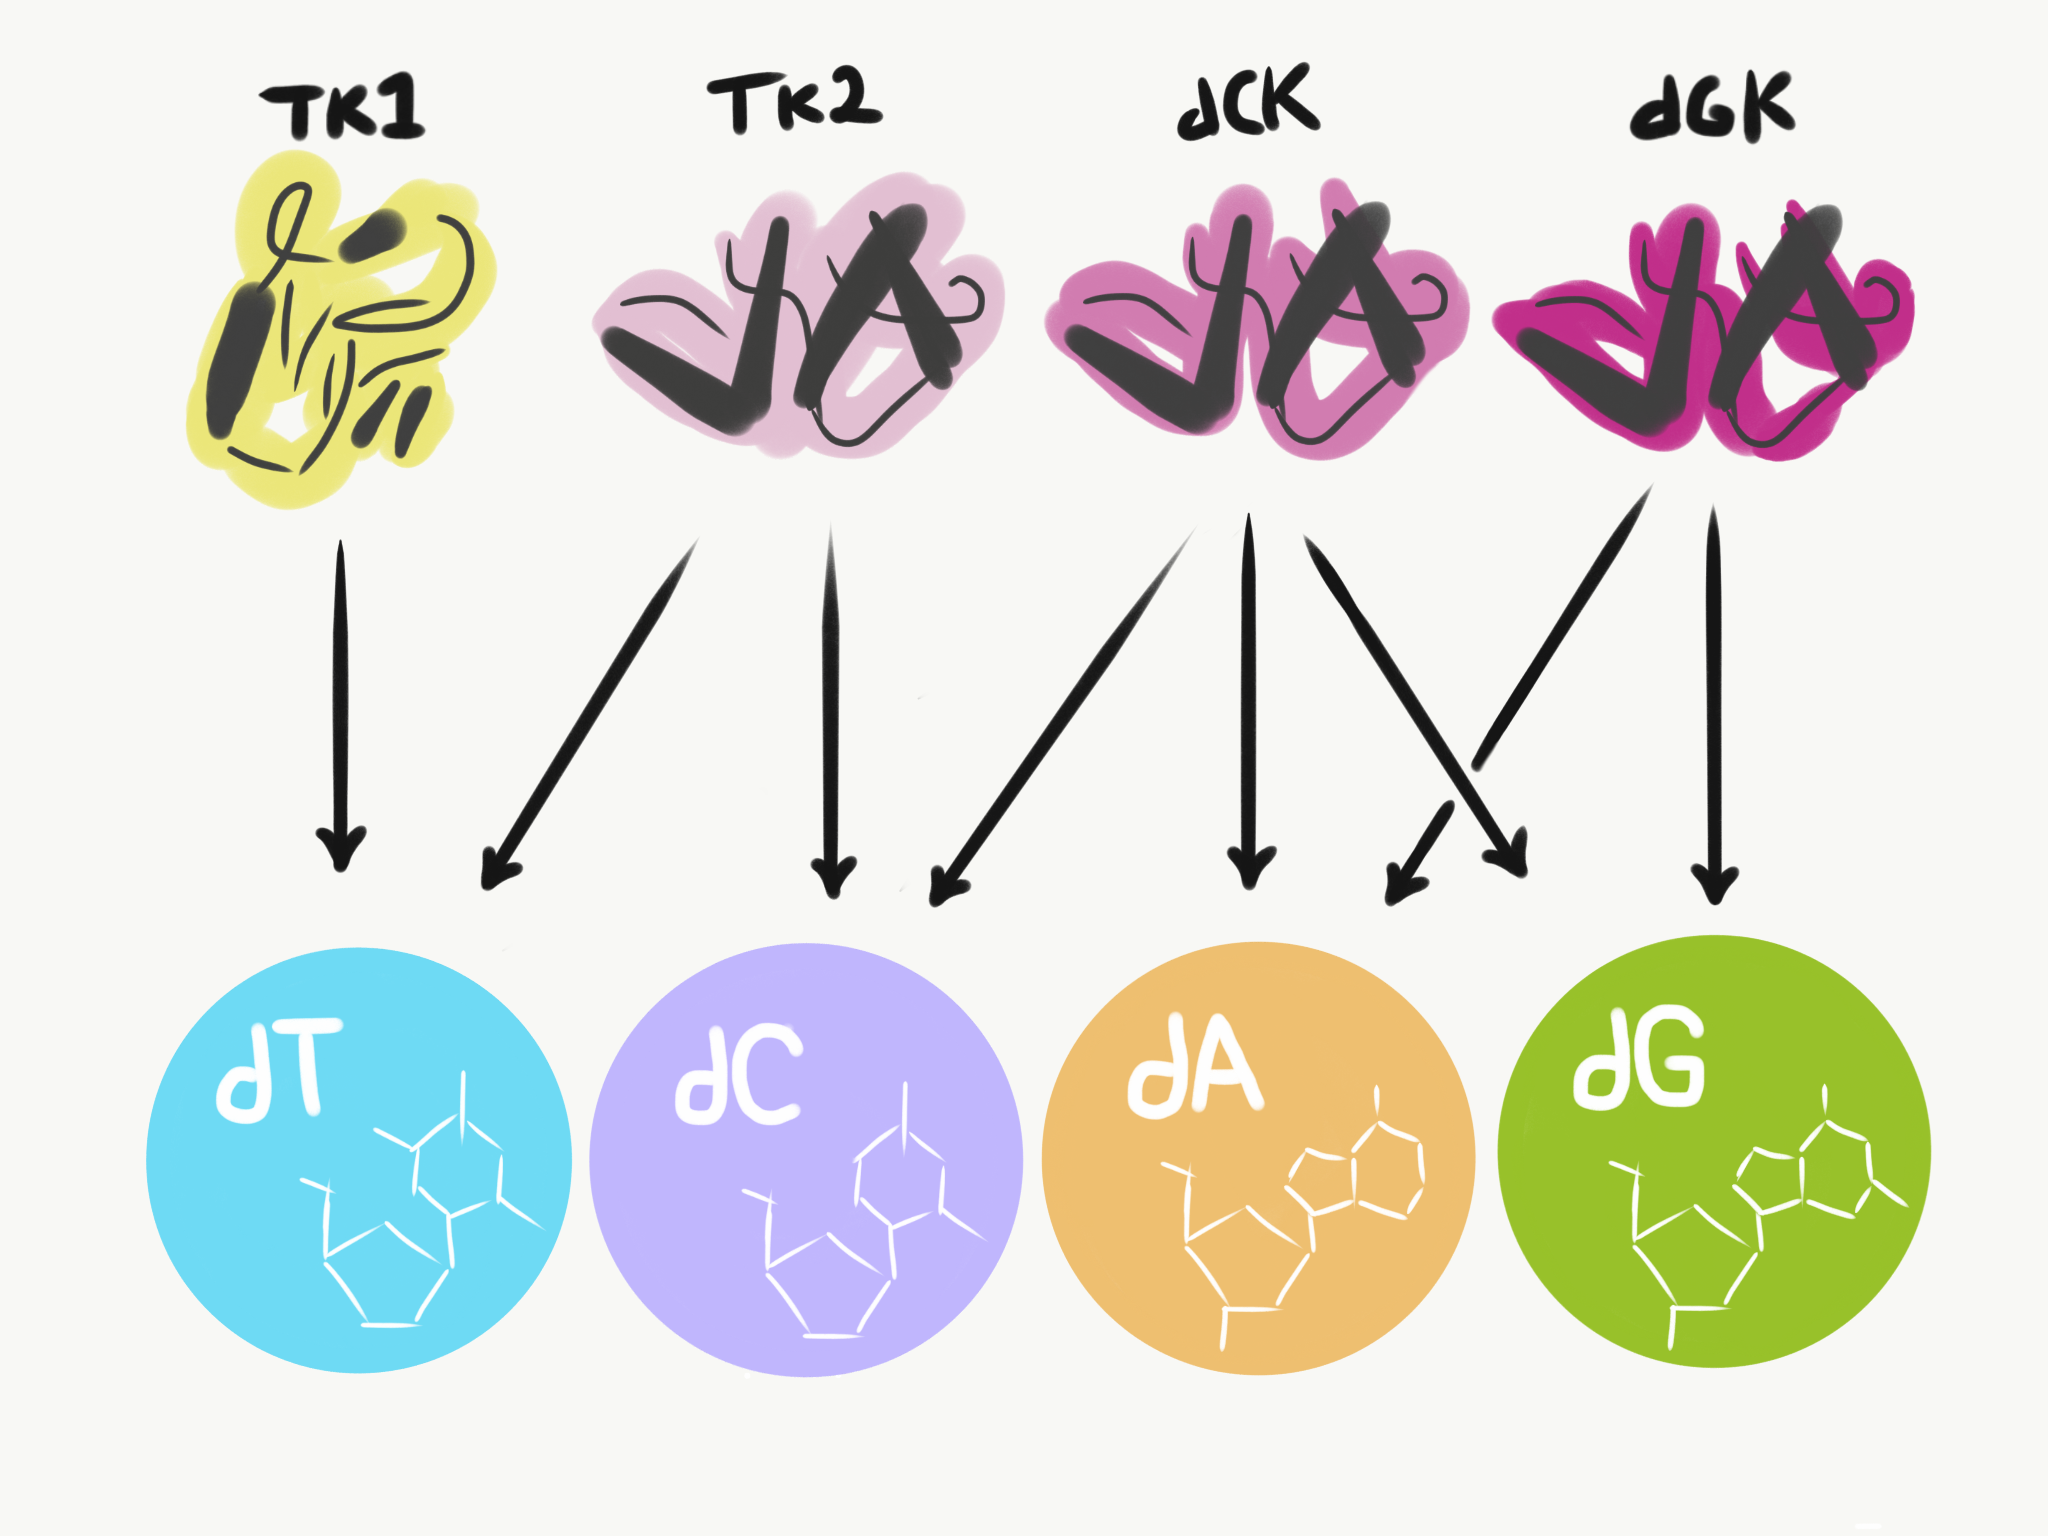
\includegraphics[width=\textwidth]{img/intraindividual_degeneracy}
 \end{column}
 \begin{column}{0.4\textwidth}
\captionsetup{singlelinecheck=off,justification=raggedright}
  	\caption{Mammalian deoxyribonucleoside kinases exhibit degeneracy \cite{Sandrini2005DeoxyribonucleosideReaction.}.}
    \label{fig:intraindividual_degeneracy}
    
\end{column}
\end{columns}
\end{figure}
\end{frame}

\begin{frame}{Ultimate Causality: Modularly Varying Fitness Function}
  idea: if evolution sets a moving target, organisms that produce variable offspring will be selected for 
  \begin{figure}

  \centering
  \begin{columns}[T,onlytextwidth]
\column{\textwidth}
\begin{minipage}[]{0.1\textwidth}
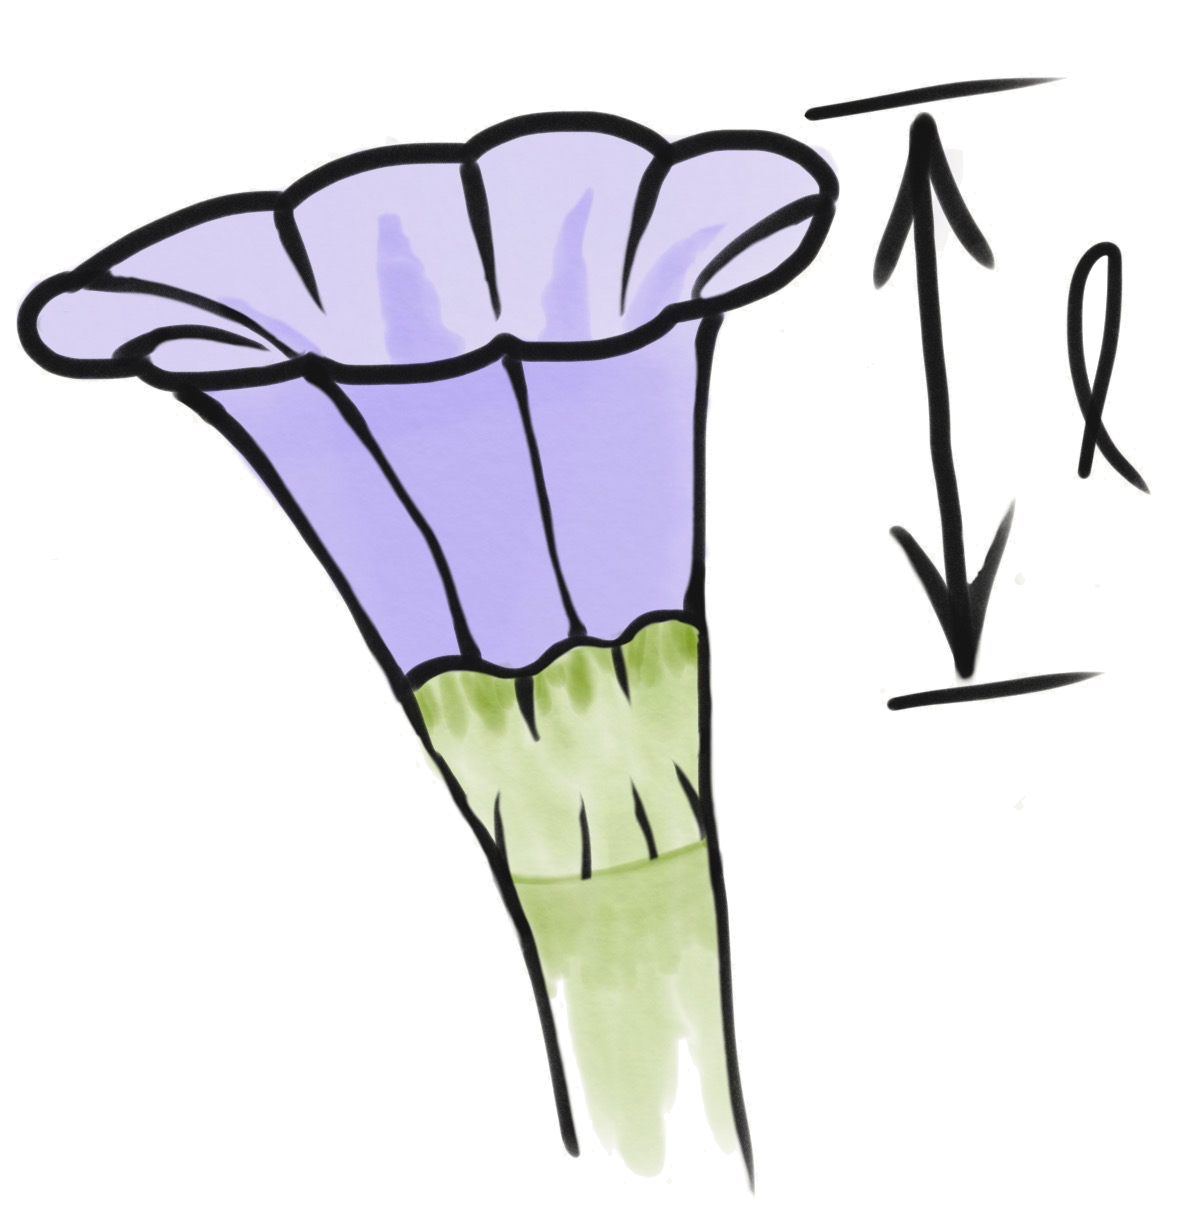
\includegraphics[width=\textwidth]{img/hbird_flower}
\end{minipage}%
\begin{minipage}[]{0.45\textwidth}
   \begin{subfigure}[b]{\textwidth}
    \centering
  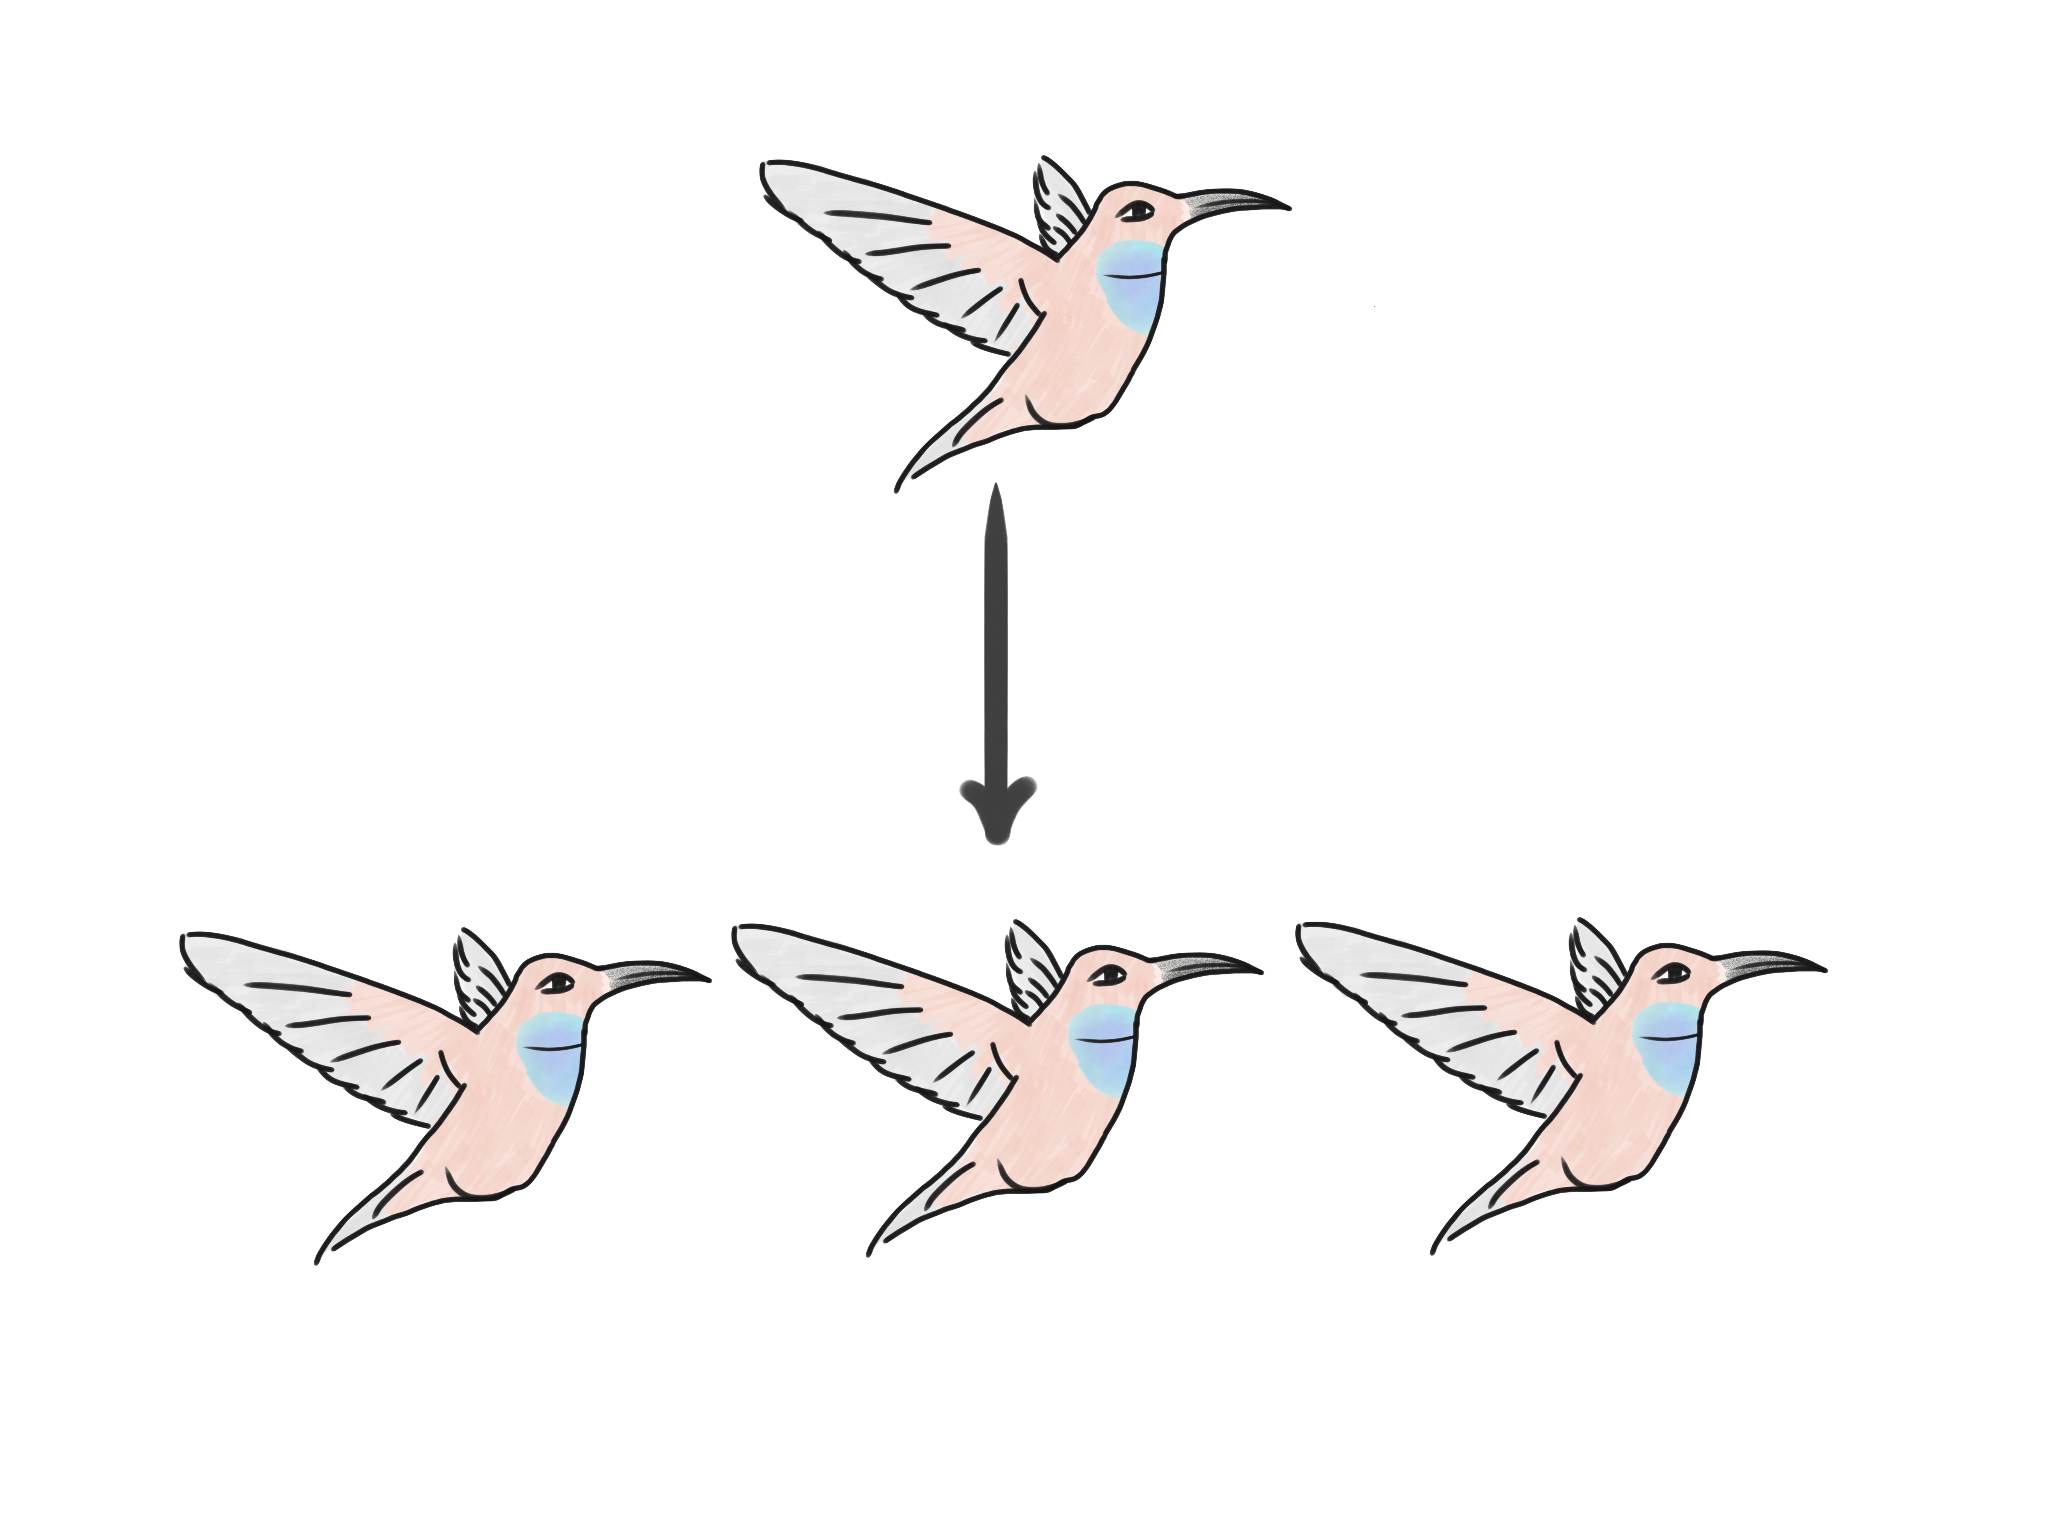
\includegraphics[width=\textwidth]{img/hbird_lowevol}
    \caption{low individual evolvability}
  \end{subfigure}%
\end{minipage}%
\begin{minipage}[]{0.45\textwidth}
\begin{subfigure}[b]{\textwidth}
    \centering
  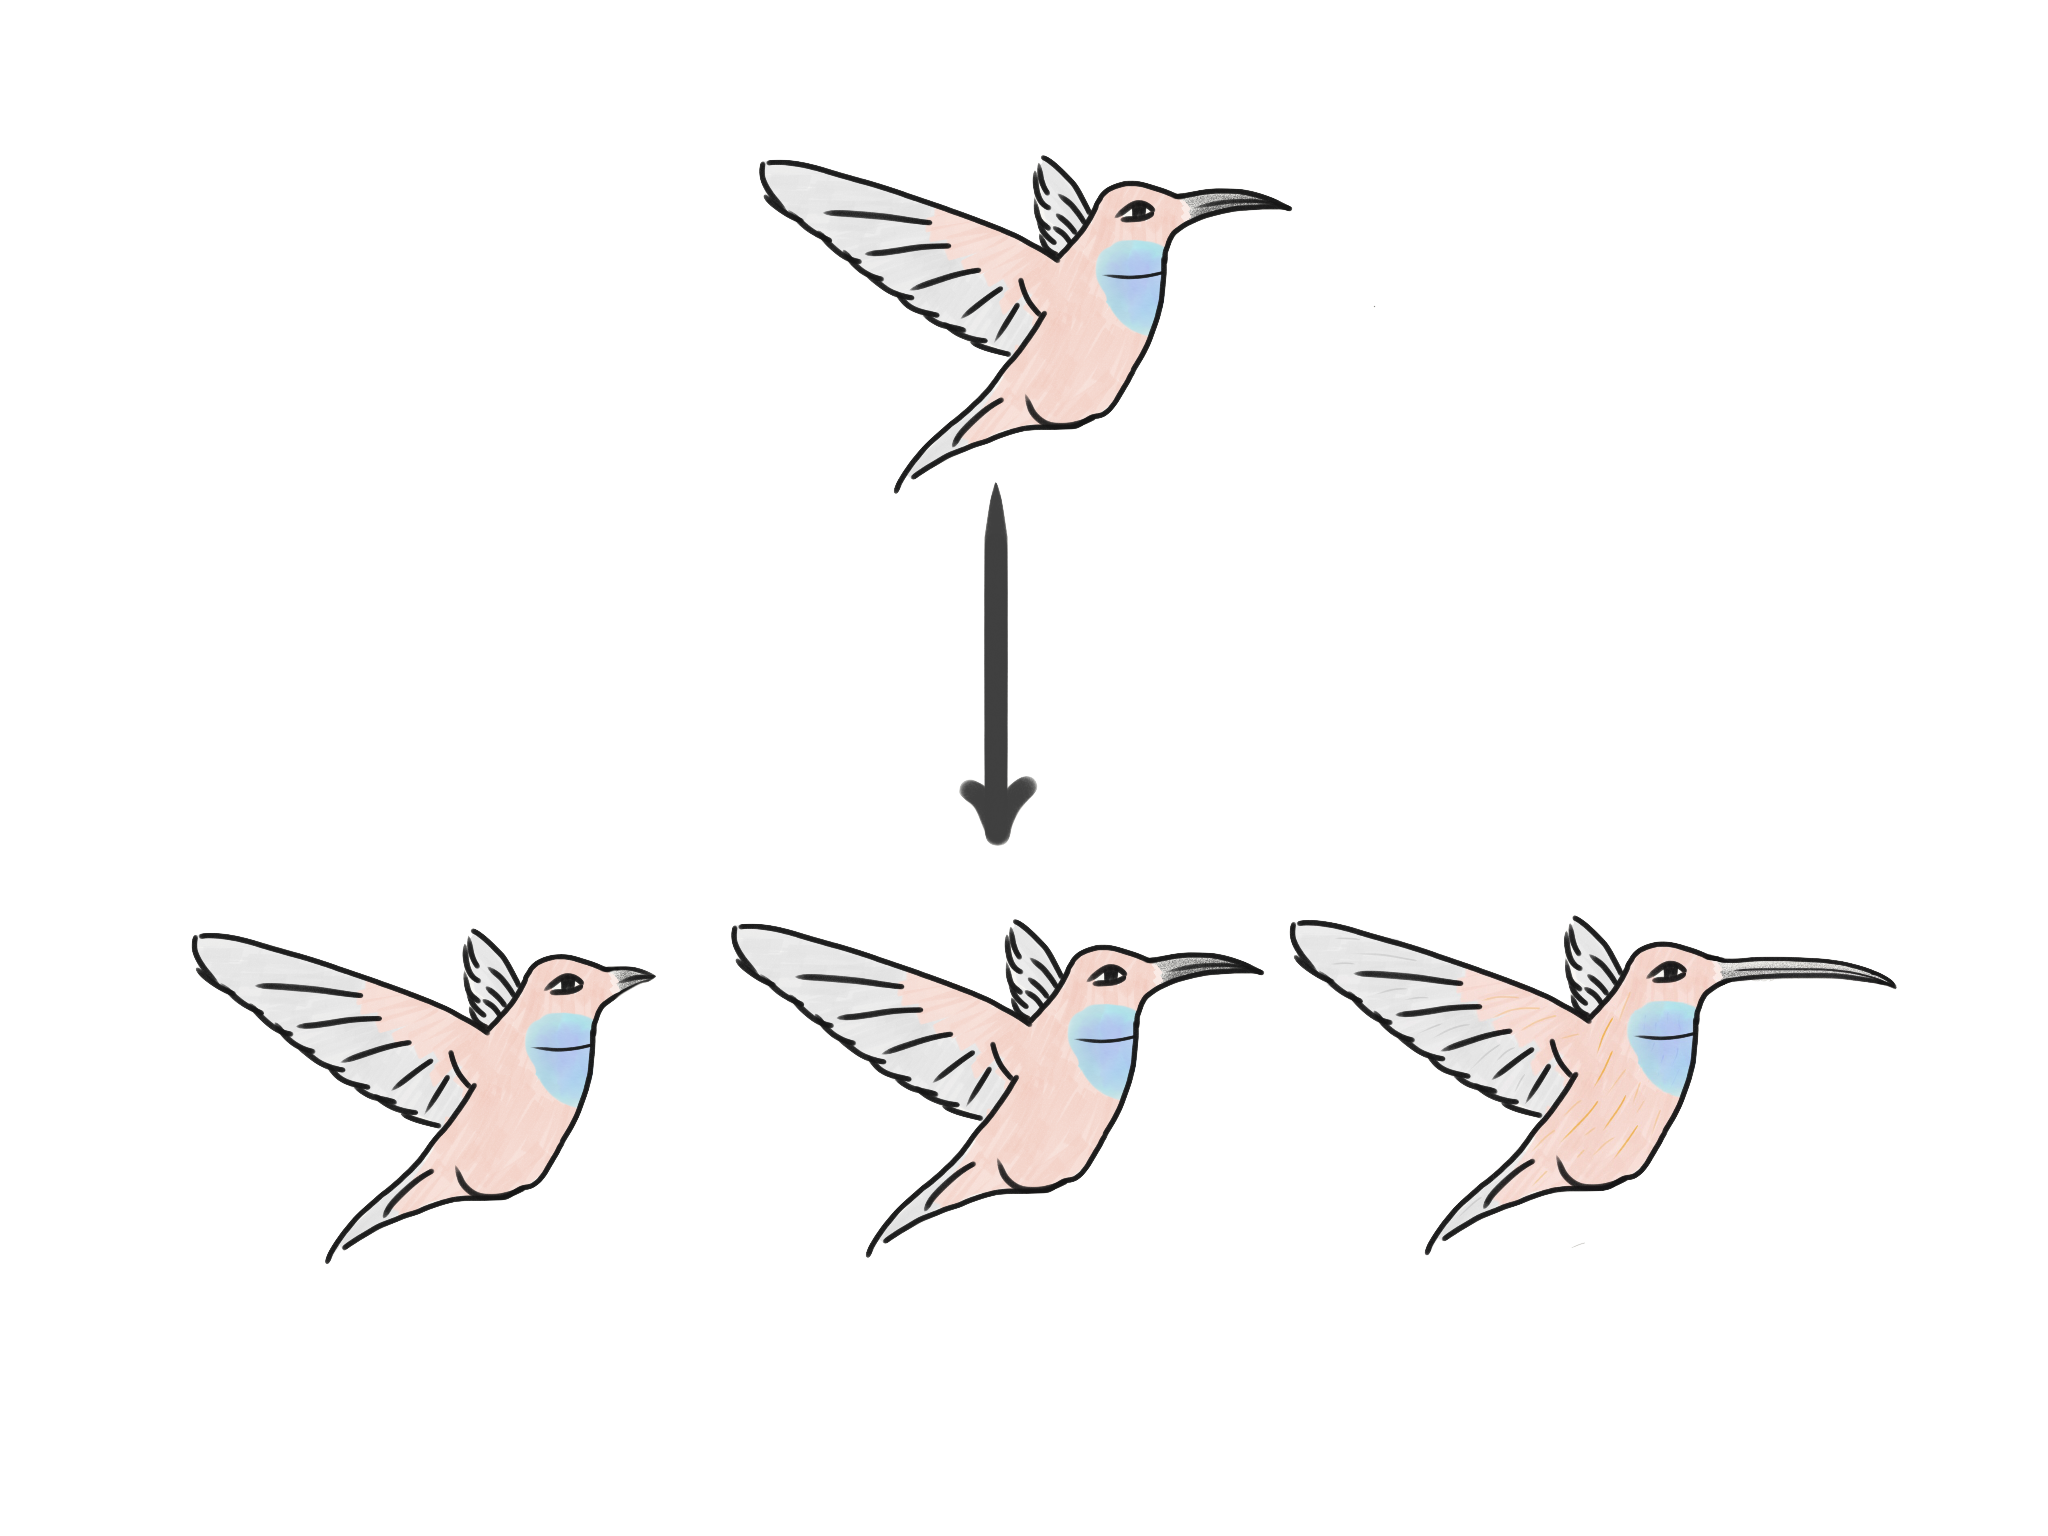
\includegraphics[width=\textwidth]{img/hbird_highevol}
    \caption{high individual evolvability}
  \end{subfigure}
\end{minipage}%
\end{columns}
 
\captionsetup{singlelinecheck=off,justification=raggedright}
  \caption{An hypothetical illustration of a modularly varying fitness function \cite{Kashtan2005SpontaneousMotifs}.}
  \label{fig:hummingbird_selection_pressure}
\end{figure}
\end{frame}

\begin{frame}{Analysis}
\alert{observations:}
\begin{itemize}
  \item proximal and intermediate causality relates to the genotype-phenotype mapping
  \item ultimate causality is related to interaction with the environment to determine fitness
\end{itemize}


\[\downarrow\]

\alert{paths forward:}
\begin{itemize}
\item taking a broader view of fitness and selection 
\item taking a more nuanced view of the developmental process
\end{itemize}
\end{frame}

% \begin{frame}{Analysis}
% \begin{itemize}
%   \item suggests two paths to getting evolvability:
%   \begin{itemize}
%     \item more nuanced artificial developmental process (genotype-phenotype mapping)
%     \item more open-ended selection
%   \end{itemize}
%   \item these paths are already well trod
% \end{itemize}
% \end{frame}

\section{Evolvability in Action}

\begin{frame}{Promoting Evolvability: Indirect Encoding}
  \begin{figure}
  \centering
  \begin{subfigure}[b]{0.5\textwidth}
    \centering
    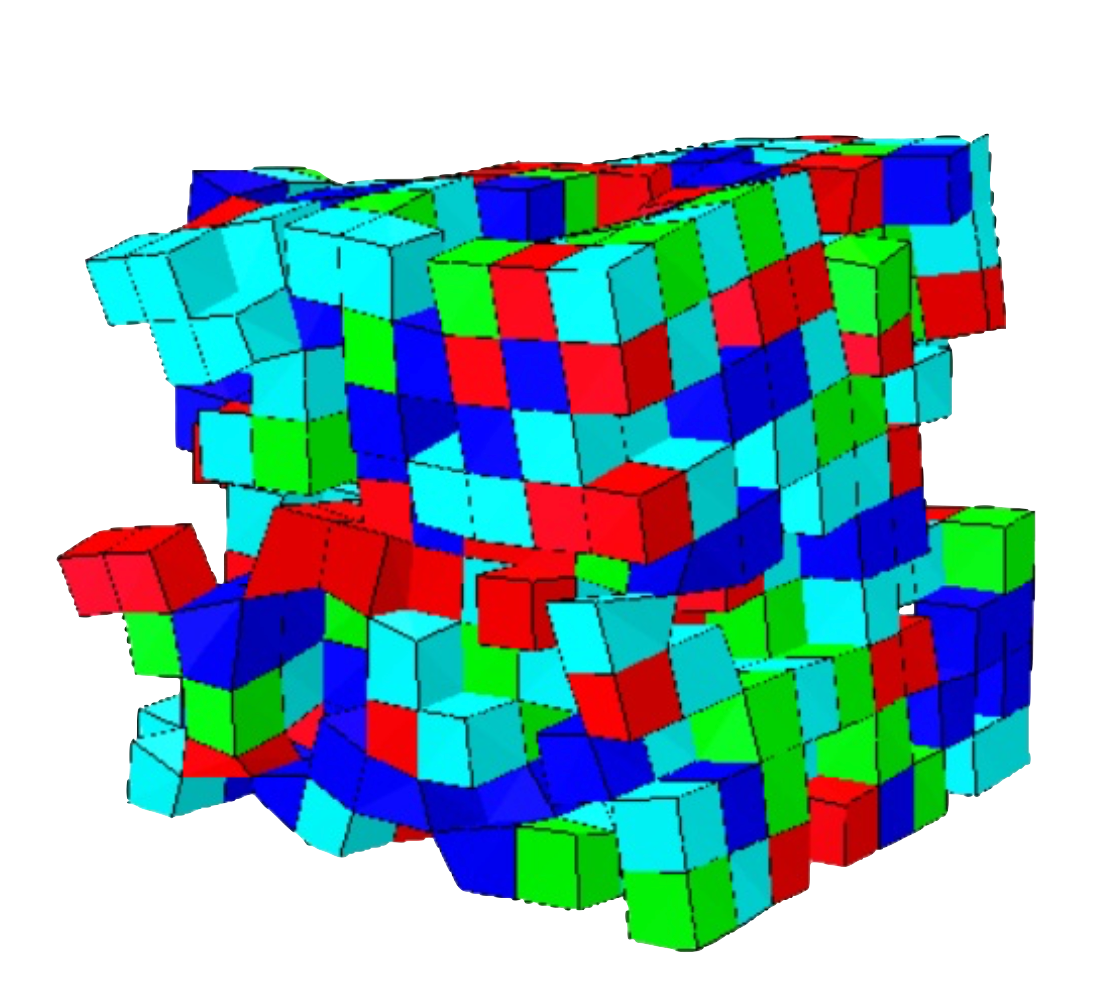
\includegraphics[width=\textwidth]{img/direct_encoding.png}
    \caption{direct encoding (low regularity)}
    \label{subfig:canalization}
  \end{subfigure}%
  \hfill
  \begin{subfigure}[b]{0.5\textwidth}
    \centering
    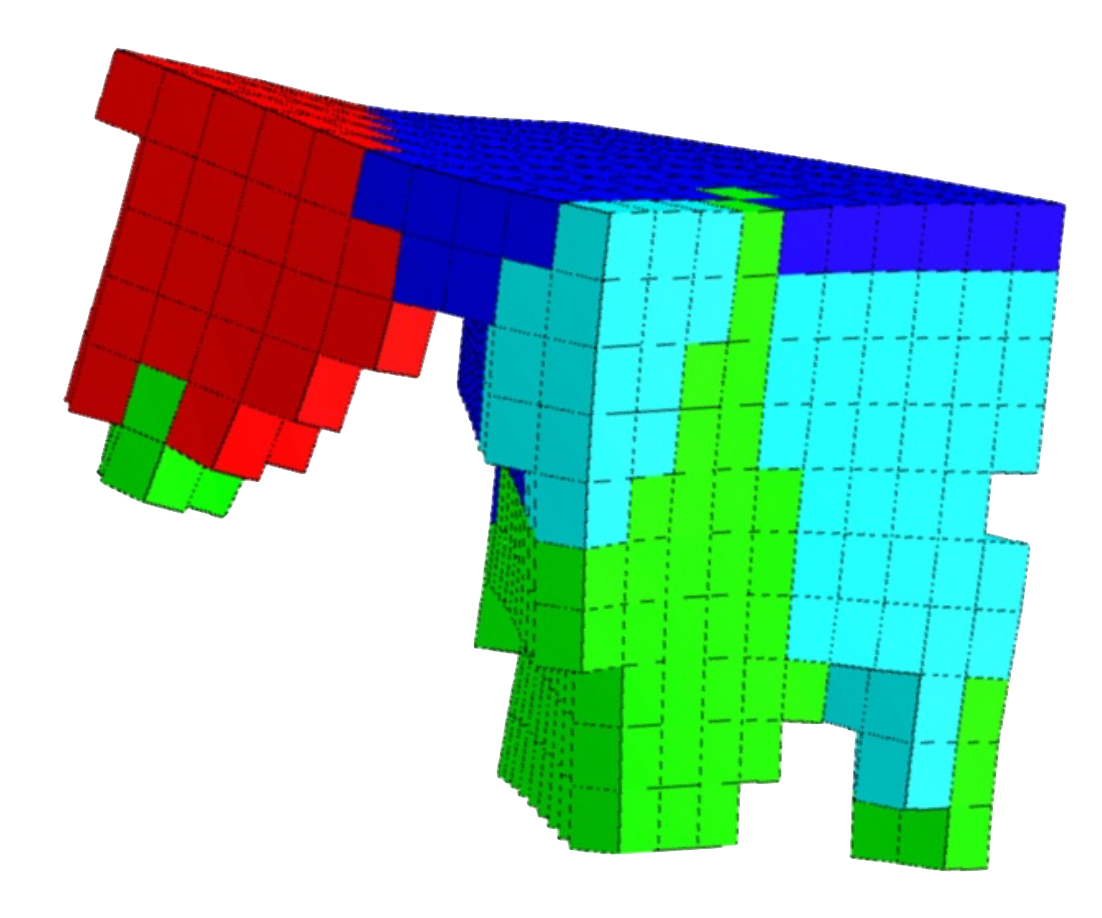
\includegraphics[width=\textwidth]{img/cppn-neat_encoded.png}
    \caption{indirect encoding (high regularity)}
  \end{subfigure}
  \captionsetup{singlelinecheck=off,justification=raggedright}
  \caption{Representative examples of soft robots evolved with direct and indirect representations \cite[Figures 6, 7]{Cheney2013UnshacklingEncoding}}
  \label{fig:direct_irregular_vs_indirect_regular}
\end{figure}
\end{frame}

\begin{frame}{Promoting Evolvability: Fitness Niches}
	\begin{figure}
\begin{center}
\label{fig:cppn_images}
  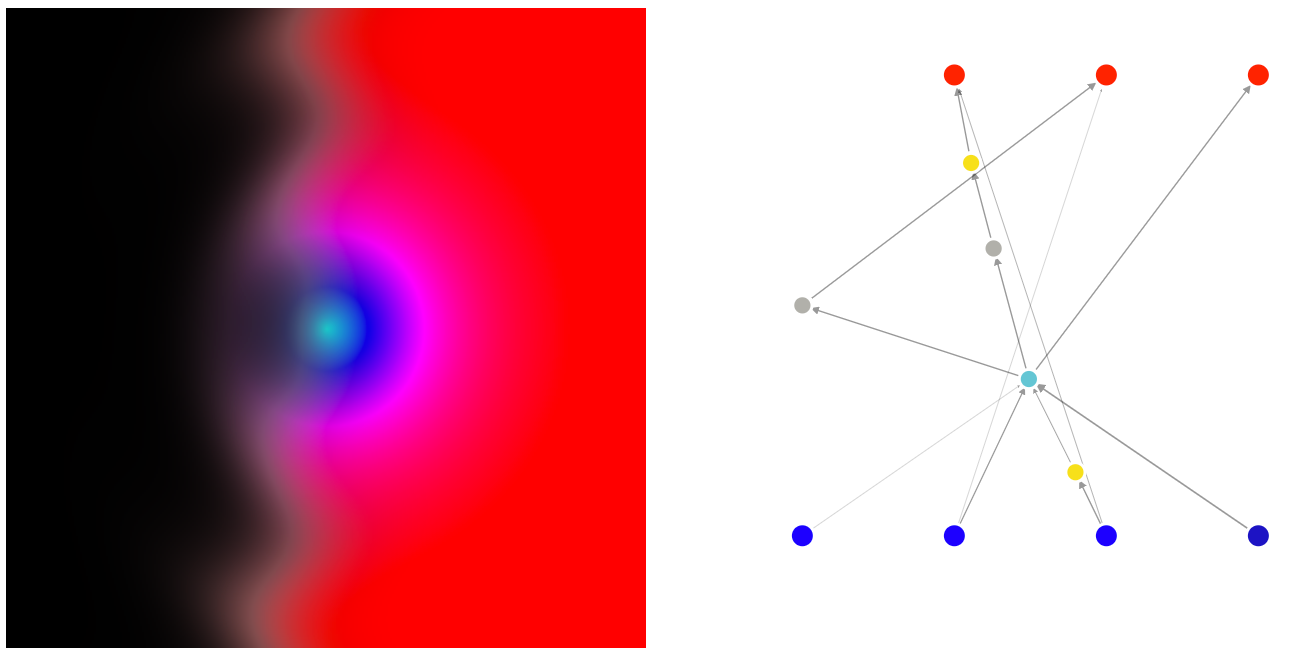
\includegraphics[width=0.4\textwidth]{img/parent} \\
  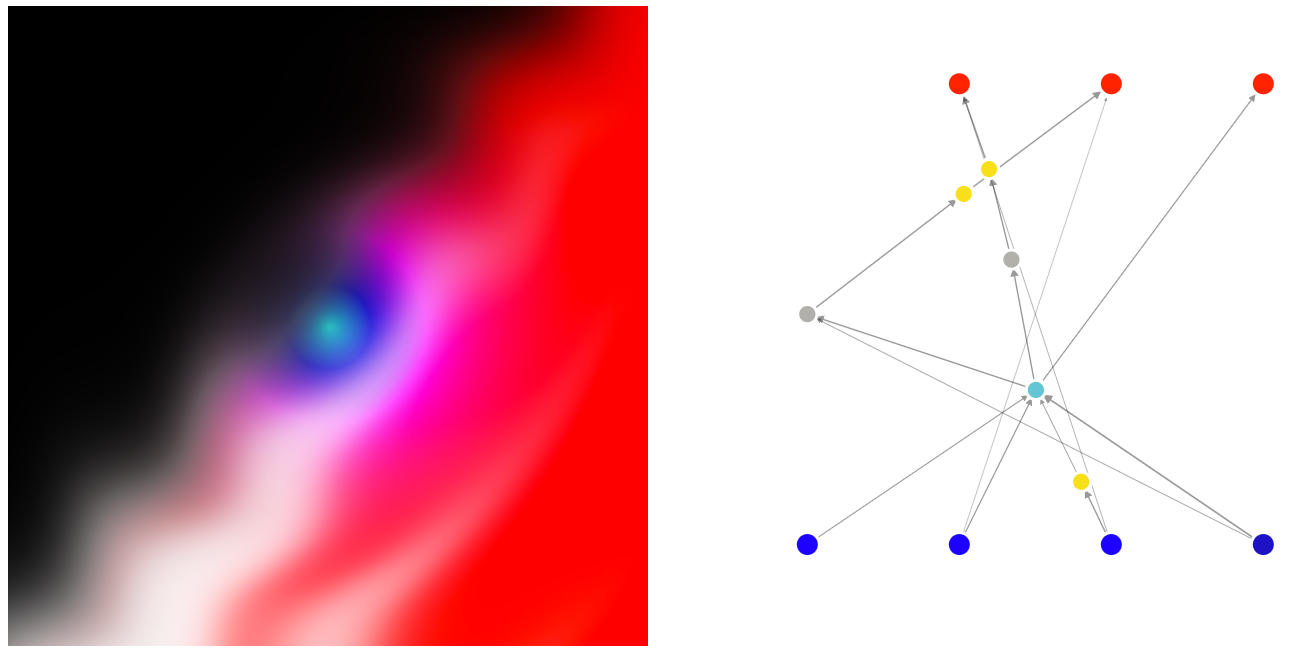
\includegraphics[width=0.4\textwidth]{img/offspring} \\
  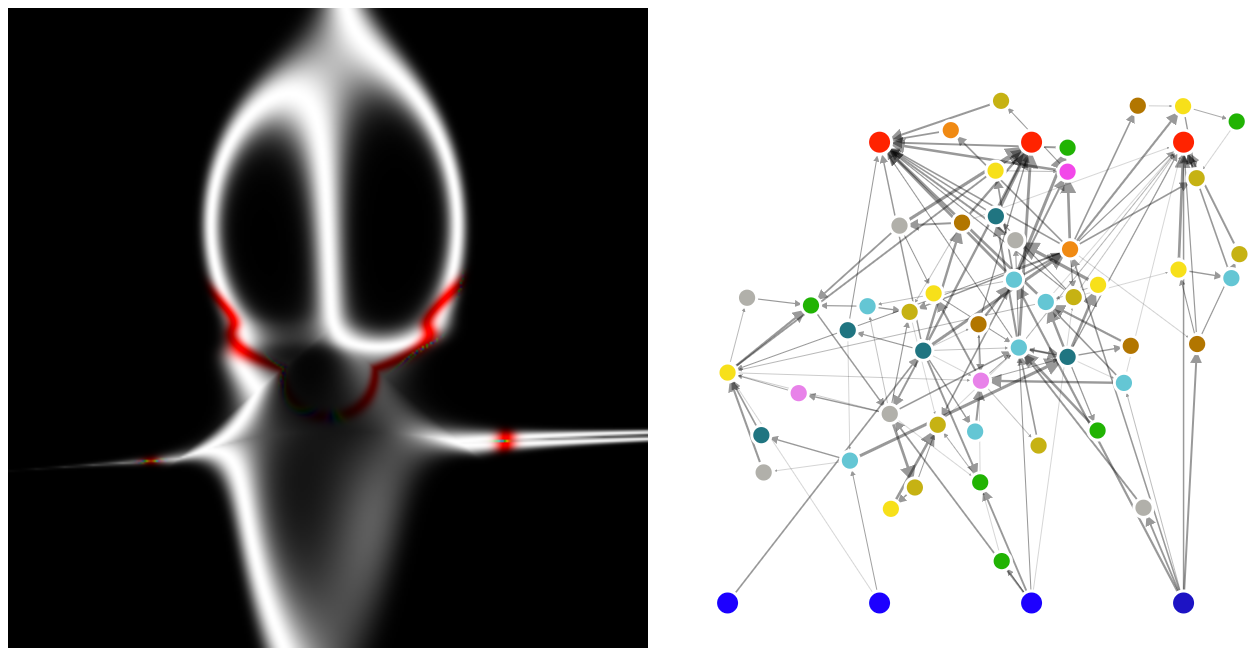
\includegraphics[width=0.4\textwidth]{img/better_goast}
  \end{center}
  \captionsetup{singlelinecheck=off,justification=raggedright}

  \caption{Illustration of compositional pattern producing networks (right) and their output images (left) generated via \cite{Ha2015Neurogram}.}
\end{figure}
\end{frame}

\begin{frame}{Promoting Evolvability: Fitness Niches}
\vfill
	\begin{figure} \label{fig:dnn}
  \begin{center}
  
\includegraphics[width=0.5\textwidth]{img/recognize} \\
  
\includegraphics[width=0.5\textwidth]{img/confused}
  \end{center}
  \captionsetup{singlelinecheck=off,justification=raggedright}

  \caption{A deep neural network (DNN) is trained to recognize a specific category of images.}
\end{figure}
    \vfill
\end{frame}

\begin{frame}{Promoting Evolvability: Fitness Niches}
\vspace{2ex}
	\begin{figure}
    \centering
  \begin{columns}
  \begin{column}{0.6\textwidth}
  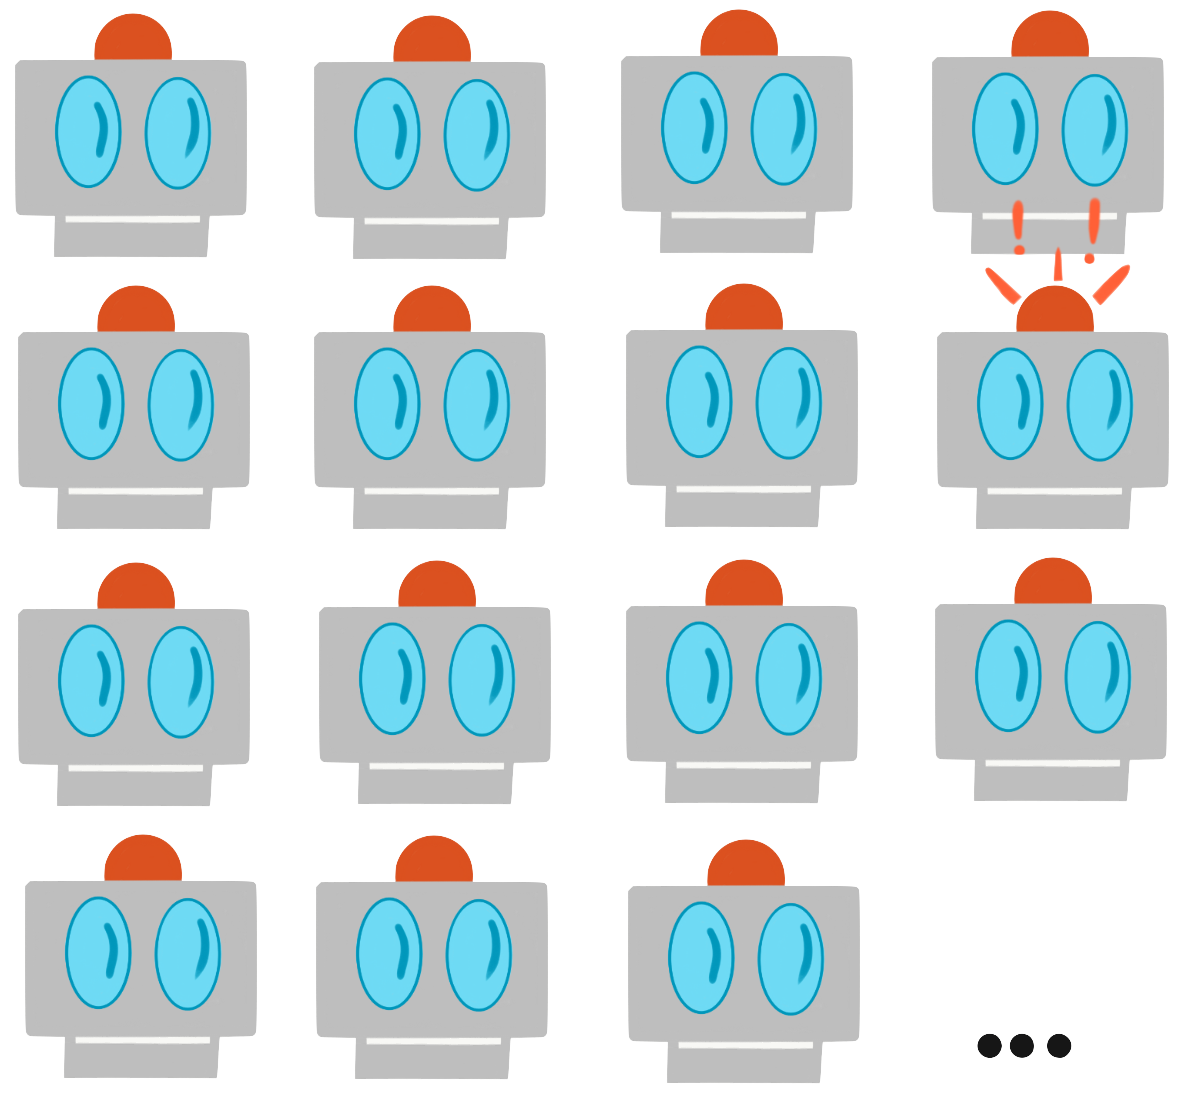
\includegraphics[width=0.9\textwidth]{img/dnn_collection}
   \end{column}
   \begin{column}{0.4\textwidth}
   
\includegraphics[width=0.9\textwidth]{img/cat}
   \end{column}
	\end{columns}
\captionsetup{singlelinecheck=off,justification=raggedright}
  	\caption{Several hundred fitness niches are defined using DNNs each trained to recognize different categories \cite{Nguyen2015InnovationLearning}.}
    \label{fig:niches}
\end{figure}
\end{frame}

\begin{frame}{Promoting Evolvability: Fitness Niches}
\vspace{2ex}	
\begin{figure}
    \centering
    \begin{columns}
    \begin{column}{0.7\textwidth}
     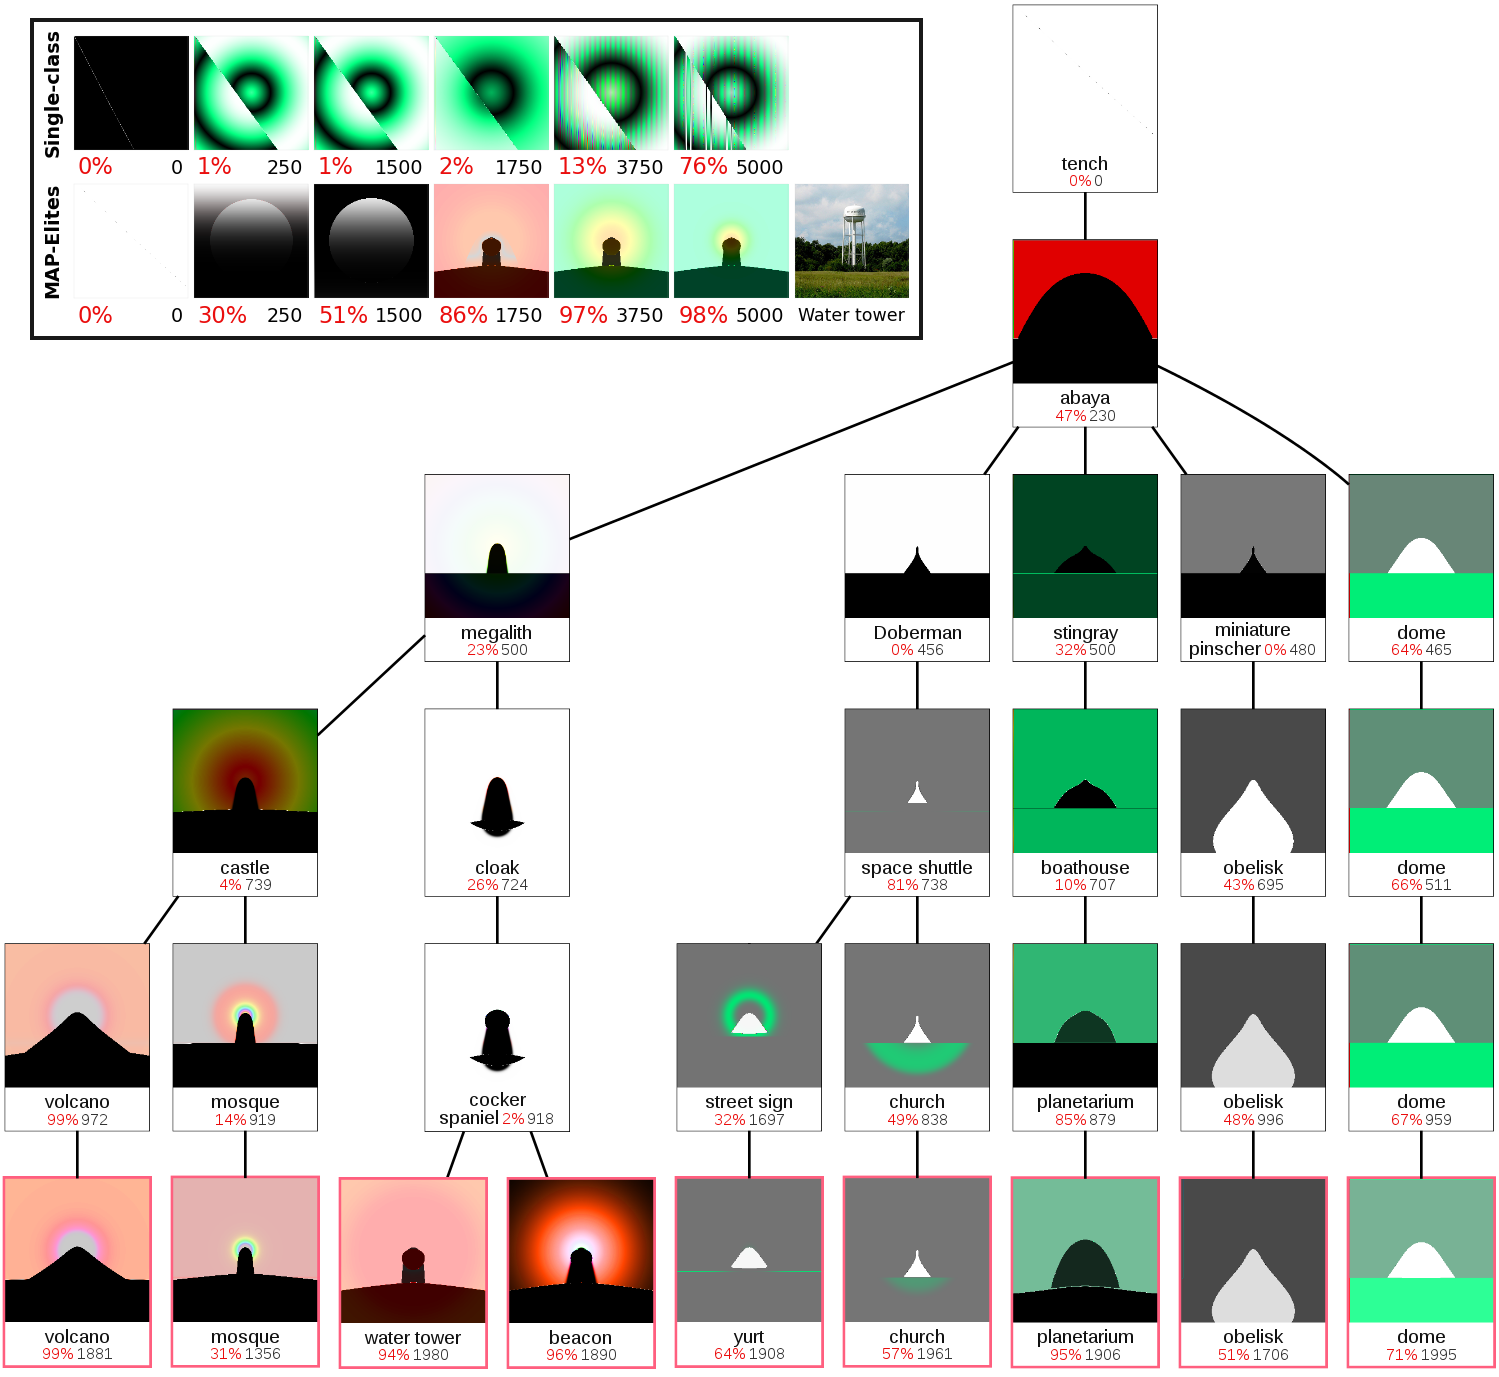
\includegraphics[width=\textwidth]{img/ie_phylogenetic_tree_combined}
    \end{column}
    \begin{column}{0.3\textwidth}
   	\captionsetup{singlelinecheck=off,justification=raggedright}
  	\caption{An illustration of goal-switching, where offspring from a parent that occupies one niche invade another \cite[Figure 9]{Nguyen2015InnovationLearning}. Individuals that promote phenotypically variable offspring are rewarded \cite{Mengistu2016EvolvabilityIt}.}
    \label{fig:goal_switching}
    \end{column}
    \end{columns}
   

\end{figure}
\end{frame}

\begin{frame}{Promoting Evolvability: Fitness Niches}
	\begin{figure}
    \centering
    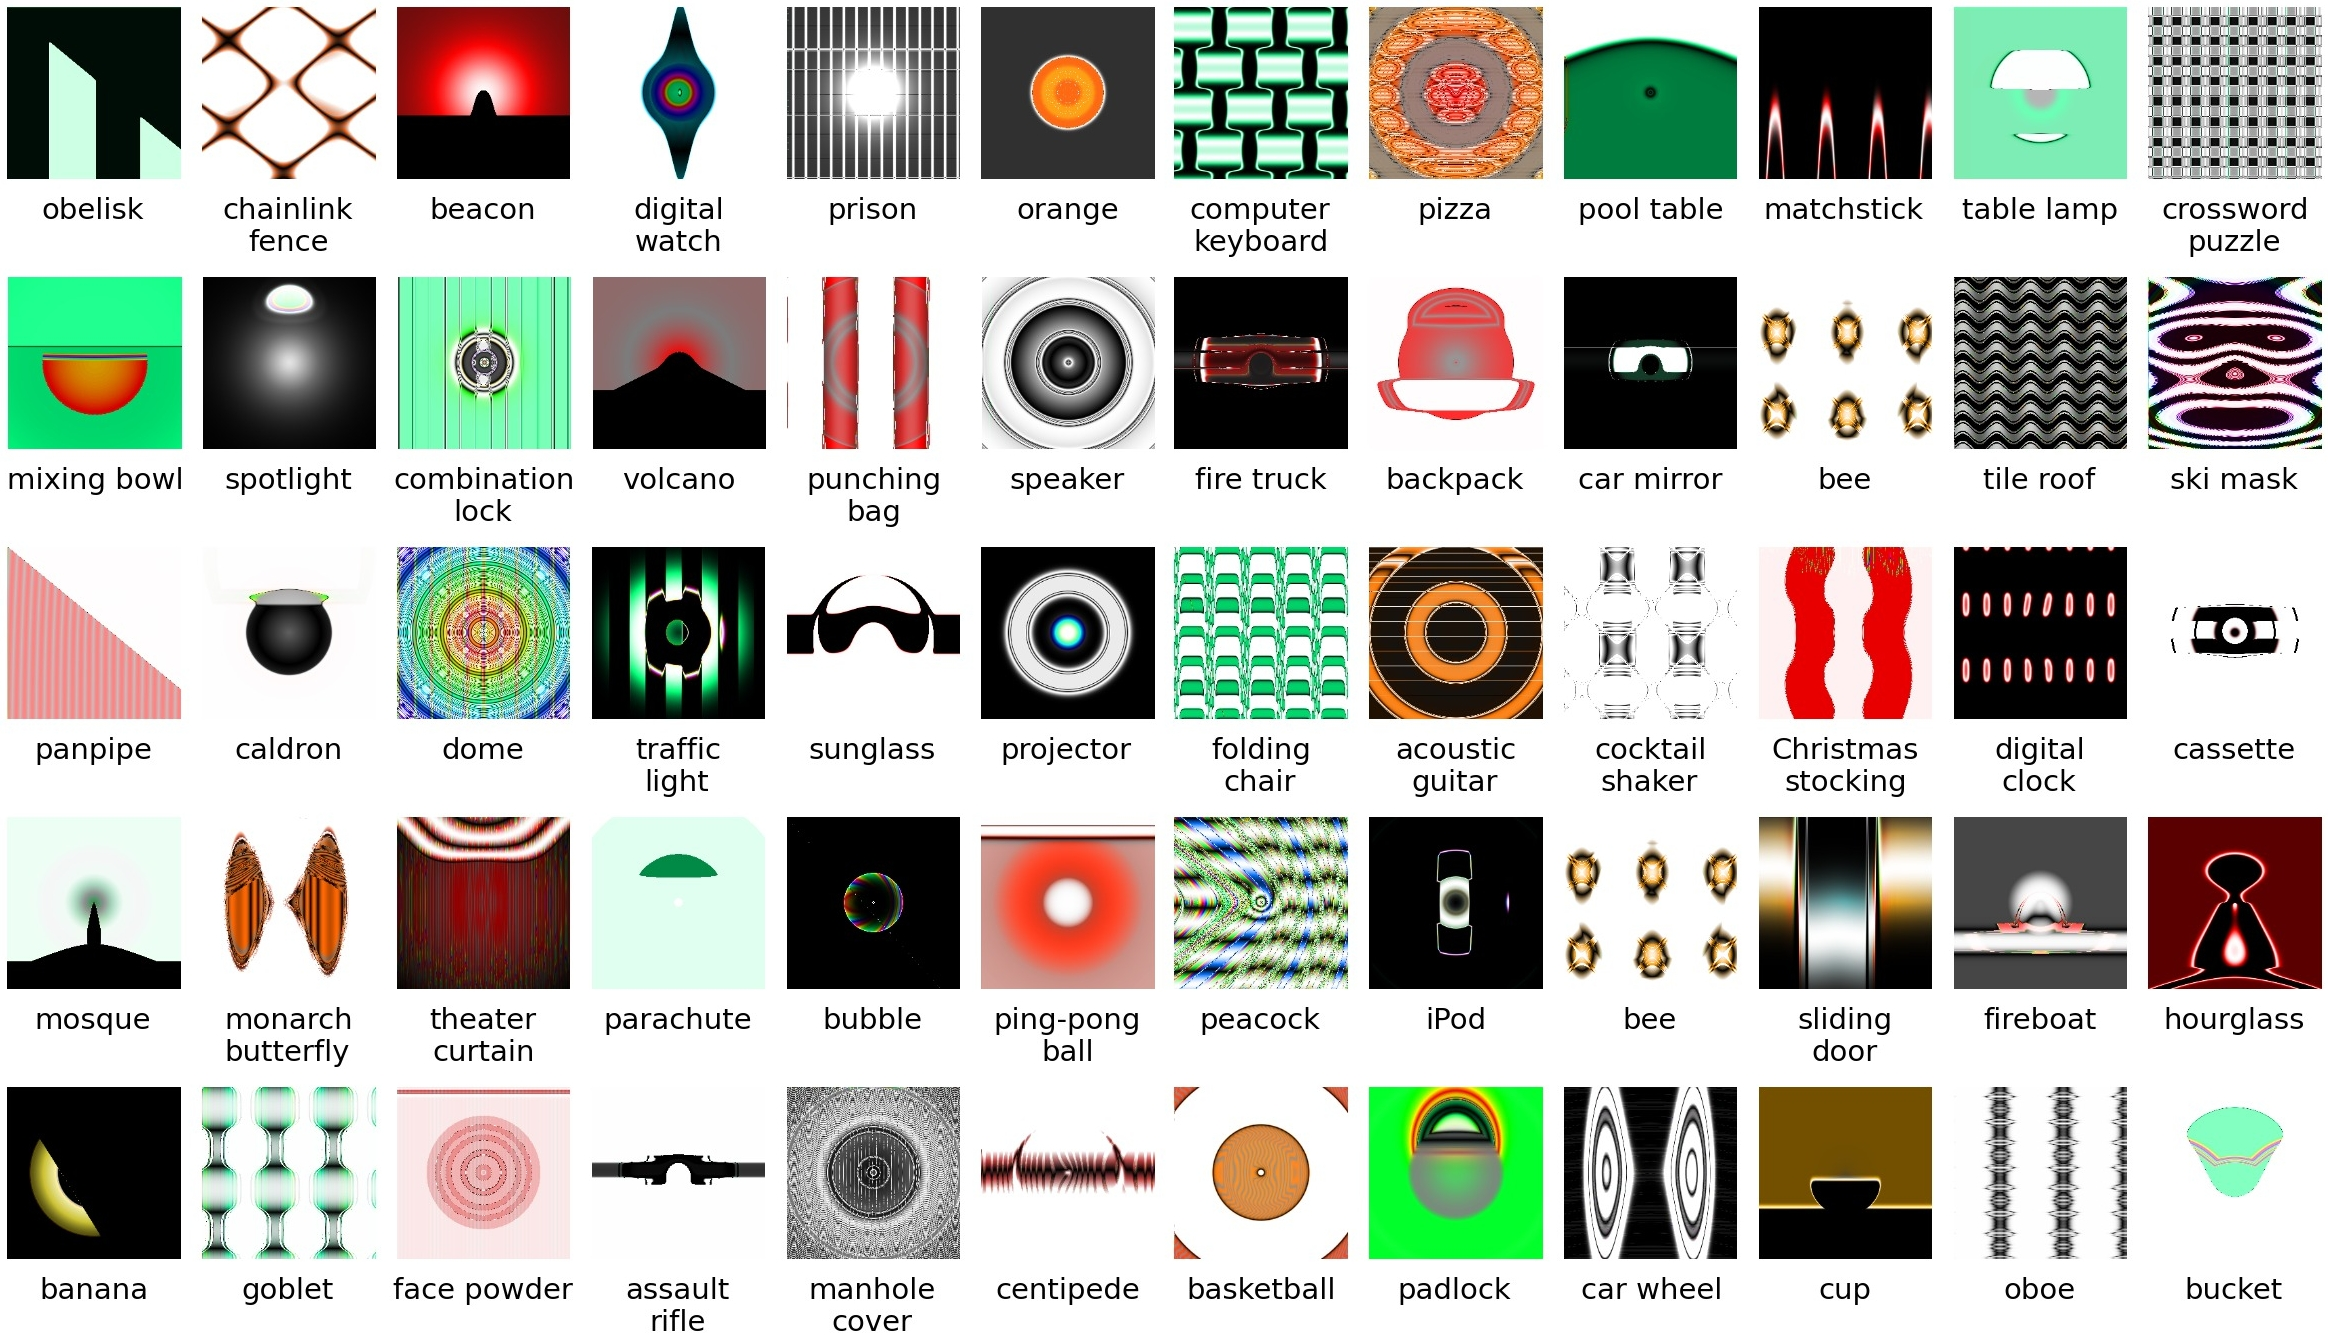
\includegraphics[width=0.9\textwidth]{img/ie_greatest_hits}
 	\captionsetup{singlelinecheck=off,justification=raggedright}
  	\caption{Selected champion individuals from a sample of environmental niches \cite[Figure 7]{Nguyen2015InnovationLearning}.}
    \label{fig:ie_results}
\end{figure}
\end{frame}

\section{Closing Thoughts}
\begin{frame}{Practical Applications}
\begin{figure}
  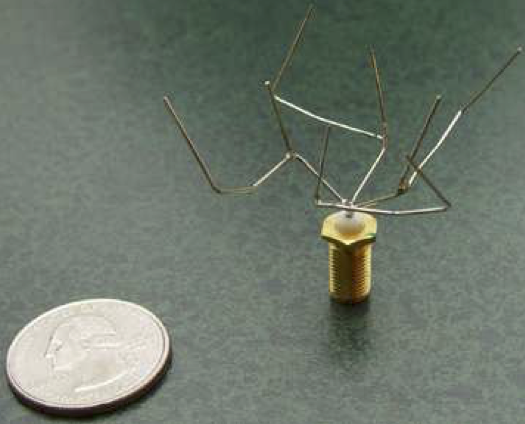
\includegraphics[width=0.7\textwidth]{img/evolved_antenna} 
  \hspace{2ex}
  \caption{A spacecraft antenna design generated using evolutionary methods \cite[Figure 2(a)]{Hornby2006AutomatedAlgorithms}.}
  \label{fig:evolved_antenna}
\end{figure}
\end{frame}

\begin{frame}{Scientific Questions}
\begin{columns}
\begin{column}{0.6\textwidth}
\begin{itemize}
\item at what level of abstraction can the power of biological evolution be harnessed in a computational model?
\item what are the fundamental mechanisms at play in evolution?
\end{itemize}
\end{column}
\begin{column}{0.4\textwidth}
\begin{center}
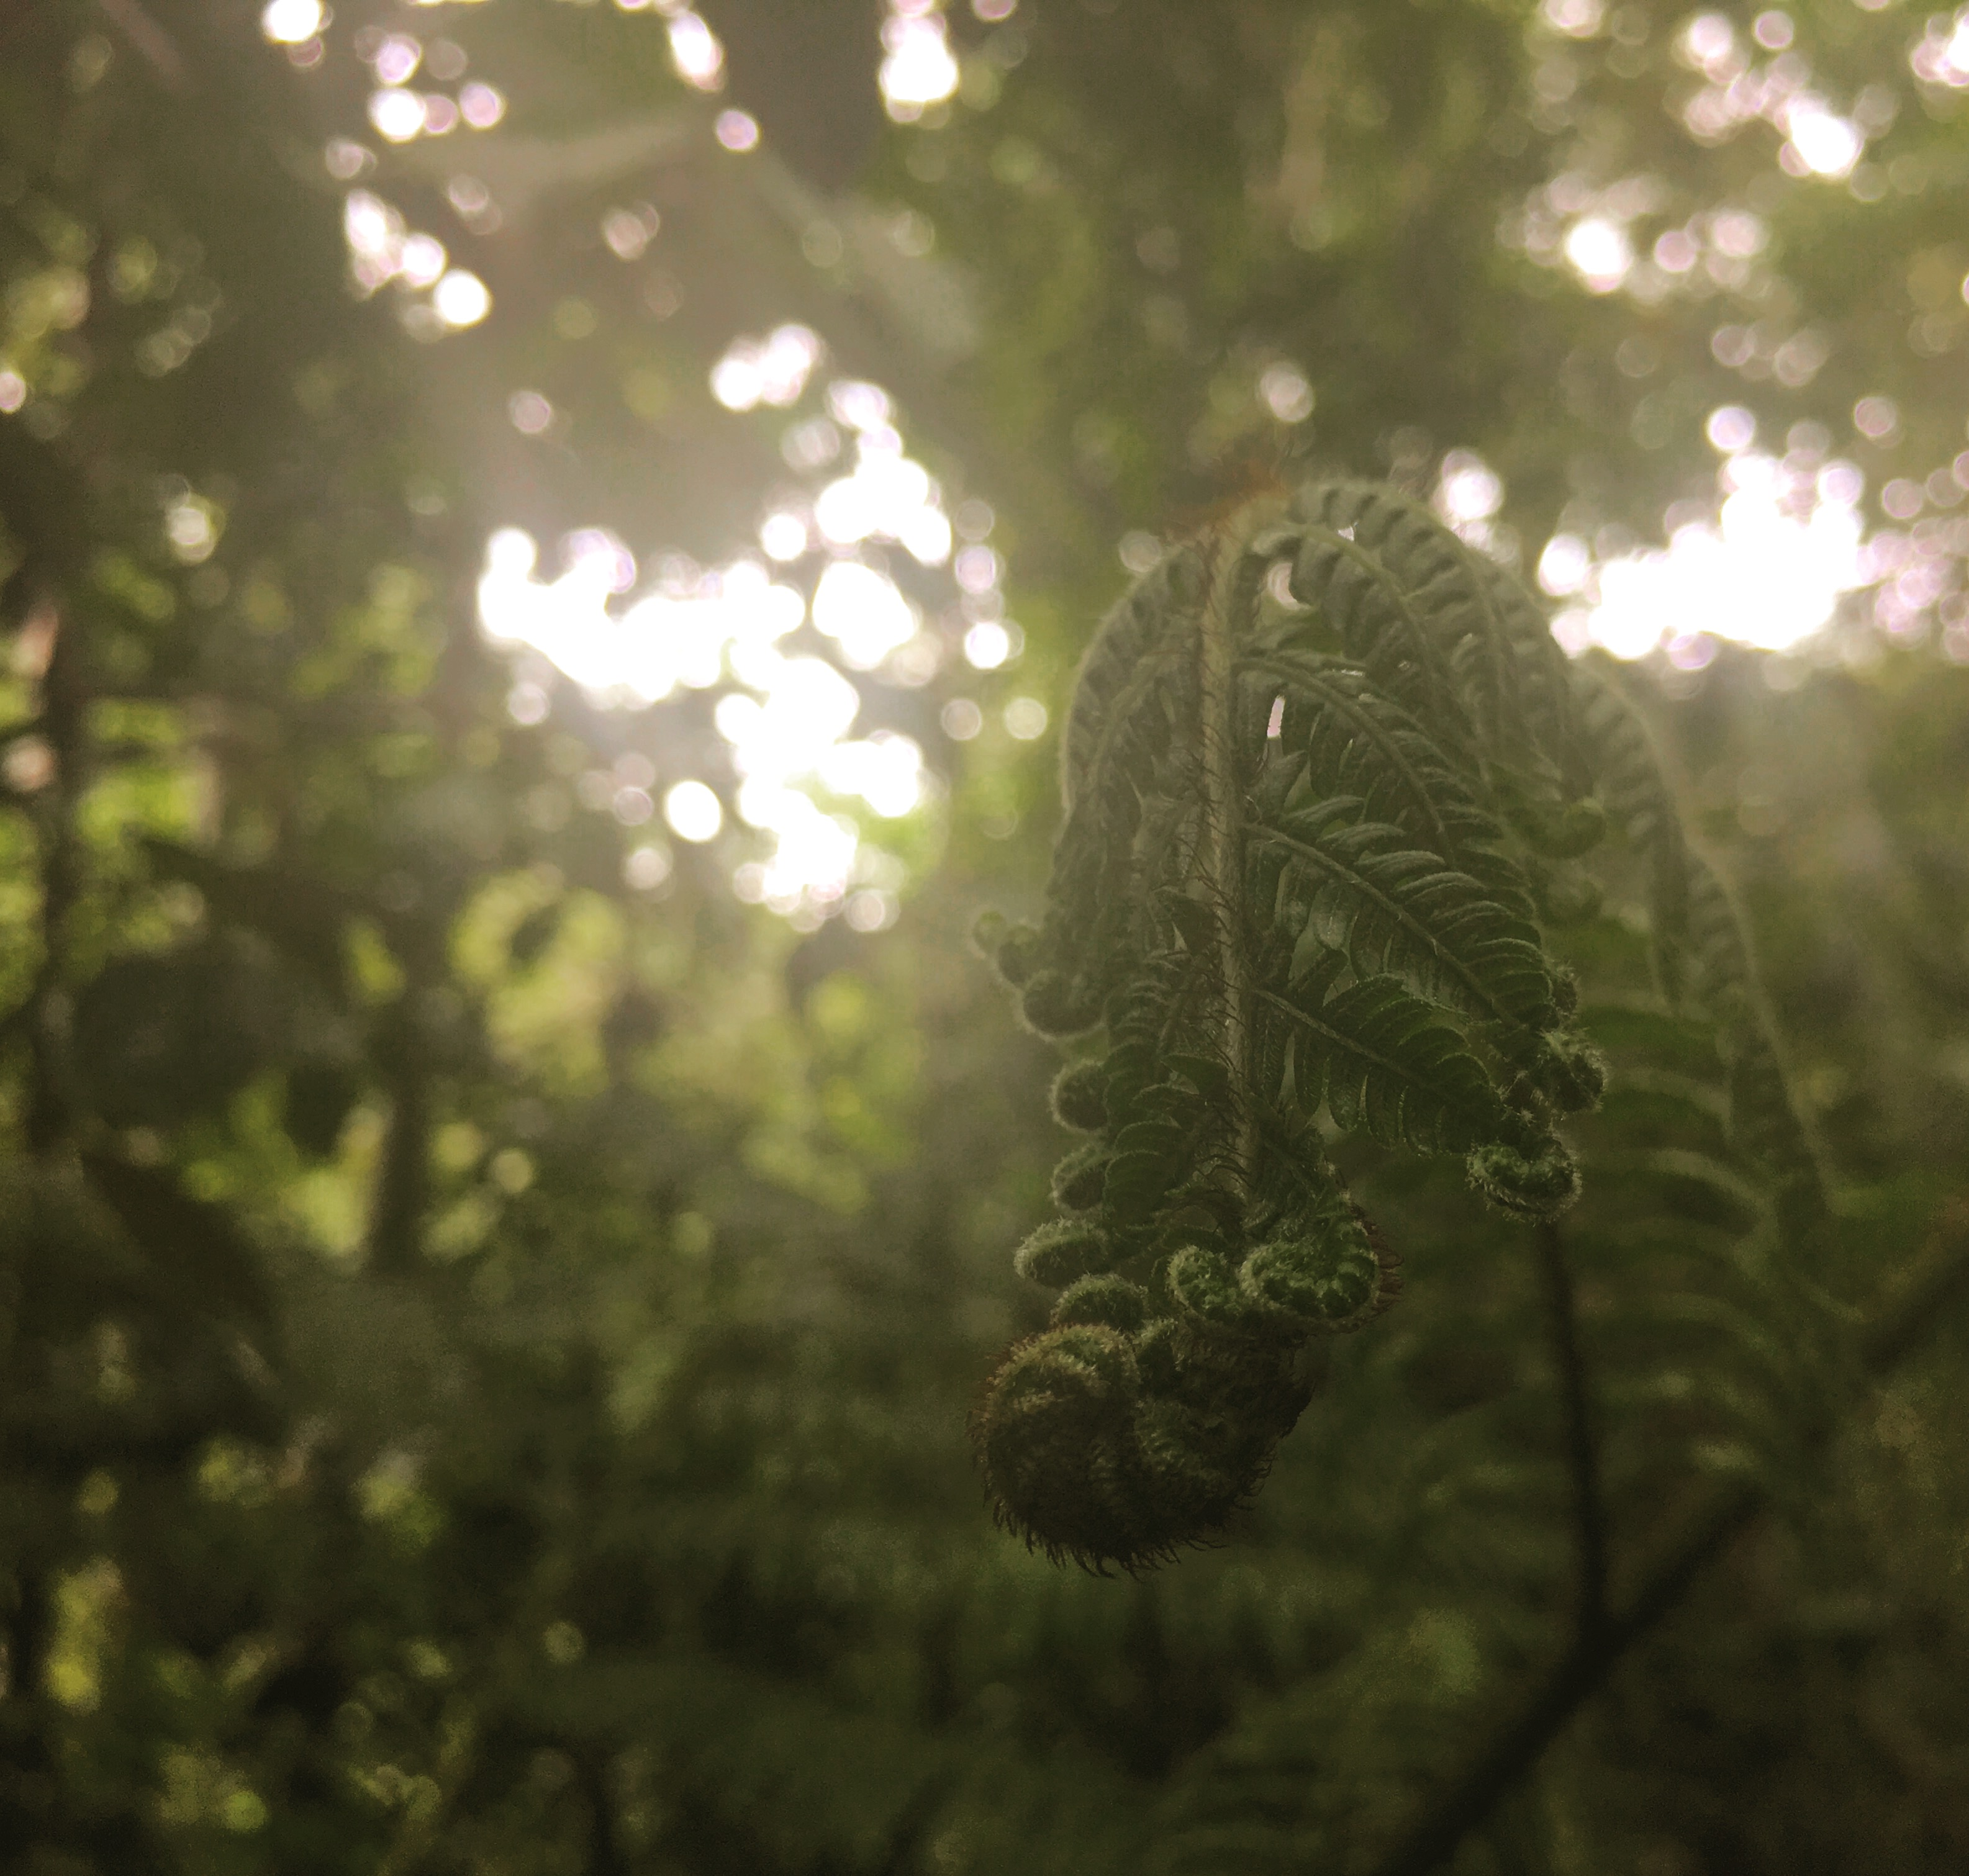
\includegraphics[width=\textwidth,trim={18cm 0 27cm 0},clip]{img/tropical_fern}
\end{center}
\end{column}
\end{columns}
\end{frame}

\begin{frame}{Scientific Questions}
\begin{columns}
\begin{column}{0.6\textwidth}
\begin{itemize}
\item evolutionary biology provides continuing inspiration for new techniques in evolutionary computing
\item evolutionary models move theory evaluation from a qualitative endeavor towards a quantitative endeavor
\end{itemize}
\end{column}
\begin{column}{0.4\textwidth}
\begin{center}
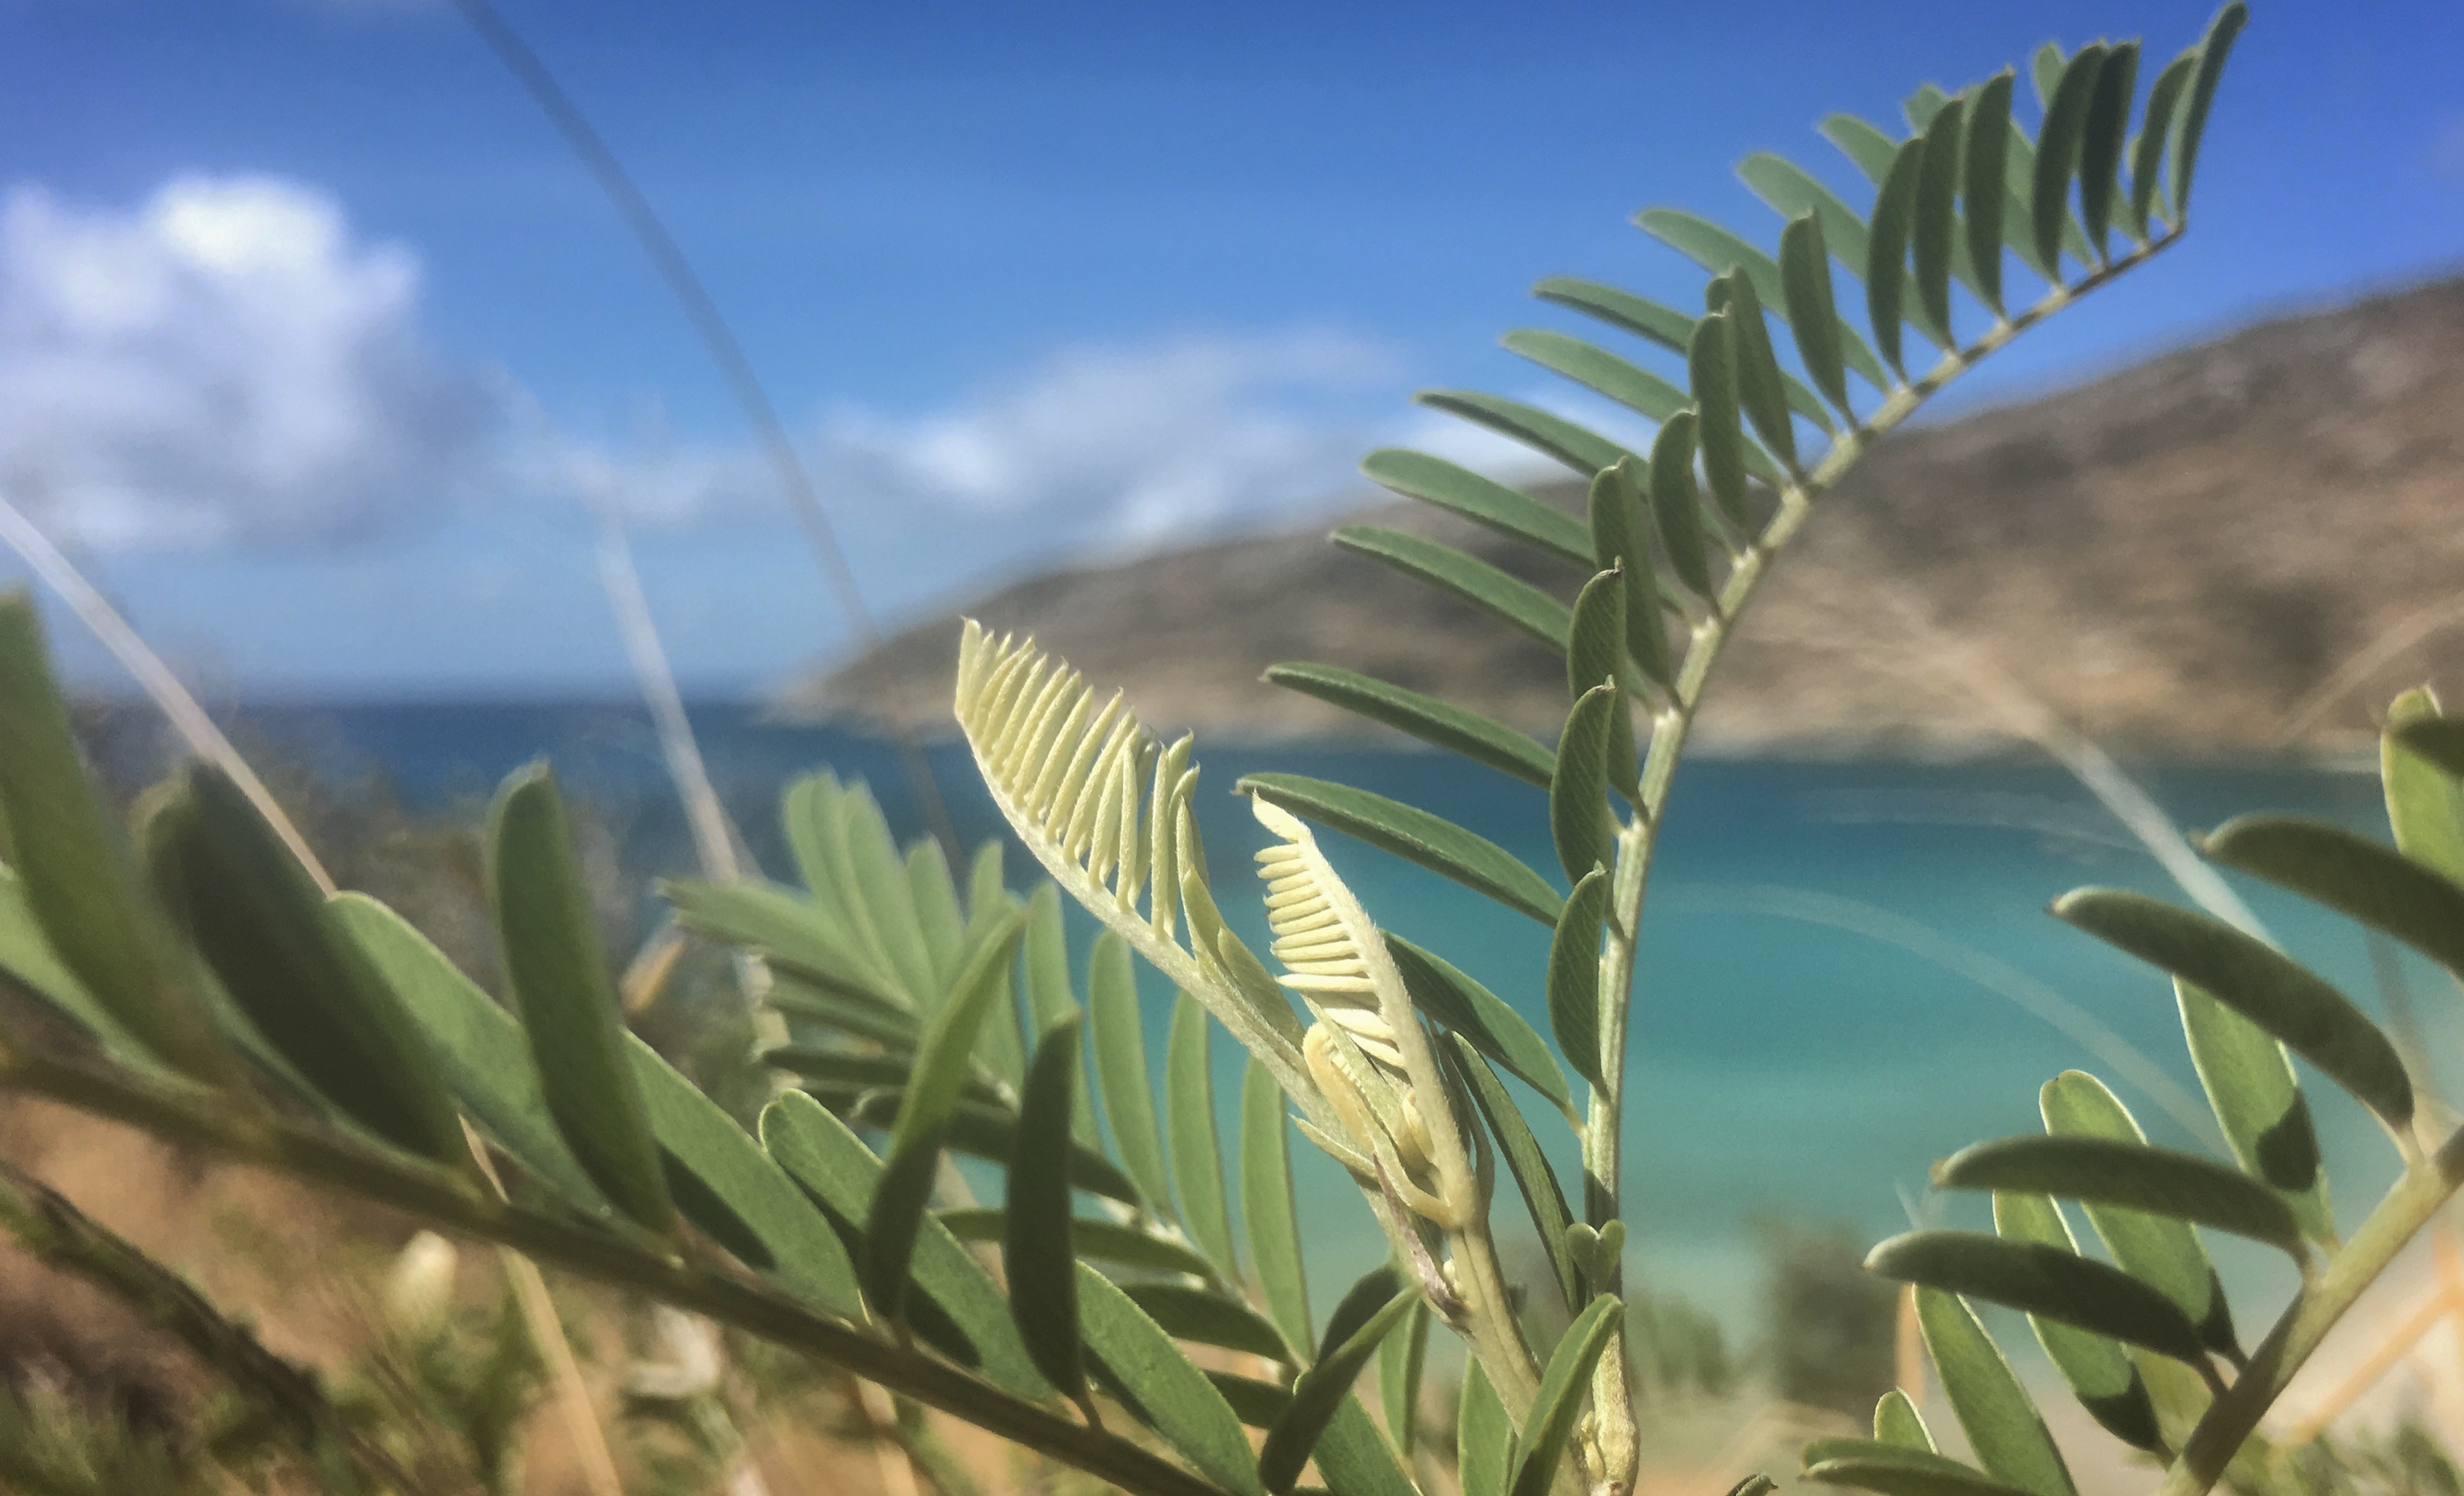
\includegraphics[width=\textwidth,trim={43cm 0 47cm 0},clip]{img/island_fern}
\end{center}
\end{column}
\end{columns}
\end{frame}

% \begin{frame}{Scientific Questions}
% \begin{displayquote}
% ``Many evolutionary biologists do not see a need to connect somatic adaptability to the generation of variation, and some see a need to keep them separate. For them, it is sufficient to say that random mutation is required and that the phenotypic variation arises haphazardly from it as random damage; the organism's current phenotype does not matter for the variation produced, and the output of variation is nearly random \cite[p 219]{Kirschner2005TheDilemma}.''
% \end{displayquote}
% \end{frame}

\appendix

\begin{frame}{Acknowledgements}
\begin{columns}
\begin{column}{0.6\textwidth}
\begin{itemize}
\item Professor Smith for serving as a thesis reader
\item Professor Erving for his support as the Honors Program Director
\item Ti for making sure it all went smoothly
\item Professor Chambers for serving as my thesis advisor
\end{itemize}
	\vspace{-1ex}
	\begin{center}{
    
\includegraphics[width= 0.4\textwidth]{img/UofPS_stacked_maroonRGB_PNG}}
    \end{center}

\end{column}
\begin{column}{0.4\textwidth}
\begin{center}
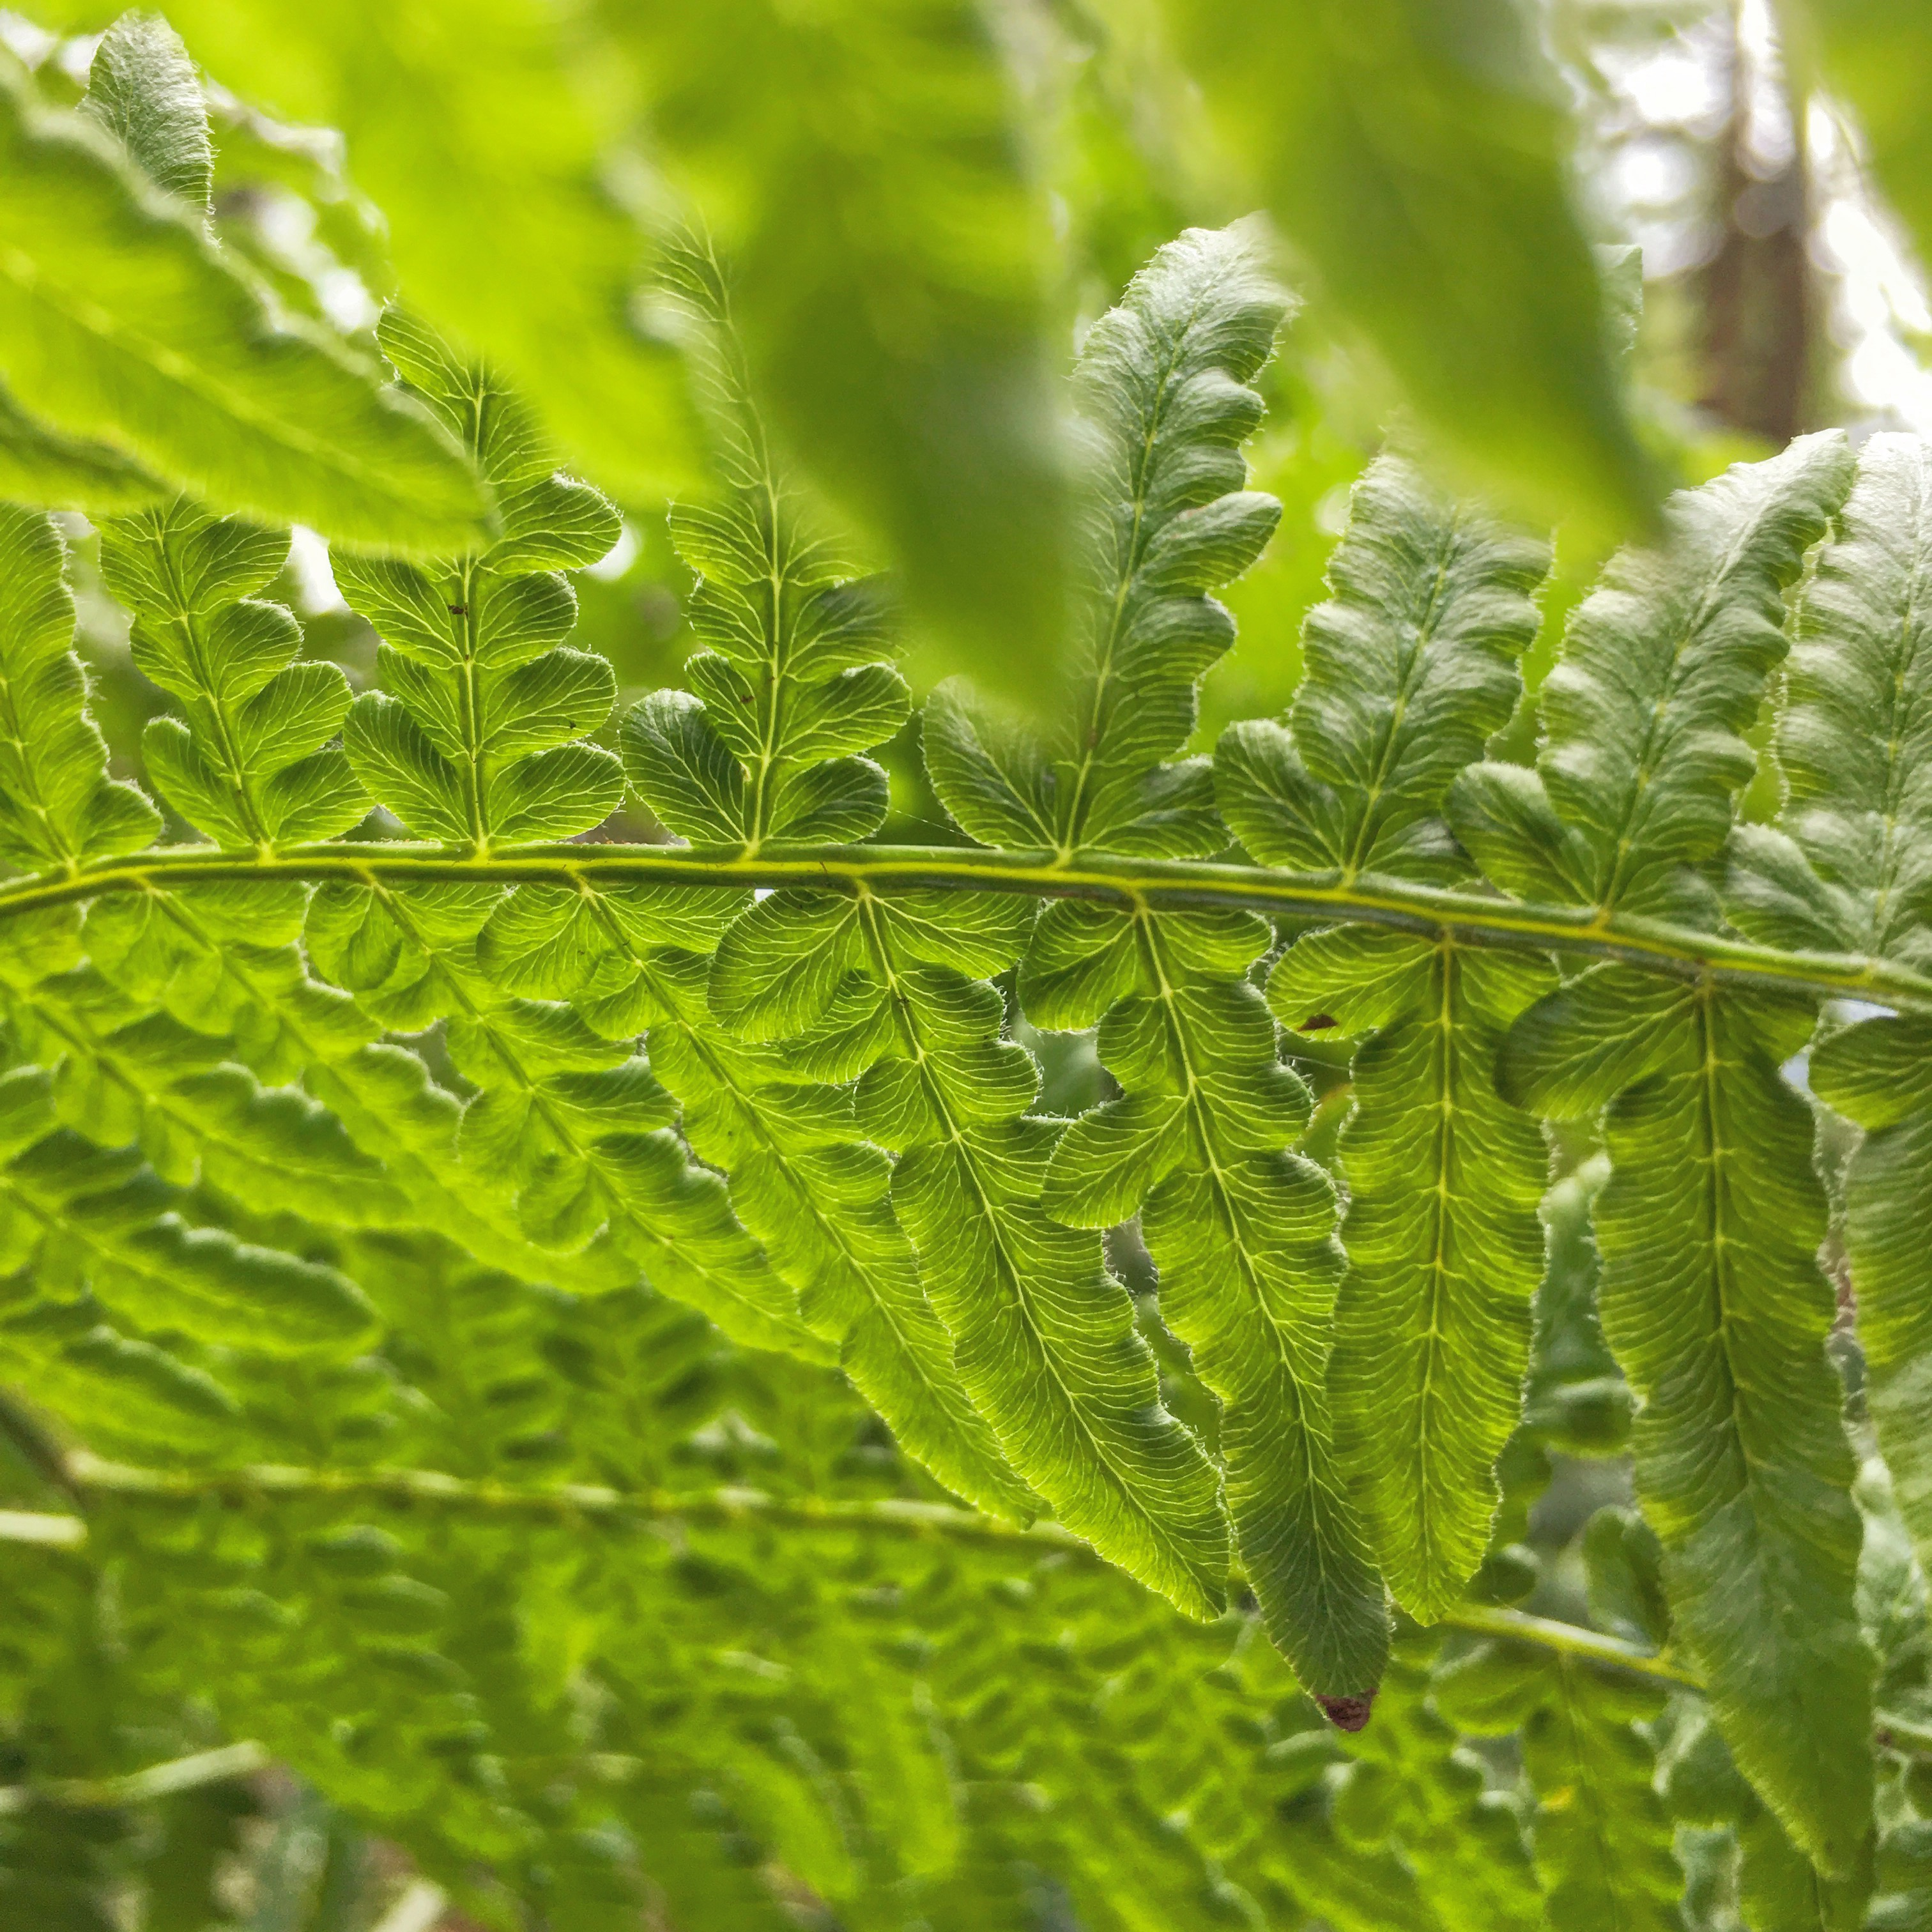
\includegraphics[width=\textwidth,trim={16cm 0 21cm 0},clip]{img/forest_fern}
\end{center}
\end{column}
\end{columns}

\end{frame}

\begin{frame}[standout]
  Questions?
\end{frame}

\begin{frame}[allowframebreaks]{References}

  \bibliography{Mendeley}
  \setbeamertemplate{bibliography item}{\insertbiblabel}
  %\nocite{*} % Insert publications even if they are not cited in the poster
  \bibliographystyle{apalike}
\end{frame}


%\begin{frame}{Evolvability as Novel Variation}
  \begin{figure}
 \centering
    \begin{subfigure}[b]{0.5\textwidth}
        \centering
    	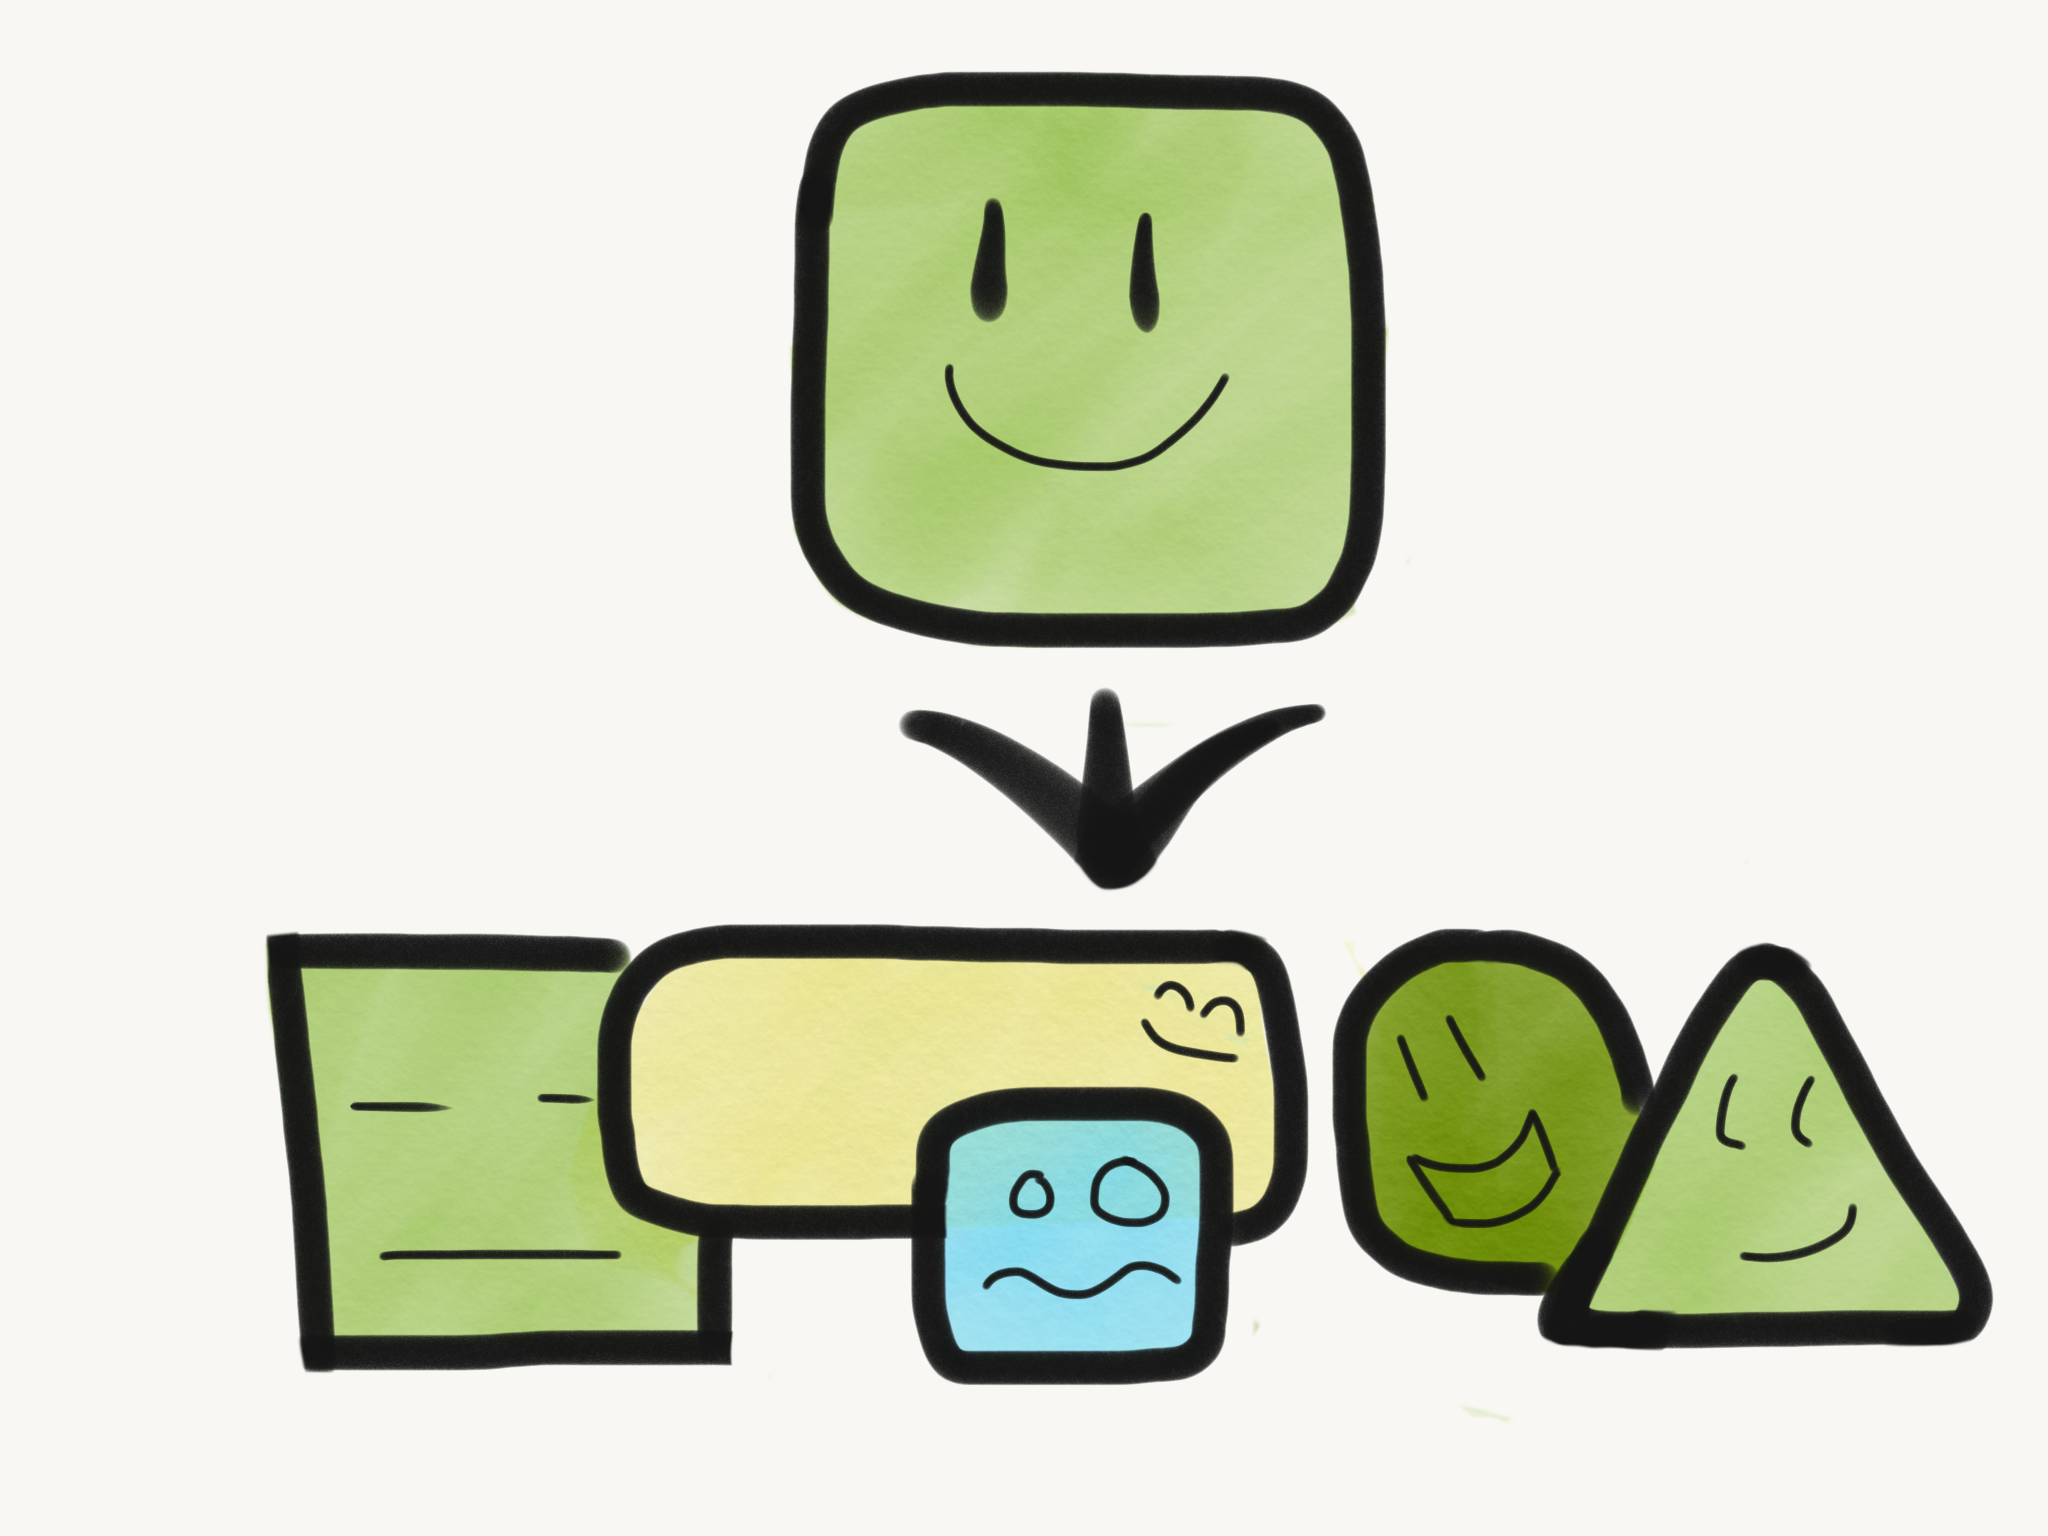
\includegraphics[width=\textwidth]{img/individual_evolvability}
        \caption{individual evolvability}
        \label{subfig:individual_evolvability}
    \end{subfigure}%
    \hfill
    \begin{subfigure}[b]{0.5\textwidth}
        \centering
        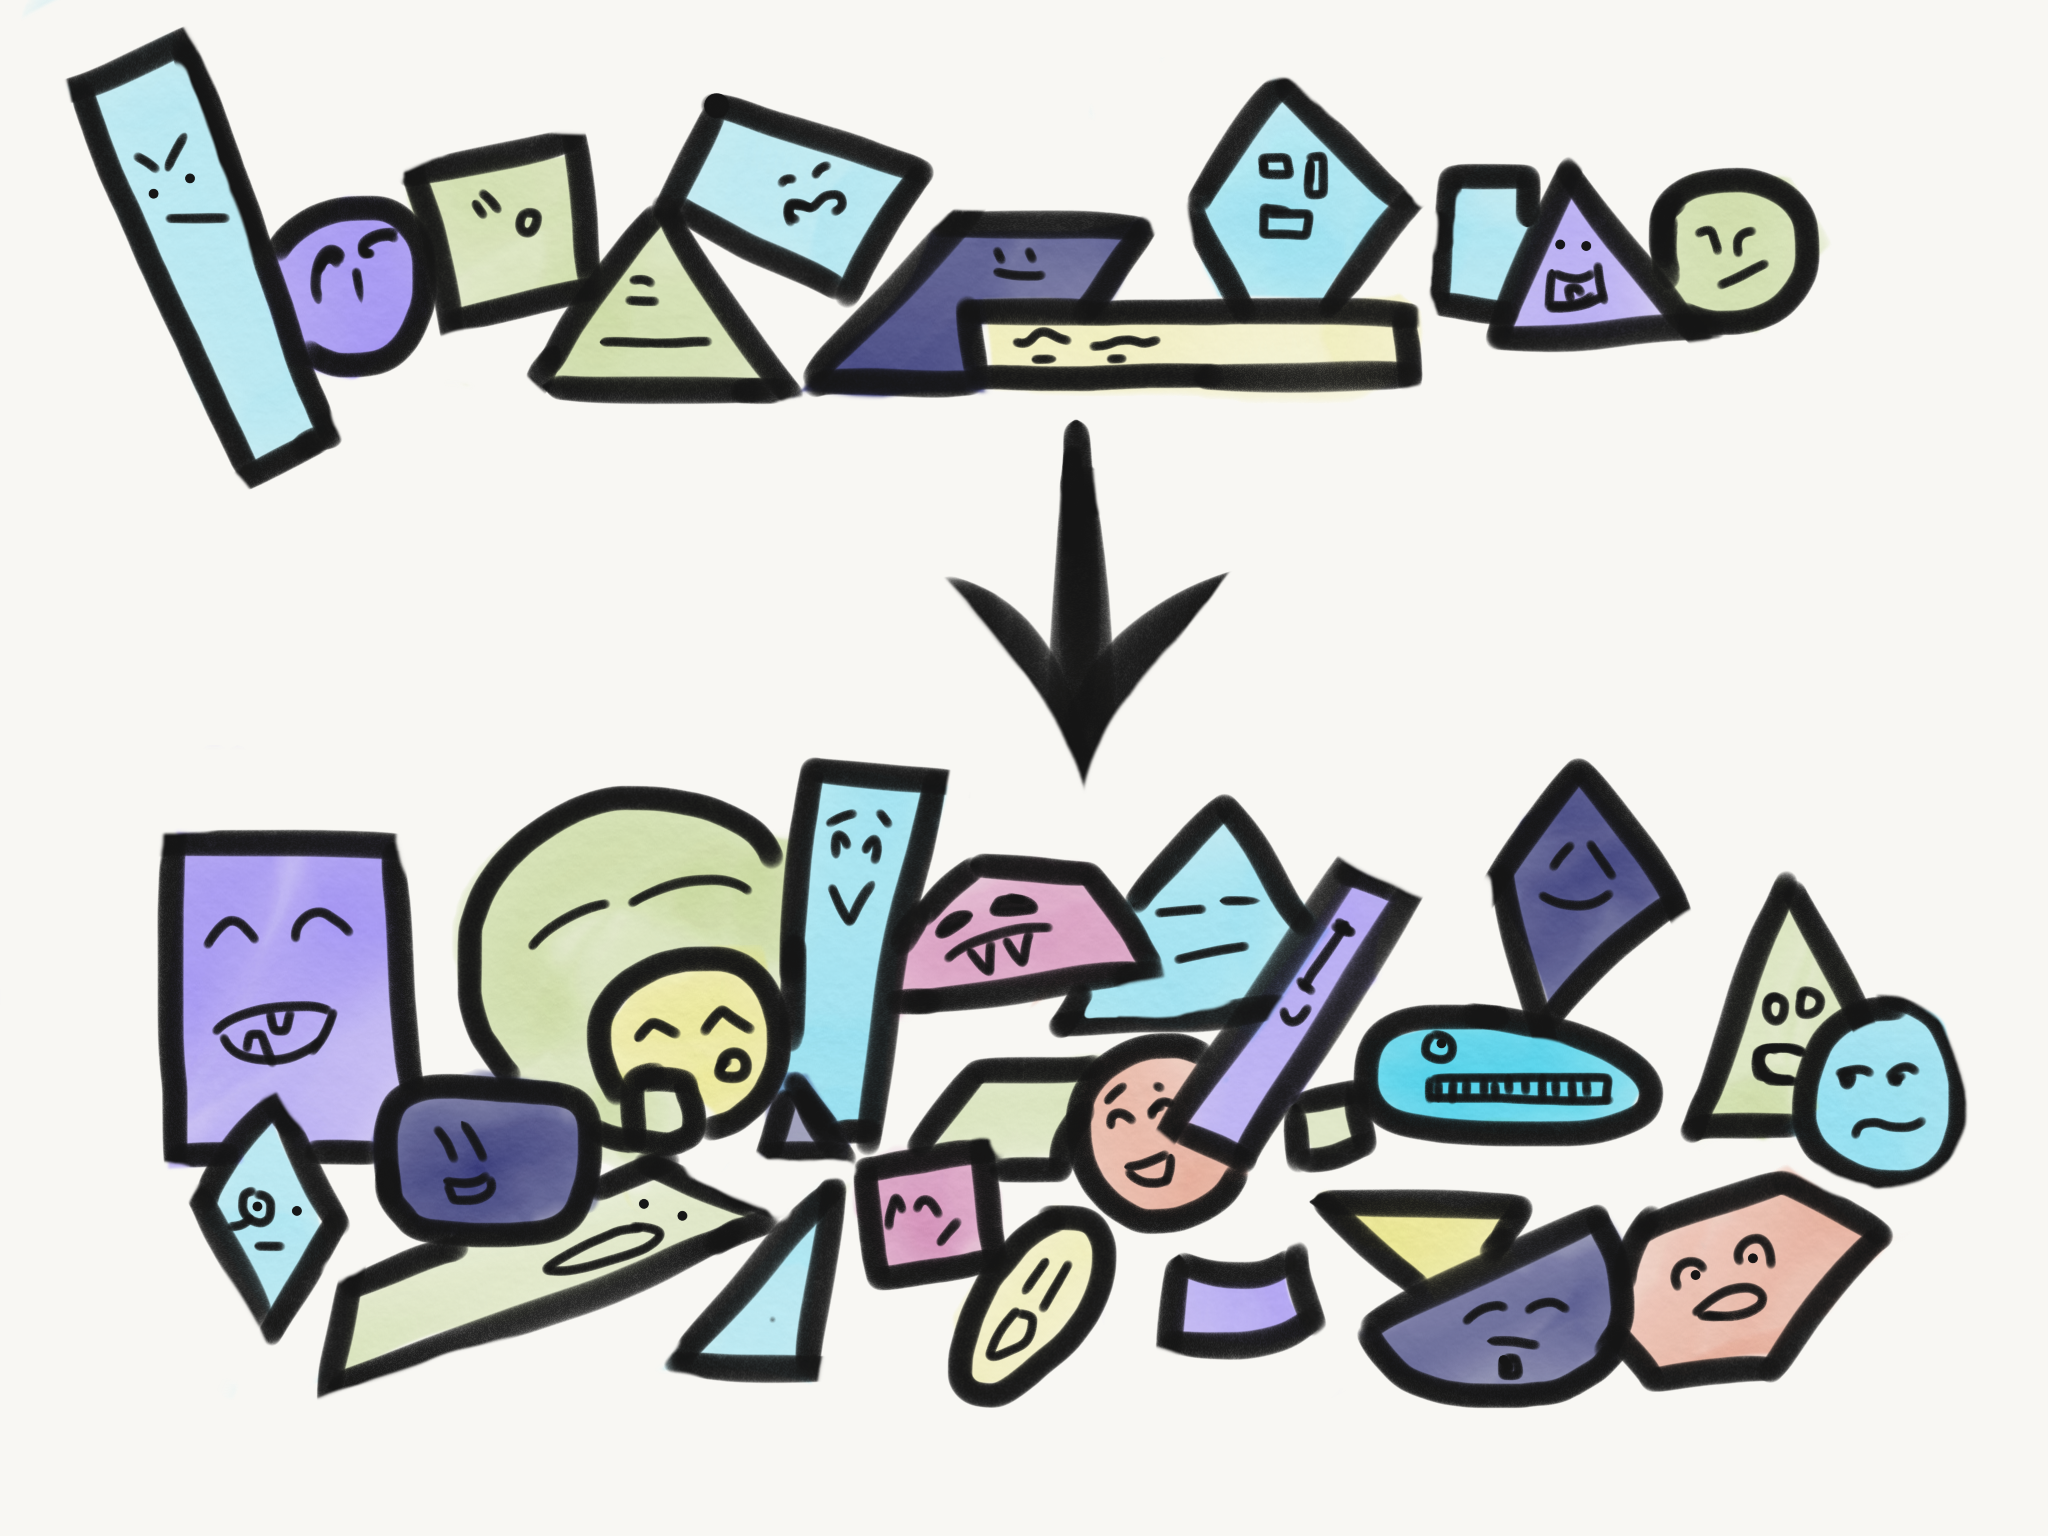
\includegraphics[width=\textwidth]{img/population_evolvability}
        \caption{population evolvability}
        \label{subfig:population_evolvability}
    \end{subfigure}
 	\captionsetup{singlelinecheck=off,justification=raggedright}
    \vspace{-4ex}
  \captionsetup{singlelinecheck=off,justification=raggedright}
  \caption{An illustration contrasting individual and population evolvability \cite{Wilder2015ReconcilingEvolvability}.}
  \label{fig:individual_vs_population_evolvability}
\end{figure}
\end{frame}

\begin{frame}{Development and the Environment}
  \begin{figure} \label{fig:elephant_developmental_perturbation}
  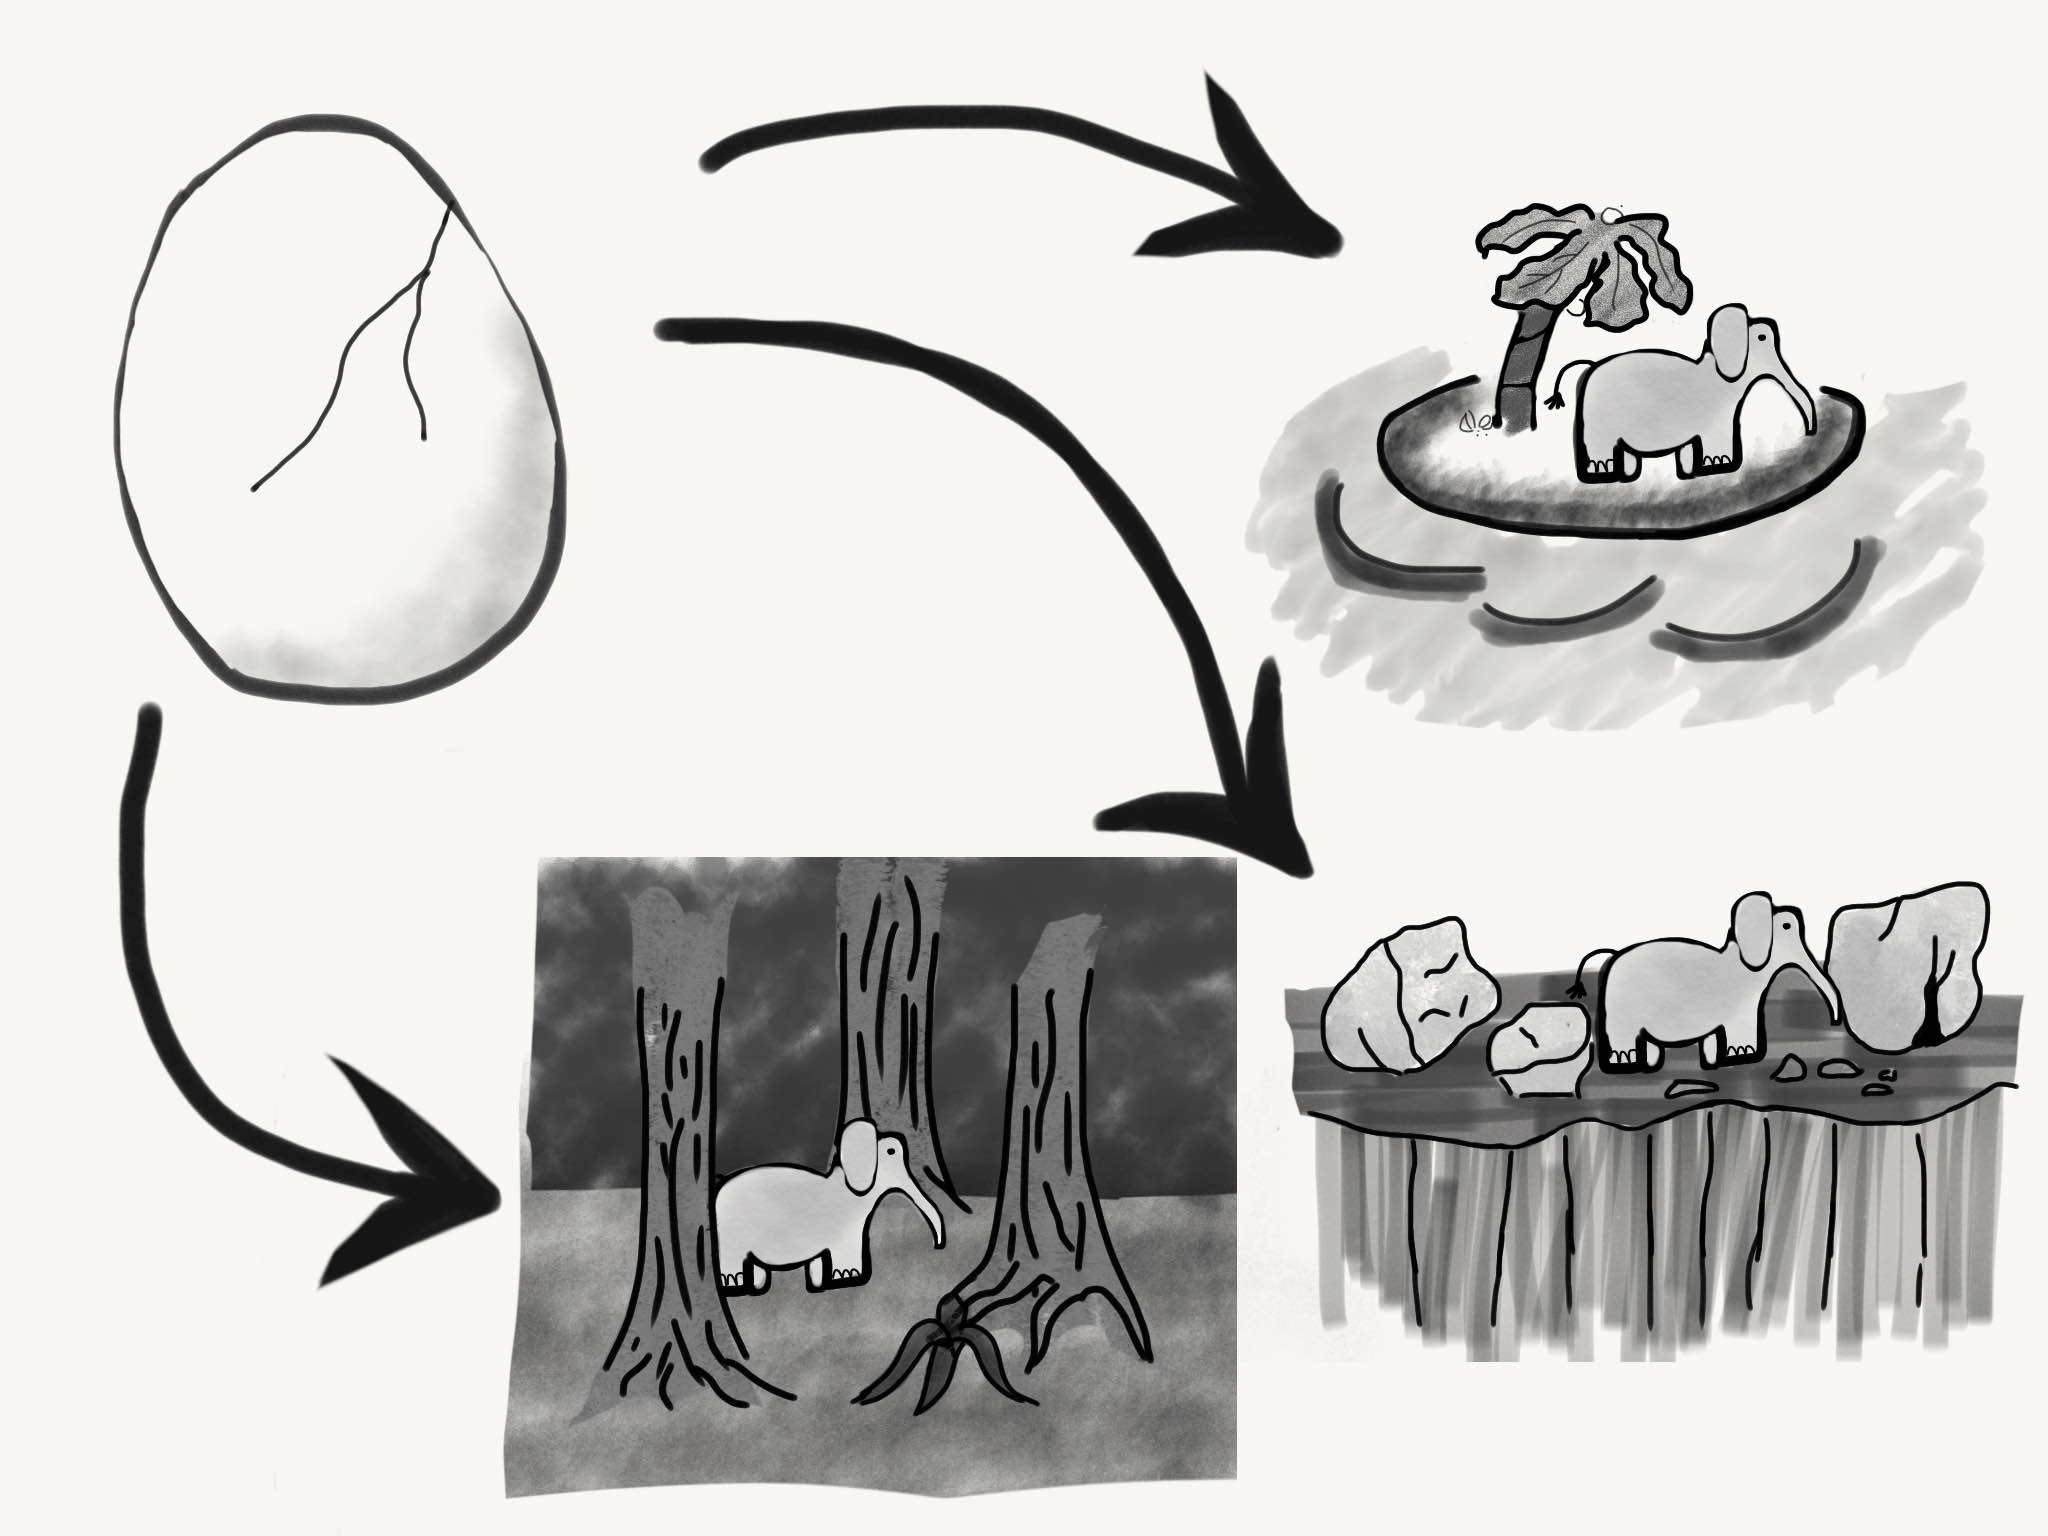
\includegraphics[width=0.8\textwidth]{img/elephant_developmental_perturbation.jpg}
  \captionsetup{singlelinecheck=off,justification=raggedright}

  \caption{An illustration of canalization against environmental perturbation}
\end{figure}
\end{frame}

\begin{frame}{Development and the Environment}
  \begin{figure} \label{figs/plant_developmental_perturbation}
  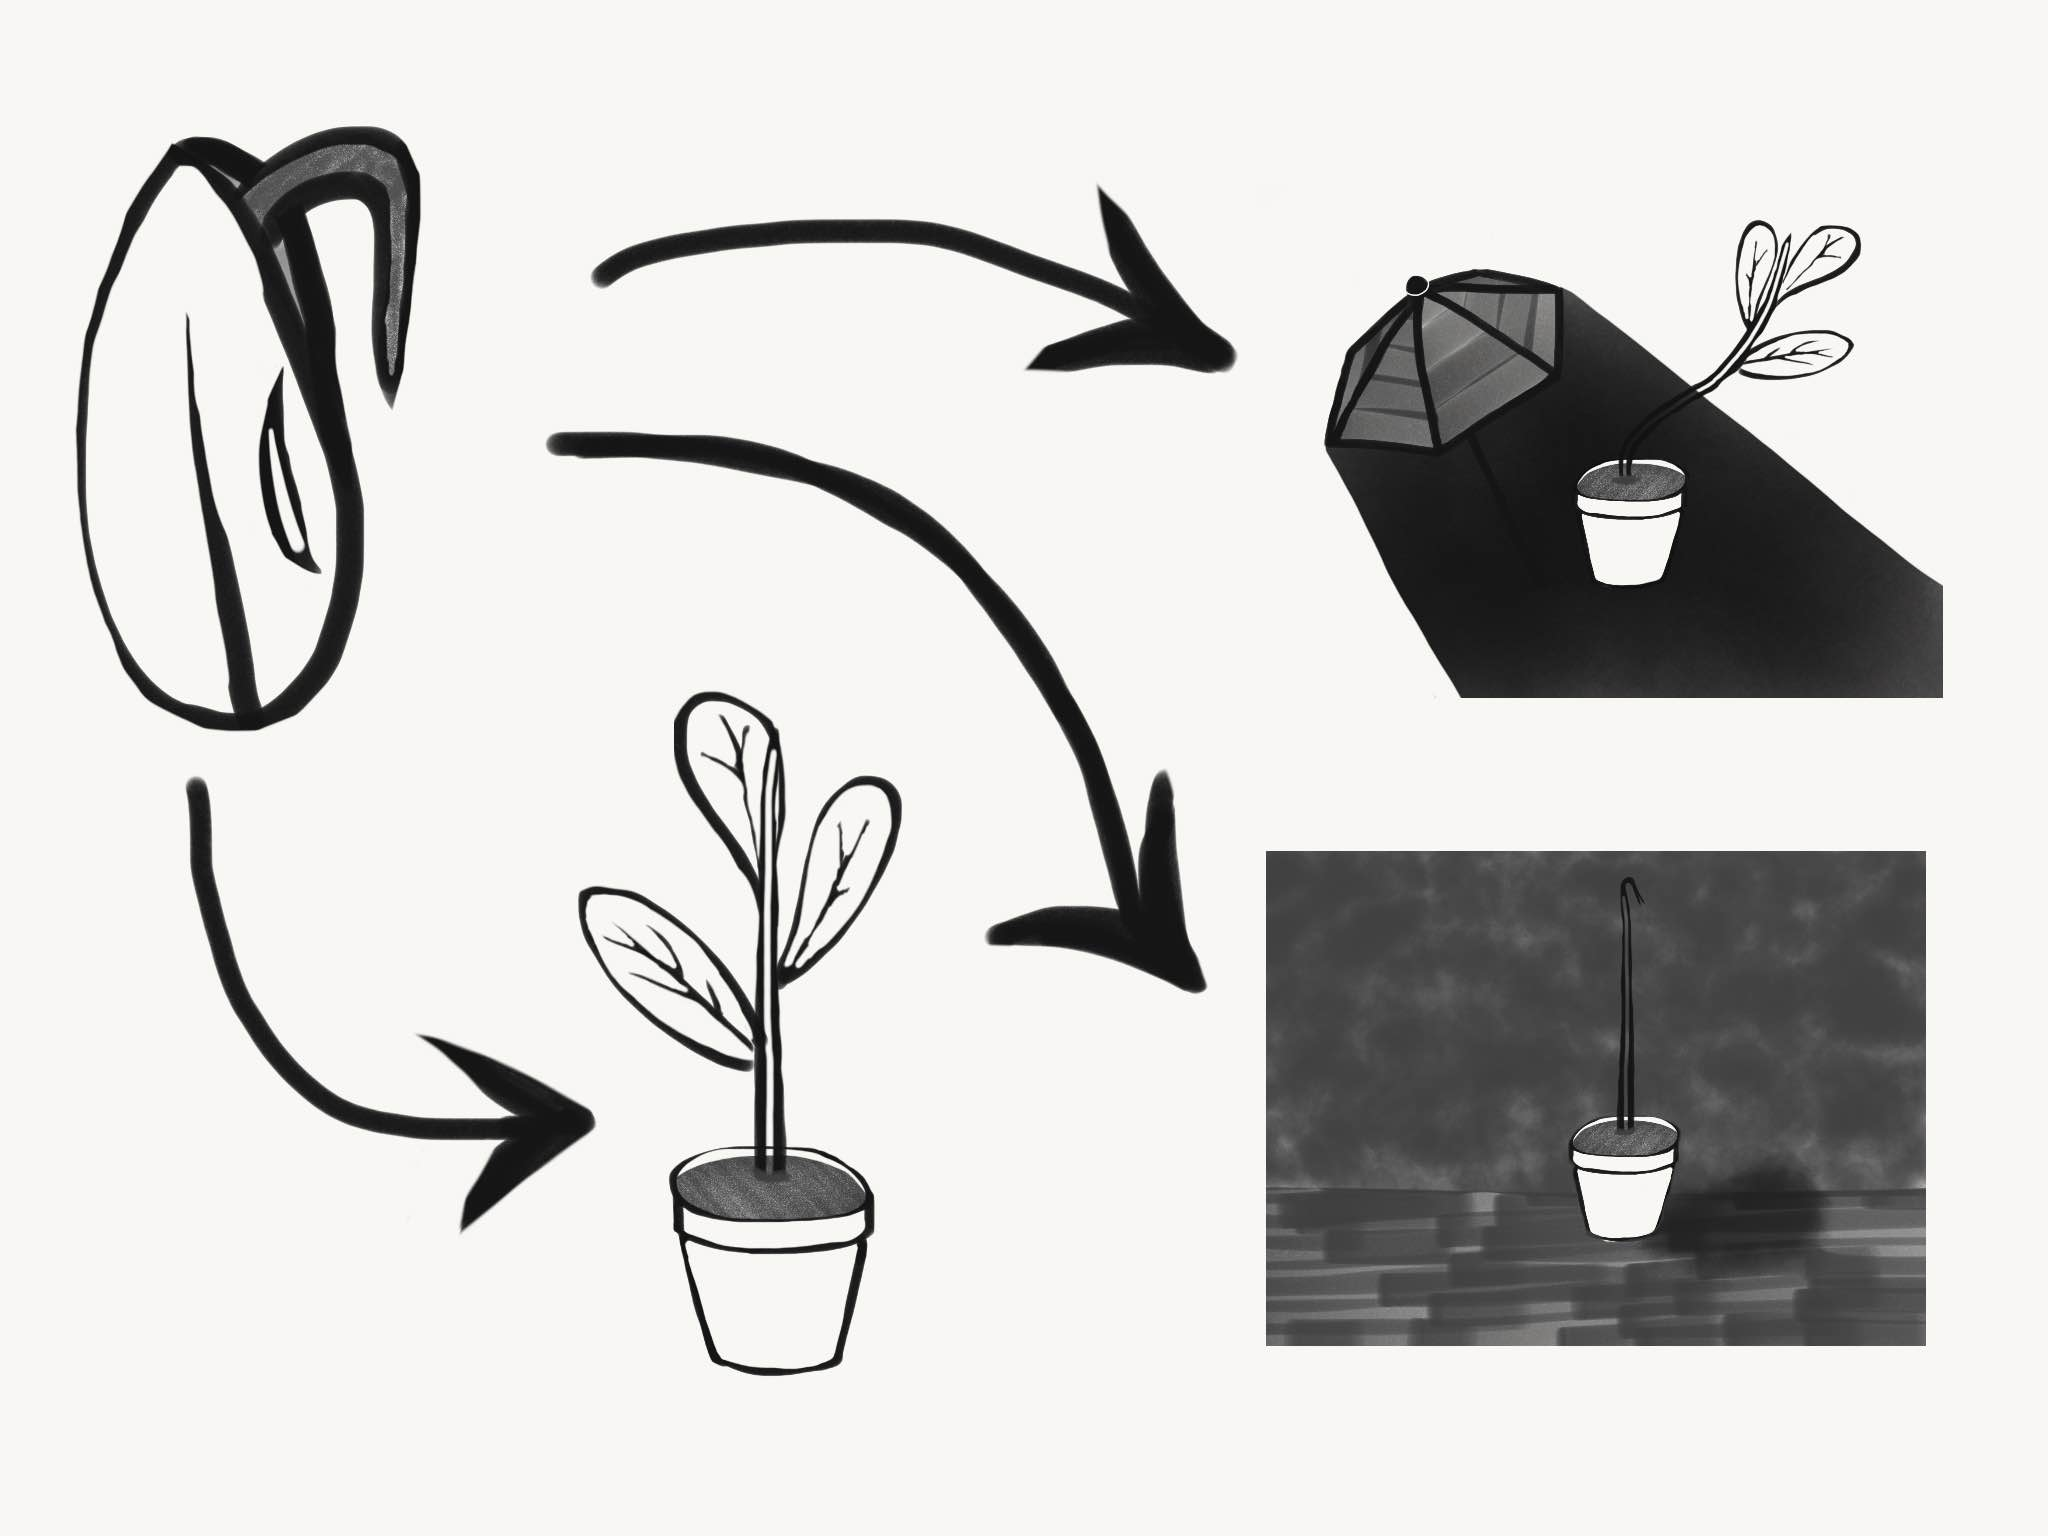
\includegraphics[width=0.8\textwidth]{img/plant_developmental_perturbation.jpg}
  \captionsetup{singlelinecheck=off,justification=raggedright}
  \caption{An illustration alternate phenotypes expressed based on environmental signals}
\end{figure}

\end{frame}



\end{document}
